\documentclass[journal]{IEEEtran}
\usepackage{amsmath,amsfonts}
\usepackage{algorithmic}
\usepackage{algorithm}
\usepackage{array}
\usepackage[caption=false,font=normalsize,labelfont=sf,textfont=sf]{subfig}
\usepackage{textcomp}
\usepackage{stfloats}
\usepackage{url}
\usepackage{verbatim}
\usepackage{graphicx}
\usepackage{cite}
\usepackage{subcaption}
\usepackage{enumitem}
\usepackage{booktabs}
\usepackage{colortbl}
\usepackage{xcolor}
\usepackage{bbding}
\usepackage{float} 
\usepackage{amssymb}

% \definecolor{cvprblue}{rgb}{0.21,0.49,0.74}
% \usepackage[pagebackref,colorlinks=true,breaklinks,citecolor=cvprblue,allcolors=cvprblue,urlcolor=cvprblue]{hyperref}

\usepackage[colorlinks,
	linkcolor=blue,
	anchorcolor=blue,
	citecolor=blue]{hyperref}

% \usepackage{ulem}
\usepackage{makecell}
\usepackage{multirow}
\definecolor{myyellow}{HTML}{FFC001}
\definecolor{myblue}{HTML}{07B2F0}
\definecolor{cvprblue}{RGB}{0,113,187}
\definecolor{lightblue}{RGB}{230, 230, 255}
\definecolor{grey}{RGB}{235,235,235}

\hyphenation{op-tical net-works semi-conduc-tor IEEE-Xplore}
% updated with editorial comments 8/9/2021

\begin{document}

\title{
% Unified Temporal Autoregressive Modeling with Scale-Wise Flow Matching for Action-Conditioned World Models 
Unified Temporal Autoregression and Scale-Wise Flow Matching for Embodied World Models
% Continuous Scale-Wise Flow Matching for Action-Conditioned Embodied World Models
% Bridging Causal Reasoning and Continuous Synthesis: A Predict-then-Refine World Model for Embodied Control
% A Unified Framework for Action-conditioned World Models via Autoregressive Modeling with Scale-Wise Flow Matching
% Unified Visual Autoregressive Modeling with  for Scalable Interactive World Models
}


\author{Sen Wang, %~\IEEEmembership{Student Member, IEEE,}
        Sanping Zhou,~\IEEEmembership{Member, IEEE,} 
        Huaiyi Dong, %~\IEEEmembership{Student Member, IEEE,} 
        Kun Xia,~\IEEEmembership{Member, IEEE,} \\
        Gang Hua,~\IEEEmembership{Fellow, IEEE,}
        and Le Wang,~\IEEEmembership{Senior Member, IEEE}% <-this % stops a space
        
\thanks{Manuscript received xxx; revised xxx; accepted xxx. Date of publication xxx; date of current version xxx. 
This work was supported in part by the National Key Research and Development Project under Grant 2024YFB4708100, the Fundamental and Interdisciplinary Disciplines Breakthrough Plan of the Ministry of Education of China under Grant JYB2025XDXM504, National Natural Science Foundation of China under Grants 62572384, U24A20325, 62125305, 62503384, and Key Research and Development Plan of Shaanxi Province under Grant 2024PT-ZCK-80. (\textit{Corresponding author: Sanping Zhou.})

Sen Wang, Sanping Zhou, Huaiyi Dong and Le Wang are with the State Key Laboratory of Human-Machine Hybrid Augmented Intelligence, Institute of Artificial Intelligence and Robotics, Xi'an Jiaotong University, Xi’an 710049, China (e-mail: sen.wang@stu.xjtu.edu.cn; spzhou@mail.xjtu.edu.cn; Donghuaiyi@stu.xjtu.edu.cn; lewang@mail.xjtu.edu.cn;). 
Kun Xia is also with the School of Computer Science and Technology, Xi’an Jiaotong University, Xi’an 710049, China (e-mail: kunxia@mail.xjtu.edu.cn). 
Gang Hua is with Amazon Alexa AI, Bellevue, WA 98004 USA (e-mail: ganghua@gmail.com).
}% <-this % stops a space
% \thanks{The source code is available at \href{https://github.com/SanMumumu/FlowRAM/tree/Flow2Act}{https://github.com/SanMumumu/Flow2Act}}
}

% The paper headers
\markboth{Journal of \LaTeX\ Class Files,~Vol.~XXX, No.~XXX, June~2026}%
{Shell \MakeLowercase{\textit{et al.}}: A Sample Article Using IEEEtran.cls for IEEE Journals}

\IEEEpubid{0000--0000/00\$00.00~\copyright~2026 IEEE}
% Remember, if you use this you must call \IEEEpubidadjcol in the second
% column for its text to clear the IEEEpubid mark.

\maketitle



\begin{abstract}

Action-conditioned world models are fundamental for embodied agents to simulate future environments and execute long-horizon planning. Yet, current methodologies struggle with a persistent dichotomy: discrete autoregressive models offer robust causal reasoning but suffer from quantization artifacts and resolution bottlenecks, while continuous generative models yield high perceptual fidelity but lack the structured temporal consistency necessary for reliable planning. 
To bridge this divide, we propose SAMPO++, a unified framework that seamlessly integrates temporal autoregressive modeling with scale-wise flow matching within a fully continuous latent space. 
At its core, SAMPO++ introduces a novel ``Predict-then-Refine" paradigm: a temporal autoregressive transformer first establishes coarse-grained structural priors for future states, which a scale-wise flow matching generator subsequently refines to synthesize high-fidelity details from noise. 
To achieve precise controllability, we design an Action-adaptive Dynamics Modulation (ADM) mechanism that injects action signals into feature statistics via scale-aware affine transformations. 
Moreover, we mitigate long-term structural degradation by incorporating Scale-Aware spacetime Rotary Position Embeddings (SA-RoPE) alongside a flow trajectory rectification strategy, thereby enforcing rigorous spatiotemporal coherence.
Extensive empirical evaluations demonstrate that SAMPO++ significantly surpasses state-of-the-art discrete and continuous baselines in video prediction quality, dynamic consistency, and control responsiveness, setting a new benchmark for high-fidelity continuous world modeling.
% Videos, code, and more details are available at \href{https://sanmumumu.github.io/Flow2Act/}{project page}.



\end{abstract}

\begin{IEEEkeywords}
World Model, Autoregressive Modeling, Continuous Representation Learning.
\end{IEEEkeywords}
\section{Introduction}
\label{sec1:Intro}

\IEEEPARstart{T}{he} development of autonomous agents capable of reasoning, planning, and executing complex tasks within dynamic environments remains a paramount objective in artificial intelligence. Central to this pursuit is the paradigm of World Models~\cite{ha2018world, hafner2019dream}, internal predictive engines that empower agents to forecast the spatiotemporal consequences of their actions before physical interaction. Contemporary theoretical frameworks~\cite{lecun2022path} posit that a robust world model serves as the cognitive substrate for intelligent systems. It facilitates learning from sparse rewards and enables planning over extended horizons by synthesizing potential future trajectories~\cite{hafner2020dreamerv2, hafner2023dreamerv3}. Consequently, constructing world models that simultaneously achieve high perceptual fidelity, strict spatiotemporal consistency, and precise action-controllability has emerged as a critical imperative across the computer vision and robotics communities~\cite{bruce2024genie, wu2024ivideogpt, wang2025sampo}.

Despite substantial advancements, visual world modeling remains bifurcated into two dominant paradigms, each with distinct theoretical merits and inherent limitations. The first, \textbf{Discrete Autoregressive Modeling}~\cite{van2017neural, esser2021taming}, formulates video generation as a sequence modeling task over quantized latent tokens. By discretizing continuous visual signals into finite codebook indices via mechanisms like VQ-VAE~\cite{van2017neural} or VQGAN~\cite{esser2021taming}, these frameworks leverage the powerful causal reasoning capabilities of transformers~\cite{vaswani2017attention, brown2020language} to predict future states sequentially~\cite{yan2021videogpt, rakhimov2020latent}. While highly effective at capturing macro-level semantic structures and maintaining causal consistency, this approach is fundamentally hindered by a quantization bottleneck. The discrete nature of finite codebooks imposes an intrinsic ceiling on visual fidelity, which frequently manifests as temporal flickering, the degradation of fine-grained textures, and an inability to model continuous physical dynamics (\textit{e.g.}, fluid turbulence or subtle illumination gradients)~\cite{yu2023magvit, yu2023language}. Furthermore, scaling the codebook capacity to mitigate these artifacts incurs prohibitive computational overhead.

%%%%%%%%%%%%%%%%%%
\IEEEpubidadjcol 
%%%%%%%%%%%%%%%%%%

Conversely, the second paradigm comprises \textbf{Continuous Generative Models}, notably Diffusion Probabilistic Models (DPMs)~\cite{ho2020denoising, rombach2022high} and emerging Flow Matching architectures~\cite{lipman2023flow, liuflow}. Operating directly within continuous latent manifolds, these methodologies successfully circumvent quantization errors, thereby achieving state-of-the-art perceptual quality~\cite{peebles2023scalable, liu2024sora, blattmann2023stable}. Nevertheless, they often lack the explicit, structured reasoning capabilities demanded by long-horizon planning. Standard continuous generative architectures frequently fail to preserve object permanence and temporal coherence during extended rollouts, primarily because they lack the strong causal inductive biases inherent to autoregressive systems. Furthermore, embedding precise action-conditional control into these continuous spaces remains a non-trivial challenge; naive concatenation of action vectors typically proves insufficient for effectively modulating the fine-grained kinematic dynamics of the generated scenes~\cite{zhang2023adding, mou2024t2i}.

\begin{figure*}
    \centering
    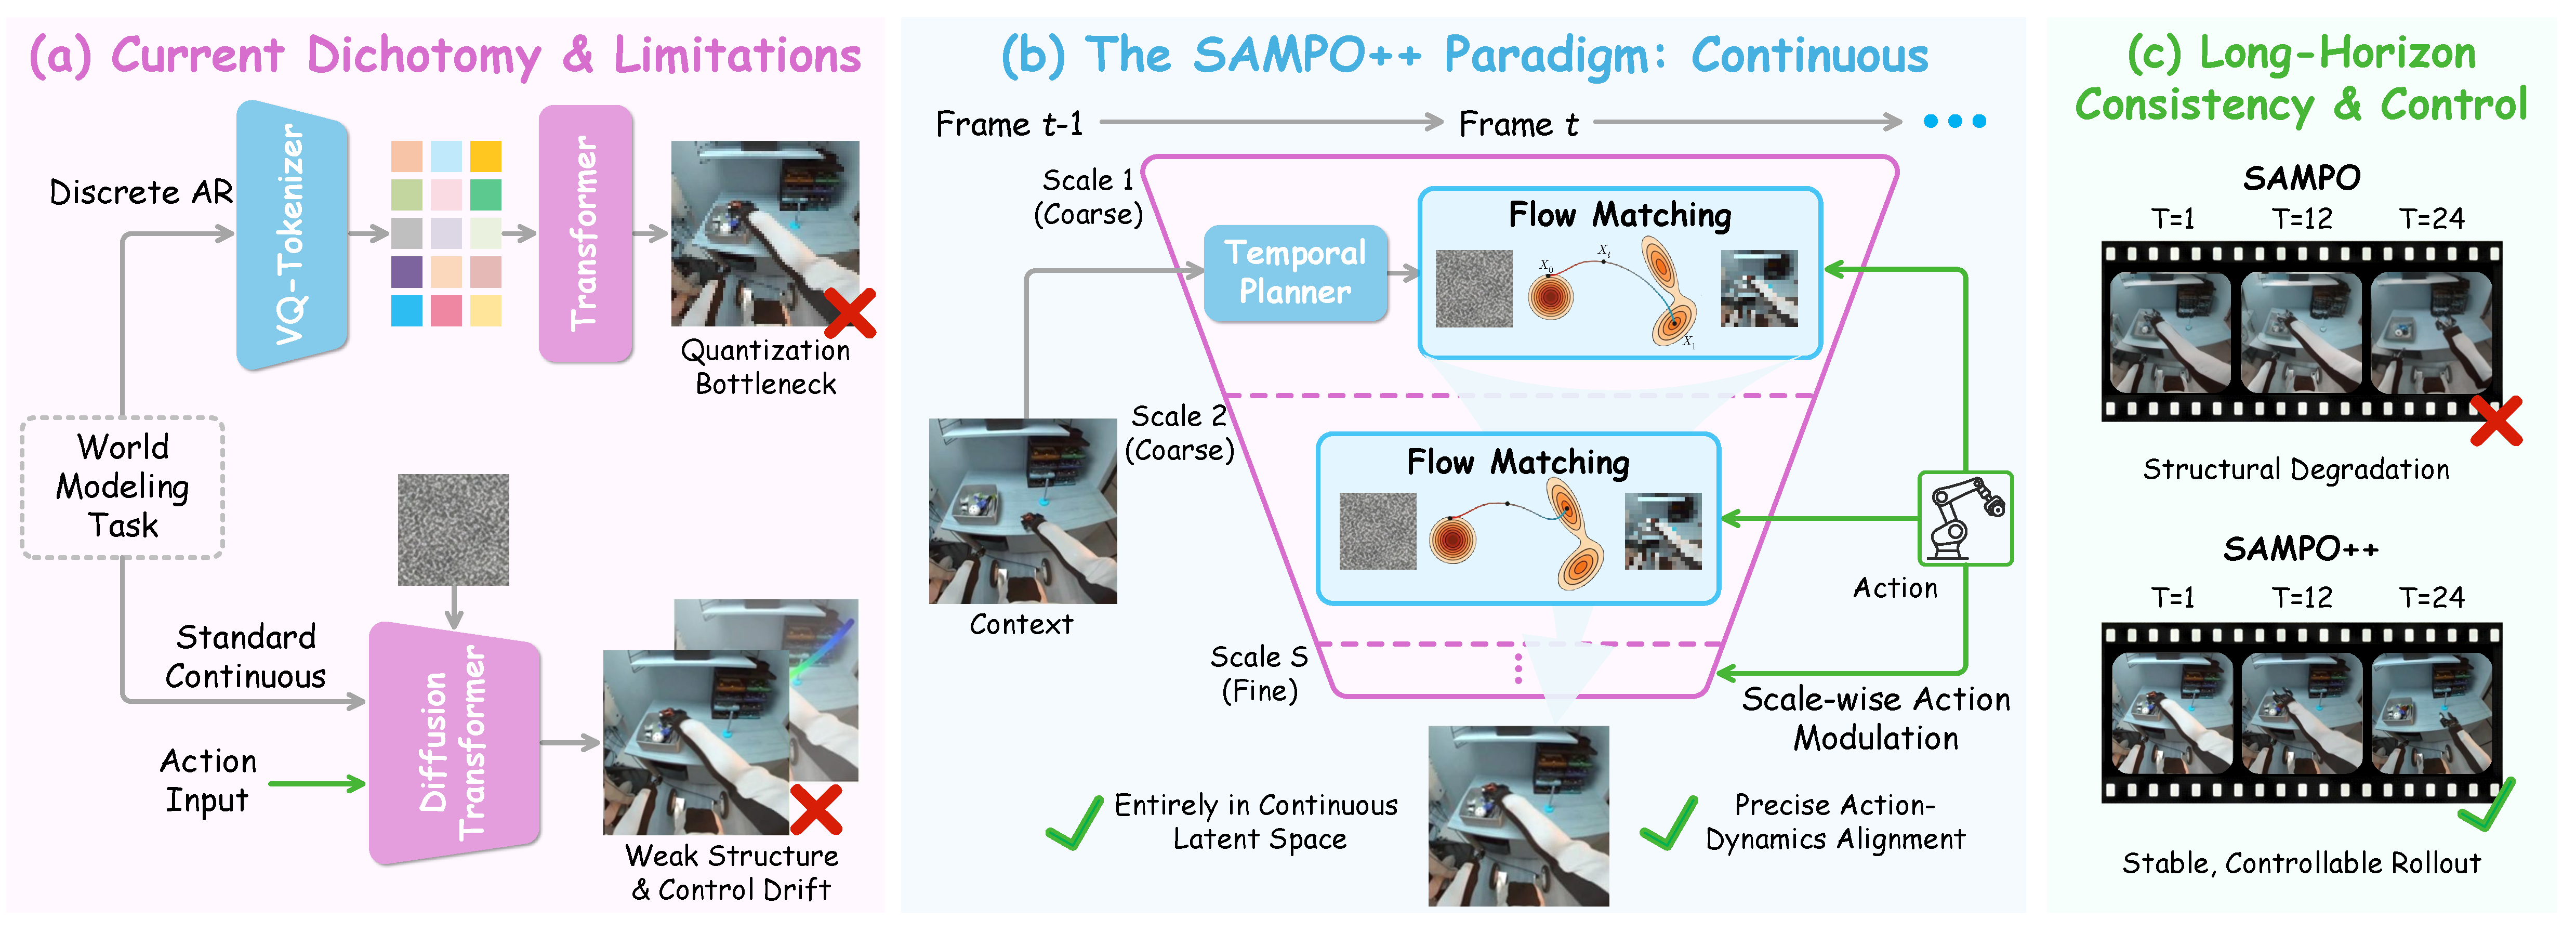
\includegraphics[width=\linewidth]{fig/fig1.pdf}
    \caption{\textbf{Conceptual comparison and framework overview.} 
    \textbf{(a) The prevailing dichotomy:} Existing world models confront a structural trade-off: discrete AR models are hindered by intrinsic quantization artifacts, whereas standard continuous models are restricted to fixed-length synthesis, thereby precluding interactive long-horizon generation.
    \textbf{(b) The SAMPO++ solution:} Our framework resolves this dilemma via a unified ``Predict-then-Refine'' paradigm, synergizing temporal autoregression with scale-wise flow matching directly on a continuous latent manifold. Crucially, it integrates Action-adaptive Dynamics Modulation to enforce precise, frequency-aware control.
    \textbf{(c) Performance:} Consequently, SAMPO++ demonstrates superior long-term physical coherence and action fidelity, effectively mitigating the degradation observed in state-of-the-art baselines.}   
    \label{fig1}
\end{figure*}

As illustrated in Figure~\ref{fig1}\textcolor{blue}{(a)}, this work postulates that the prevailing dichotomy between discrete causal reasoning and continuous high-fidelity generation constitutes a structural constraint rather than a fundamental theoretical limitation. We hypothesize that the hierarchical advantages of scale-wise progression, as demonstrated in recent frameworks~\cite{wang2025sampo,tian2024visual,li2024autoregressive}, can be fully preserved while systematically transcending the representational restrictions inherent to discrete tokenization.
To actualize this conceptual synergy, we propose SAMPO++ (see Figure~\ref{fig1}\textcolor{blue}{(b)}), a unified world modeling framework that seamlessly integrates temporal autoregressive modeling with scale-wise flow matching. Diverging from prior discrete approaches constrained by token indices, SAMPO++ operates entirely within a continuous latent manifold. The video generation process is formulated as a ``Predict-then-Refine'' paradigm: a temporal autoregressive backbone first predicts the coarse conditional distribution, establishing a robust structural prior. Subsequently, a scale-wise flow matching generator~\cite{ren2024flowar, ma2024sit} progressively synthesizes continuous latent features from noise based on this prior. This hybrid architecture effectively synergizes the long-horizon planning capabilities of autoregressive transformers with the resolution-independent synthesis potential of continuous flow matching.

Realizing this unified architecture entails three core technical innovations:

First, to realize unified scale-wise generative modeling, we replace the conventional ``next-token prediction'' objective with a next-scale flow conditional prediction objective. This formulation enables the synthesis of environmental dynamics in a coarse-to-fine manner, prioritizing global motion dynamics before resolving high-frequency textural details. This hierarchical approach effectively incorporates the inductive bias of human perception regarding macro-to-micro visual processing~\cite{denton2015deep}, thereby avoiding the quantization artifacts inherent in discrete modeling.

Second, to achieve precise action-controllability, we introduce an Action-adaptive Dynamics Modulation (ADM) mechanism, effectively overcoming the limitation where existing methods treat action inputs merely as passive conditions. Inspired by advances in pixel-space diffusion~\cite{yu2025pixeldit}, this module injects control signals via scale-aware affine transformations that modulate the feature statistics (mean and variance) of the flow matching layers~\cite{park2019spade, karras2019stylegan2}. Crucially, this modulation is disentangled across scales, allowing actions to distinctly influence global displacements at coarse scales and local deformations at fine scales, yielding a granularity of control previously unattainable.

Third, to ensure long-term spatiotemporal consistency and mitigate the compounding error accumulation inherent to continuous autoregression, we propose a Scale-Aware spacetime Rotary Position Embedding (SA-RoPE). This mechanism establishes a unified 4D positional encoding integrating time, space, and scale dimensions, thereby enforcing strict resolution hierarchy constraints during temporal evolution~\cite{su2024roformer,tian2025pdfactor,yesiltepe2025infinity}. Furthermore, we incorporate an inference-time flow trajectory rectification strategy that leverages optical flow priors to actively rectify latent feature drift and ensure rigorous physical consistency over extended horizons~\cite{teed2020raft, ji2026videoar}.

% To this end, we introduce SAMPO++, a unified world modeling framework integrating temporal autoregression with scale-wise flow matching within a fully continuous latent space. Formulated under a ``Predict-then-Refine'' paradigm, our architecture reconciles structured causal planning with high-fidelity continuous synthesis, thereby circumventing the quantization bottlenecks inherent to prior discrete approaches. 
Extensive empirical validation demonstrates that SAMPO++ establishes a new state-of-the-art across a broad spectrum of dynamic environments. Crucially, not only does our framework achieve unprecedented fidelity in passive video synthesis spanning robotic manipulation (\textit{e.g.}, BAIR~\cite{ebert2017selfBAIR}, RoboNet~\cite{dasari2019robonet}, 1X World Model~\cite{1X_Technologies_1X_World_Model_2024}) and autonomous driving (\textit{e.g.}, Cityscapes~\cite{Cityscapes}, OpenDV-YouTube~\cite{yang2024genad}), but it also serves as a highly reliable neural simulator for downstream control. Specifically, SAMPO++ sets new benchmarks in visual planning with action-conditioned rollouts on the VP$^2$ suite~\cite{tian2023control} and significantly elevates sample efficiency in model-based reinforcement learning (MBRL) within the complex Meta-World environments~\cite{yu2020meta}.
In summary, our main contributions are:
\begin{itemize}
    \item We propose SAMPO++, a unified world modeling architecture that bridges temporal autoregression with scale-wise flow matching, eliminating quantization artifacts while preserving robust causal planning capabilities.
    
    \item We design an Action-adaptive Dynamics Modulation (ADM) mechanism. By dynamically modulating generative flow statistics via scale-aware affine transformations, we achieve precise responsiveness.
        
    \item We introduce a Scale-Aware spacetime RoPE and a predictive flow rectification strategy, solving the degradation problem in long-horizon continuous video prediction.
    
    \item We provide a rigorous evaluation on five large-scale benchmarks covering indoor robotics and outdoor driving scenarios, setting new performance records and validating the scalability of the proposed approach.
\end{itemize}

%%%%%%%%%%%%%%%%%%%%%%%%%%%%%%%%%%%%%%%%%%%%%%%%%%%%%%%%%%%%%%%%%%%%%%%%%%
This paper substantially extends our preliminary conference version~\cite{wang2025sampo} and makes the following new contributions:
\begin{itemize}
    \item Proposing SAMPO++, a unified continuous-space framework merging temporal autoregression with scale-wise flow matching to bypass quantization bottlenecks for high-fidelity synthesis.
    
    \item Introducing Action-adaptive Dynamics Modulation, enabling precise controllability by injecting action signals into flow statistics via scale-aware affine transformations.
    
    \item Integrating Scale-Aware spacetime Rotary Position Embeddings and flow trajectory rectification to enforce long-term physical coherence using spatiotemporal-scale coordinates and optical flow priors.

    \item Conducting additional experiments on Cityscapes~\cite{Cityscapes} and OpenDV dataset~\cite{yang2024genad} and new ablation studies to validate the effectiveness of each component.
\end{itemize}

The remainder of this paper is organized as follows: Section~\ref{Sec2:RelatedWork} reviews related work on generative modeling paradigms and embodied world models. Section~\ref{Sec3:Method} details the proposed unified framework. Section~\ref{Sec4:Experiments} presents comprehensive experimental results and ablation studies. Finally, Section~\ref{Sec5:Conclusion} concludes the paper.


\section{Related Work}
\label{Sec2:RelatedWork}

\subsection{Autoregressive and Scale-wise Visual Generation}
Autoregressive (AR) modeling, fundamentally rooted in the probability chain rule, has long served as a cornerstone of generative AI by decomposing intractable high-dimensional distributions into sequences of conditional probabilities. Early pixel-level paradigms, exemplified by PixelRNN~\cite{van2016pixel} and PixelCNN++~\cite{salimans2017pixelcnn++}, theoretically validated this approach but were practically constrained by prohibitive $O(N)$ sequential complexity and limited receptive fields over flattened sequences. The field witnessed a paradigm shift with the introduction of Vector Quantized Variational Autoencoders (VQ-VAE)~\cite{van2017neural} and VQGAN~\cite{esser2021taming}. By compressing high-resolution visual signals into low-dimensional discrete codebooks, these methods enabled Transformers~\cite{vaswani2017attention} to model long-range dependencies within a computationally feasible latent space. This ``Discrete Tokenization + Transformer'' recipe has since become the gold standard for large-scale synthesis, powering foundational models such as DALL-E~\cite{ramesh2021zero}, VideoGPT~\cite{yan2021videogpt}, and MAGVIT~\cite{yu2023language}. Despite the scalability of latent AR models, the conventional raster-scan ordering (top-left to bottom-right) inherently imposes a unidirectional bias that neglects the 2D spatial locality of visual data. To address this structural limitation, recent works like Visual Autoregressive modeling (VAR)~\cite{tian2024visual} and our preliminary framework SAMPO~\cite{wang2025sampo} pioneered a next-scale prediction paradigm. By reformulating generation as a hierarchical progression from coarse structural maps to fine-grained details, these approaches not only align with the global-to-local nature of human perception but also drastically compress sequence complexity from $O(n^2)$ to $O(\log n)$. Nevertheless, a critical vulnerability persists across this lineage: the reliance on discrete quantization. The discrete codebook acts as a lossy information bottleneck, introducing irreducible quantization artifacts and precluding the precise modeling of continuous physical dynamics, such as fluid turbulence or subtle illumination gradients. SAMPO++ fundamentally transcends this limitation by replacing the discrete tokenizer with a unified continuous flow formulation, thereby enabling infinite-resolution synthesis while retaining the efficient structural planning of scale-wise autoregression.


\subsection{Flow Matching and Continuous Latent Dynamics}
Continuous generative models operate on the principle of transforming a simple prior distribution (\textit{e.g.}, Gaussian) into a complex data distribution. Diffusion Probabilistic Models (DPMs)~\cite{ho2020denoising, song2020score} achieve this by learning to reverse a gradual noising process. While DPMs and Latent Diffusion Models (LDM)~\cite{rombach2022high} have established the benchmark for perceptual quality (\textit{e.g.}, Sora~\cite{liu2024sora}), their stochastic sampling trajectories are typically curved and complex, necessitating extensive discretization steps for high-quality inference. Flow Matching (FM)~\cite{lipman2023flow, liuflow, albergo2025stochastic,wang2025flowram} has emerged as a robust alternative, grounded in the theory of Continuous Normalizing Flows (CNFs). Unlike diffusion, FM objectives facilitate the construction of Conditional Vector Fields (CVFs) that regress linear Optimal Transport (OT) paths between source and target distributions. This formulation yields straighter generation trajectories, significantly faster convergence, and superior stability for ODE solvers. Recent variants, such as Rectified Flow~\cite{liuflow} and SiT~\cite{ma2024sit}, have further optimized this framework utilizing Scalable Interpolant Transformers.

An emerging research direction involves hybridizing AR architectures with continuous objectives to reconcile semantic reasoning with visual generation. Approaches like Transfusion~\cite{zhou2024transfusion} and Show-o~\cite{xie2024show} demonstrate the feasibility of training Transformers on mixed modalities, such as discrete text and continuous image patches. Most relevant to our work is FlowAR~\cite{ren2024flowar}, which applies flow matching to the residual of scale-wise image generation. However, FlowAR remains confined to static imagery, functioning primarily as an image upsampler rather than a dynamic simulator. To address this limitation, SAMPO++ extends hybrid continuous-discrete paradigm into the spatiotemporal domain. By integrating temporal autoregression, our framework explicitly enforces the strict causality essential for world modeling, moving beyond the synthesis of independent high-fidelity frames.


\subsection{Action-Conditioned World Models for Embodied Agents}
The World Model paradigm~\cite{ha2018world} posits that embodied agents utilize internal predictive simulators of the environment to facilitate planning and policy learning. Early RSSM-based instantiations, such as the Dreamer framework~\cite{hafner2019dream, hafner2020dreamerv2, hafner2023dreamerv3}, achieved high sample efficiency for policy optimization but were constrained by low-resolution reconstructions that limited their applicability in fine-grained manipulation tasks. Recent advancements have pivoted toward Generative World Models, employing diffusion or transformer backbones to achieve photorealistic simulation. Systems such as Genie~\cite{bruce2024genie} and GameNGen~\cite{valevski2024diffusion} demonstrate the capability to simulate interactive environments or complex game logic with high fidelity. However, a fundamental divergence exists regarding the prediction domain. Joint Embedding Predictive Architectures (JEPA)~\cite{assran2025v,assran2023self} operate in abstract feature spaces to mitigate stochasticity, whereas full generative approaches~\cite{liu2024sora, alonso2024diffusion} synthesize observable data to ensure interpretability. Our framework aligns with the latter strategy but operates within a continuous latent manifold to balance semantic compactness with visual reconstructability.

Despite improved visual fidelity, precise action-controllability and long-term physical consistency remain unresolved challenges. Existing methods generally treat action inputs as passive conditions via embedding concatenation or cross-attention~\cite{zhang2023adding, mou2024t2i}, often resulting in control drift where visual dynamics decouple from input actions over extended horizons. Recent investigations indicate that modulating normalization statistics, as explored in pixel-space diffusion~\cite{yu2025pixeldit}, provides superior structural control compared to standard attention mechanisms. Furthermore, while specialized positional encodings effectively mitigate coordinate drift in discrete autoregressive models~\cite{han2024infinity}, analogous mechanisms for continuous flow fields are currently absent. To address these limitations, we introduce a scale-aware action modulation mechanism for frequency-specific control and formulate a unified spatiotemporal positional encoding to strictly enforce physical consistency during long-term prediction.


\section{Methodology}
\label{Sec3:Method}

\subsection{Preliminaries: Next-scale Prediction}
\label{subsec:preliminaries}
We formulate each video frame as a hierarchical pyramid of latent grids, adopting the structural paradigm introduced in recent scale-wise generative frameworks~\cite{tian2024visual, wang2025sampo}. Let $S$ denote the total number of spatial scales, indexed from the coarsest $s=1$ to the finest $s=S$. For a video frame at time step $t$, its multi-scale continuous latent representation is defined as:
\begin{equation}
\label{eq:pyramid_latent}
\boldsymbol{z}_t = \{\boldsymbol{z}_t^{s}\}_{s=1}^{S}, \;\; \boldsymbol{z}_t^{s} \in \mathbb{R}^{H_s \times W_s \times C_s}
\end{equation}
where $\boldsymbol{z}_t^{s}$ denotes the latent grid at scale $s$, with $(H_s, W_s)$ and $C_s$ denoting the spatial resolution and channel dimension, respectively. Unlike traditional autoregressive approaches~\cite{parkerholder2024genie2,wu2024ivideogpt,wu2024controlmllm} that flatten spatial features into a 1D raster-scan sequence, this representation inherently preserves the 2D spatial topology at each scale.

Next-scale Prediction factorizes intra-frame generation across the scale hierarchy~\cite{tian2024visual}. Given a conditioning signal $\boldsymbol{h}_t$, which encapsulates the temporal context and control inputs, the joint distribution of the latent pyramid is factorized as:
\begin{equation}
\label{eq:nextscale_factorization}
p(\boldsymbol{z}_t \mid \boldsymbol{h}_t) = \prod_{s=1}^{S} p(\boldsymbol{z}_t^{s} \mid \boldsymbol{z}_t^{<s}, \boldsymbol{h}_t), \;\; \boldsymbol{z}_t^{<s} \triangleq \{\boldsymbol{z}_t^{k}\}_{k=1}^{s-1}.
\end{equation}
where $\boldsymbol{z}_t^{<s}$ represents the collection of all coarser scales. Eq.~\eqref{eq:nextscale_factorization} implies that each feature map $\boldsymbol{z}_t^{s}$ is generated holistically conditioned on its preceding coarser structural priors $\boldsymbol{z}_t^{<s}$ and the historical context $\boldsymbol{h}_t$.
Consequently, it circumvents lengthy token-level dependencies, allowing for the integration of highly parallelizable continuous transport models.

In  action-conditioned world modeling, the conditioning variable $\boldsymbol{h}_t$ summarizes the causal dynamics up to the current state. We formalize this temporal dependency as:
\begin{equation}
\label{eq:temporal_context_def}
\boldsymbol{h}_t = \Phi(\boldsymbol{z}_{<t}, \boldsymbol{a}_{<t}), \;\; \boldsymbol{z}_{<t} \triangleq \{\boldsymbol{z}_\tau\}_{\tau < t},
\end{equation}
where $\boldsymbol{z}_{<t}$ denotes the past latent trajectory, $\boldsymbol{a}_{<t}$ indicates the sequence of executed actions, and $\Phi(\cdot)$ represents a causal temporal mapping (\textit{e.g.}, a decoder-only Transformer). Under this mathematical framework, next-scale prediction functions as a versatile interface, seamlessly linking temporal causality with continuous intra-frame synthesis.


\subsection{Problem Statement}
\label{subsec:problem_statement}
We focus on the problem of learning an action-conditioned world model to enable interactive environment simulation. Formally, the environment is modeled as a Partially Observable Markov Decision Process (POMDP), characterized by the tuple $\mathcal{M}=(\mathcal{S}, \mathcal{O}, \mathcal{A}, \mathcal{T}, \mathcal{R}, \gamma)$. At each time step $t$, the agent perceives a partial observation $\boldsymbol{o}_t \in \mathcal{O}$, executes an action $\boldsymbol{a}_t \in \mathcal{A}$, and receives a corresponding reward $r_t = \mathcal{R}(\boldsymbol{s}_t, \boldsymbol{a}_t)$ based on the unobserved true state $\boldsymbol{s}_t \in \mathcal{S}$. The core capability of a world model lies in approximating these underlying transition dynamics to support downstream planning and policy optimization. Specifically, we seek to model the joint distribution over future trajectories, conditioned on historical observations and a sequence of candidate actions:
\begin{equation}
\label{eq:wm_goal}
p(\boldsymbol{o}_{t+1:t+H}, r_{t+1:t+H} \mid \boldsymbol{o}_{1:t}, \boldsymbol{a}_{1:t+H}),
\end{equation}
where $H$ denotes the prediction horizon. 

To ensure scalability while maintaining high visual fidelity, we operate within the continuous latent space defined in Sec.~\ref{subsec:preliminaries}. Let $\boldsymbol{z}_t = \mathcal{E}(\boldsymbol{o}_t)$ denote the latent pyramid extracted by a continuous encoder $\mathcal{E}$ (following the structure in Eq.~\eqref{eq:pyramid_latent}), and let $\hat{\boldsymbol{o}}_t = \mathcal{D}(\boldsymbol{z}_t)$ represent the reconstructed observation. Consequently, our objective is to learn a parametric model $p_\theta$ that generates the future latent trajectory given a context of length $T_c$ and an action plan $\boldsymbol{a}_{1:T}$:
\begin{equation}
\label{eq:rollout_obj_latent}
p_\theta(\boldsymbol{z}_{T_c+1:T}, r_{T_c+1:T} \mid \boldsymbol{z}_{1:T_c}, \boldsymbol{a}_{1:T}).
\end{equation}
This formulation enables the agent to perform interactive rollouts and evaluate candidate action sequences to optimize decision-making. The proposed unified framework, which realizes this objective through scale-wise flow matching, is presented in Section~\ref{Sec3:UnifiedFramework}.

%%%%%%%%%%%%%%%%%%%%%%%%%%%%%%%%%%%%%%%%%%%%%%%%%%%%%%%%%%%%%%%%%%%%%%%%%%%%%%%%%%%%  
\begin{figure*}
    \centering
    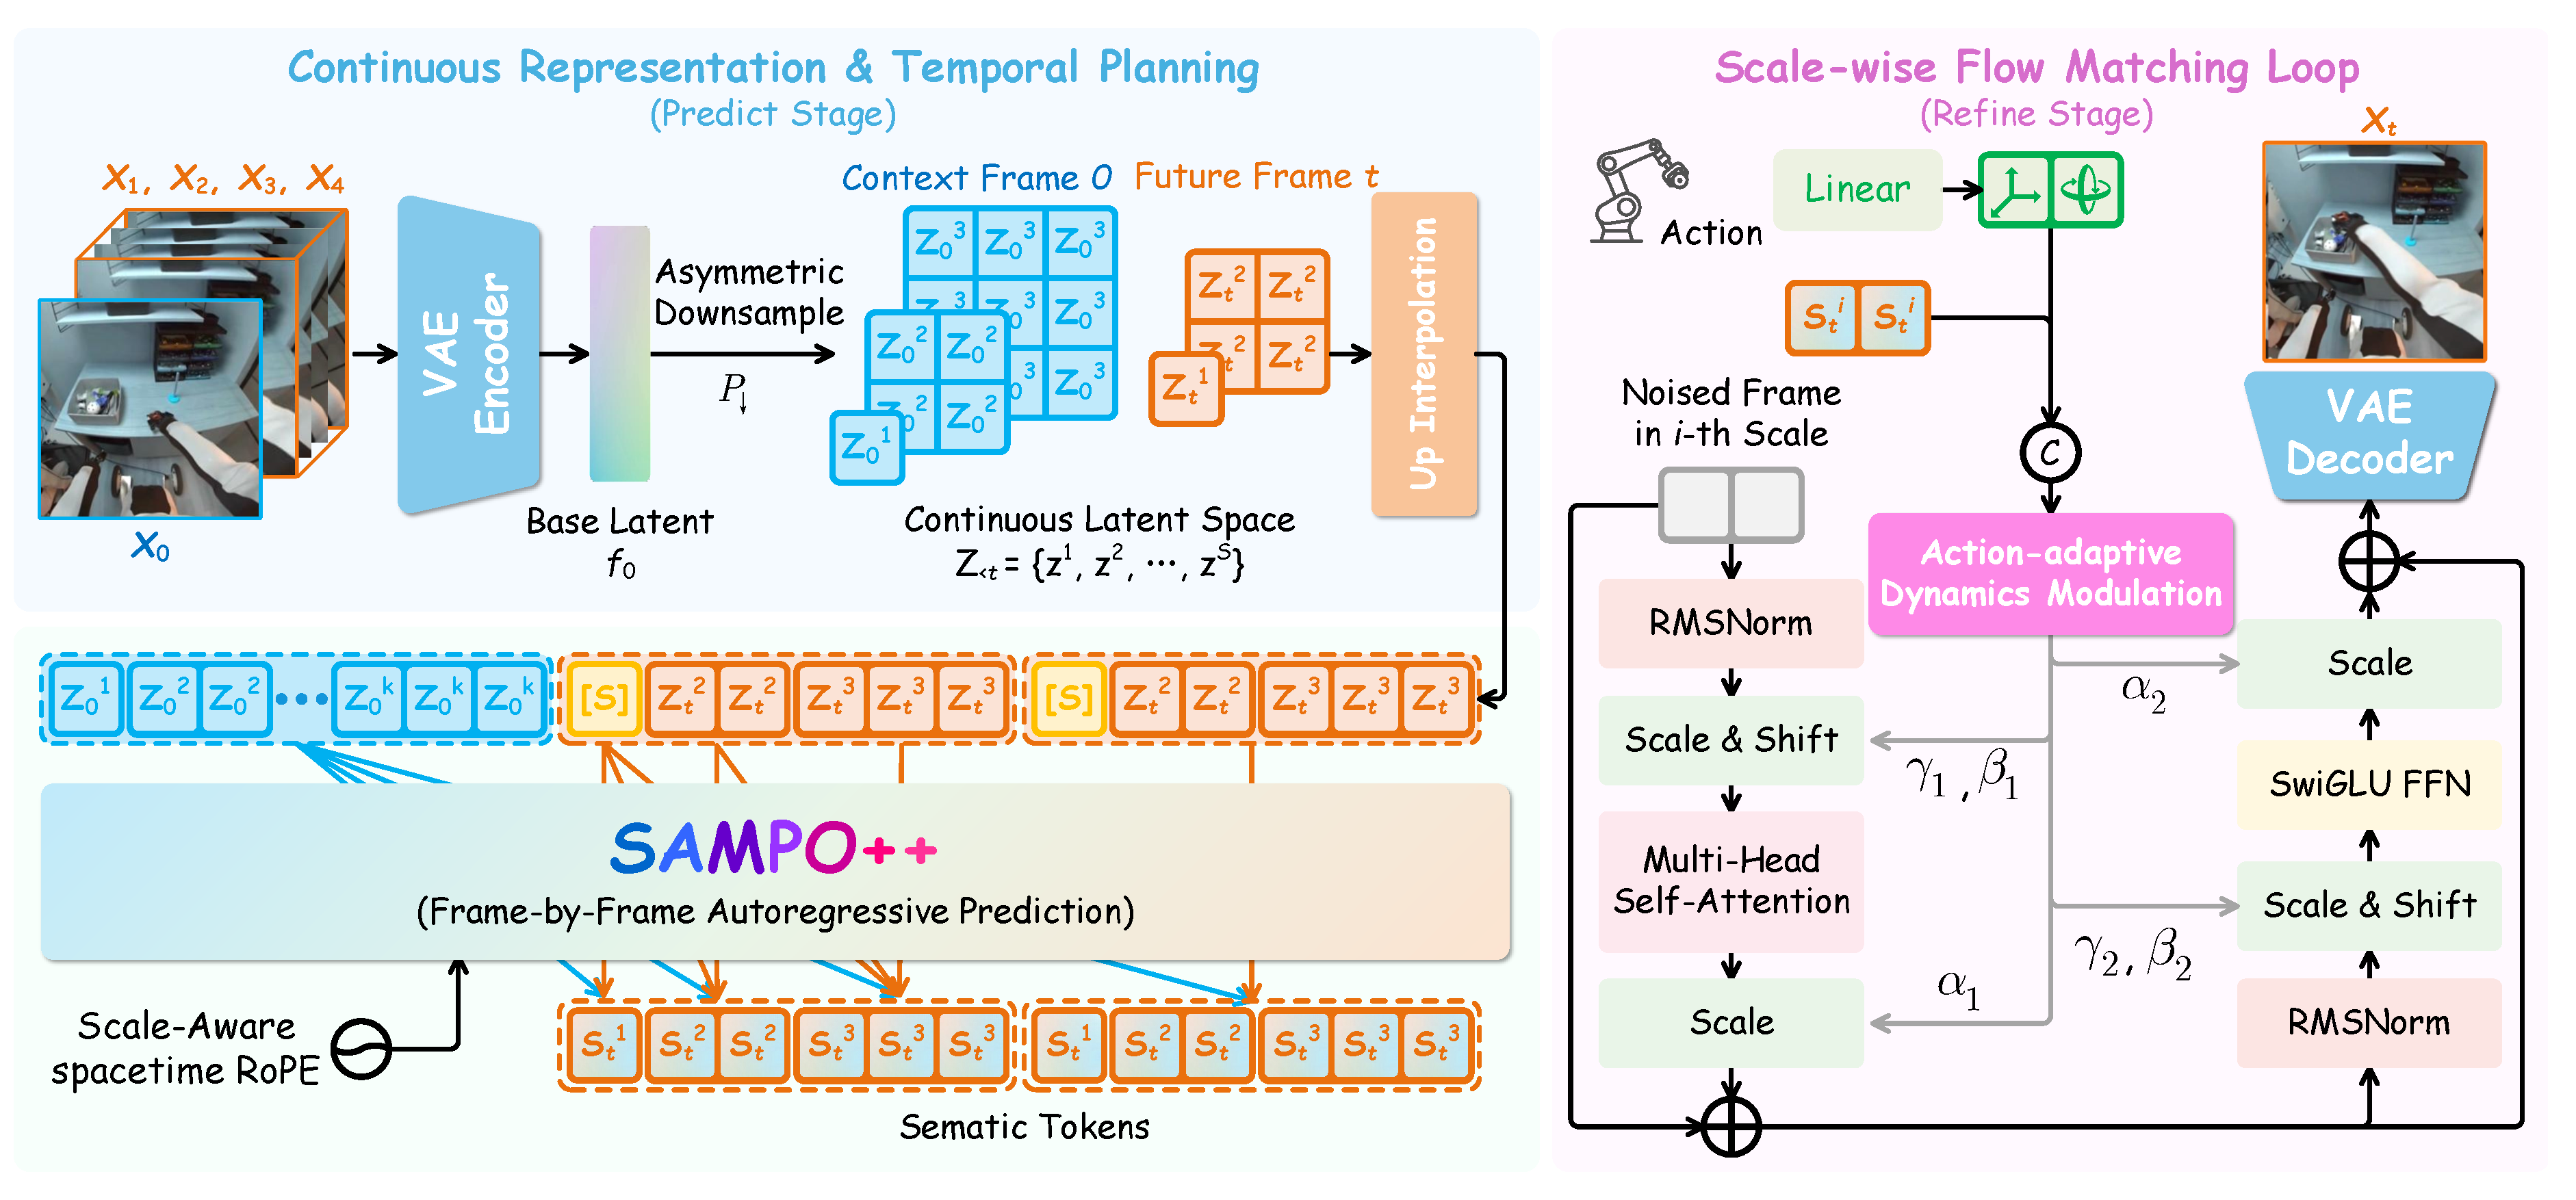
\includegraphics[width=\linewidth]{fig/fig2.pdf}
    \caption{\textbf{SAMPO++ overview}. 
    \textbf{A. Predict Stage:} Both historical context and target future frames are encoded into continuous latent pyramids via a pre-trained VAE followed by asymmetric downsampling. An autoregressive temporal planner aggregates historical features to generate multi-scale semantic representations $\{S^1, S^2, \dots\}$.
    \textbf{B. Refine Stage:} At each scale, a conditional flow matching network (parameterized as a Scale-aware DiT) predicts the velocity field required to transport noise to the target data distribution at a random timestep $t$ (timestep conditioning is omitted for simplicity). This generation process is explicitly conditioned on the semantic representations and control signals via the Action-adaptive Modulation (ADM) mechanism.}
    \label{fig2:pipline}
    % \vspace{-2ex}
\end{figure*}
%%%%%%%%%%%%%%%%%%%%%%%%%%%%%%%%%%%%%%%%%%%%%%%%%%%%%%%%%%%%%%%%%%%%%%%%%%%%%%%%%%%%  


\subsection{Continuous Pyramidal Latent Representation}
\label{Sec3:Representation}
To enable high-fidelity video generation capable of capturing subtle dynamic variations, such as fluid turbulence and lighting gradients, we fundamentally depart from the discrete tokenization paradigm prevalent in prior autoregressive world models~\cite{esser2021taming,wang2025sampo}. Although discrete codebooks facilitate categorical distribution modeling, they impose a non-differentiable quantization bottleneck. This bottleneck inherently limits the upper bound of reconstructive quality and induces high-frequency flickering artifacts~\cite{yu2023language}.

To circumvent this, we construct a continuous pyramidal latent representation to map visual observations onto a smooth, hierarchical, and differentiable manifold. 
Let $\boldsymbol{x}_t \in \mathbb{R}^{H \times W \times 3}$ denote the raw video frame at time step $t$. Rather than relying on off-the-shelf image encoders, we adopt the Vision foundation model Aligned Variational AutoEncoder (VA-VAE) framework~\cite{yao2025reconstruction}. By leveraging rigorous in-domain pre-training, we explicitly align the empirical visual distribution with our continuous manifold. This domain-aligned encoder $\mathcal{E}$ is subsequently deployed to extract a robust base latent feature map $\boldsymbol{f}_t^0 \in \mathbb{R}^{h \times w \times c}$. 
Crucially, we bypass the quantization operation entirely, retaining the continuous latent distributions parameterized by their moments for downstream modeling.

To establish the multi-scale hierarchy required for coarse-to-fine generation, we introduce a recursive downsampling operator $\mathcal{P}_{\downarrow}$, inspired by Laplacian pyramids~\cite{denton2015deep}. The resulting latent pyramid $\mathcal{Z}_t = \{ \boldsymbol{z}_t^1, \boldsymbol{z}_t^2, \dots, \boldsymbol{z}_t^S \}$ is defined as:
\begin{equation}
    \boldsymbol{z}_t^S = \boldsymbol{f}_t^0, \;\; \boldsymbol{z}_t^{s-1} = \mathcal{P}_{\downarrow}(\boldsymbol{z}_t^s), \;\; \text{for } s = S, \dots, 2,
\end{equation}
where $S$ denotes the total number of scales. The scale $s=S$ corresponds to the finest resolution containing intricate texture details, while $s=1$ represents the coarsest resolution (\textit{e.g.}, $1 \times 1$ or $2 \times 2$) describing the global semantic layout. Mathematically, the feature map at scale $s$ lies in the space $\mathbb{R}^{h_s \times w_s \times c}$, where $h_s = h / 2^{S-s}$ and $w_s = w / 2^{S-s}$.

Adopting this continuous framework yields two significant theoretical advantages over discrete tokenization. First, it inherently preserves manifold continuity. By operating within $\mathbb{R}^n$, the representation space remains unfragmented, which allows the generative model to approximate the true data distribution with arbitrary precision. This effectively avoids the quantization error inherent in discrete approaches, wherein the true latent state falls between two codebook centroids. Second, it ensures compatibility with gradient-based dynamics. Continuous vectors naturally align with the Ordinary Differential Equation (ODE) framework utilized in Flow Matching~\cite{chen2018neural, lipman2023flow}. This alignment enables us to model the transition between scales as a smooth trajectory integration problem, in stark contrast to the categorical classification tasks required by discrete tokenization.

\subsection{Unified Temporal Autoregressive with Scale-wise Flow Matching}
\label{Sec3:UnifiedFramework}
The core premise of SAMPO++ lies in disentangling the complexity of world modeling into two orthogonal axes: Time and Resolution. We observe that relying solely on autoregression~\cite{esser2021taming,wu2024ivideogpt,brown2020language,yan2021videogpt} is computationally prohibitive for high-dimensional visual data. Conversely, relying exclusively on diffusion or flow models~\cite{blattmann2023stable,zhu2024sora,lipman2023flow,dao2023flow} fails to capture the explicit causal reasoning required for effective planning.
To bridge this gap, we introduce a hybrid probabilistic framework that decomposes the joint distribution $p(\boldsymbol{z}_{1:T})$ into an Inter-frame Temporal Autoregressive component responsible for causal planning, and an Intra-frame Scale-wise Flow component dedicated to high-fidelity rendering. This architecture embodies a "Predict-then-Refine" paradigm, which is mathematically formulated as:
\begin{equation}
    p_\theta(\boldsymbol{z}_{1:T} | \boldsymbol{a}_{1:T}) = \prod_{t=1}^{T} \underbrace{p_\theta(\boldsymbol{h}_t | \boldsymbol{z}_{<t}, \boldsymbol{a}_{<t})}_{\text{Inter-frame Planning}} \cdot \prod_{s=1}^{S} \underbrace{p_\theta(\boldsymbol{z}_t^s | \boldsymbol{z}_t^{<s}, \boldsymbol{h}_t)}_{\text{Intra-frame Refinement}}.
\end{equation}
The following subsections elaborate on these components and their synergistic integration.

\noindent \textit{\textbf{1) Inter-frame Temporal Autoregression: The Causal Planner.}}
The fundamental objective of the temporal module is to model the causal evolution of the environment's state dynamics. Rather than predicting raw pixels or stochastic high-frequency details, which are inherently intractable to model autoregressively~\cite{van2016pixel, yan2021videogpt}, this module is dedicated to inferring a Temporal Context Vector $\boldsymbol{h}_t$. This vector acts as a structural prior, encapsulating both the deterministic physics and the semantic intent governing the subsequent frame.

As illustrated in the predict stage of Figure~\ref{fig2:pipline}, we instantiate this module utilizing a scalable causal transformer backbone~\cite{tian2024visual}, denoted as $\mathcal{T}_{\text{time}}$. This network is composed of stacked decoder-only transformer blocks and operates strictly on the sequence of historical finest-scale latents. Defining the history horizon as $\mathcal{H}_{<t} = \{ (\boldsymbol{z}_{1}^S, \boldsymbol{a}_{1}), \dots, (\boldsymbol{z}_{t-1}^S, \boldsymbol{a}_{t-1}) \}$, the temporal forward pass is formulated as:
\begin{equation}
    \boldsymbol{h}_t = \mathcal{T}_{\text{time}}(\text{Embed}(\mathcal{H}_{<t}); \theta_{\text{AR}}),
\end{equation}
where $\boldsymbol{h}_t \in \mathbb{R}^{D}$ is a dense vector acting as a global structural prior for time step $t$.

Crucially, this formulation distinguishes our approach from standard video transformers~\cite{yan2021videogpt, rakhimov2020latent} in two key aspects. First, regarding latent-space operation, the planner processes the highly compressed continuous latent space $\boldsymbol{z}^S$ instead of raw pixels. This design effectively reduces the spatial sequence length by orders of magnitude, thereby enabling computationally efficient long-horizon reasoning—a strategy validated in latent diffusion frameworks~\cite{rombach2022high}. Second, concerning the role of conditioning, the output $\boldsymbol{h}_t$ serves not as the generated frame itself but as an abstract condition for the subsequent generative flow. By relieving the autoregressive module from the burden of synthesizing high-frequency noise, we allow the planner to focus strictly on maintaining temporal consistency and object permanence.

\noindent \textit{\textbf{2) Intra-frame Scale-wise Flow: The Continuous Renderer.}}
Guided by the temporal plan $\boldsymbol{h}_t$ and the coarser structural priors $\boldsymbol{z}_t^{<s}$, the objective of the Intra-frame module is to synthesize the detailed feature map $\boldsymbol{z}_t^s$ at the current scale $s$. We leverage Conditional Flow Matching (CFM), a simulation-free approach for training Continuous Normalizing Flows (CNFs)~\cite{lipman2023flow, albergo2025stochastic, dao2023flow}, to model the complex transition from a tractable noise distribution to the data distribution.

We ground our generative modeling in the framework of probability flow Ordinary Differential Equations (ODEs). Specifically, we define a time-dependent probability density path $p_\tau(\boldsymbol{x})$, where $\tau \in [0, 1]$ denotes the flow time, a variable distinct from the video timestamp $t$. The generation process entails solving an ODE that integrates from Gaussian noise $\boldsymbol{x}_0 \sim \mathcal{N}(\boldsymbol{0}, \boldsymbol{I})$ to the target data sample $\boldsymbol{x}_1 = \boldsymbol{z}_t^s$:
\begin{equation}
    d\boldsymbol{x}_\tau = v_\theta(\boldsymbol{x}_\tau, \tau; \text{cond}_{t,s}) \, d\tau,
\end{equation}
where $v_\theta$ represents a neural velocity field parameterized by a Diffusion Transformer~\cite{peebles2023scalable, yao2025reconstruction}, and $\text{cond}_{t,s} = \{ \boldsymbol{z}_t^{<s}, \boldsymbol{h}_t \}$ denotes the composite conditioning signal.

To facilitate efficient and stable sampling, we supervise this model by enforcing an Optimal Transport (OT) conditional vector field~\cite{lipman2023flow}. By minimizing transport cost, this method establishes straight-line trajectories between the noise distribution and the data distribution~\cite{liuflow}. The target vector field is defined as $u_\tau(\boldsymbol{x}|\boldsymbol{x}_1, \boldsymbol{x}_0) = \boldsymbol{x}_1 - \boldsymbol{x}_0$, leading to the following regression objective:
\begin{equation}
    \mathcal{L}_{\text{Flow}} = \mathbb{E}_{\tau, \boldsymbol{x}_0, \boldsymbol{x}_1} \left[ || v_\theta(\psi_\tau(\boldsymbol{x}_0, \boldsymbol{x}_1), \tau; \text{cond}_{t,s}) - (\boldsymbol{x}_1 - \boldsymbol{x}_0) ||^2 \right],
\end{equation}
where $\psi_\tau(\boldsymbol{x}_0, \boldsymbol{x}_1) = (1-\tau)\boldsymbol{x}_0 + \tau\boldsymbol{x}_1$ represents the linear interpolation state.
To instantiate the velocity field $v_\theta$, we augment the DiT block by replacing LayerNorm with RMSNorm and applying 2D RoPE in all attention layers~\cite{yao2025reconstruction}. Within this augmented architecture, we employ a highly effective dual-injection strategy to incorporate the multi-source conditions. First, for spatial and contextual guidance, the coarser latent $\boldsymbol{z}_t^{<s}$ and the temporal plan $\boldsymbol{h}_t$ are upsampled (if necessary) and strictly concatenated with the noisy state $\boldsymbol{x}_\tau$ along the channel dimension, thereby bounding the velocity field within the established structural envelope. Second, to enforce precise controllability, the action signal $\boldsymbol{a}_t$ is actively injected into the intermediate features via our proposed Action-adaptive Dynamics Modulation (ADM) mechanism. This unified architectural choice ensures that the generated microscopic details, including motion blur and subtle lighting variations, remain strictly coherent with the macroscopic physical evolution predicted by the temporal planner.

By recursively applying this optimal transport process from scale $s=1$ to $S$, SAMPO++ synthesizes high-fidelity frames that are simultaneously physically grounded (governed by $\boldsymbol{h}_t$ and $\boldsymbol{a}_t$) and structurally coherent (guided by $\boldsymbol{z}_t^{<s}$).

\begin{figure}
    \centering
    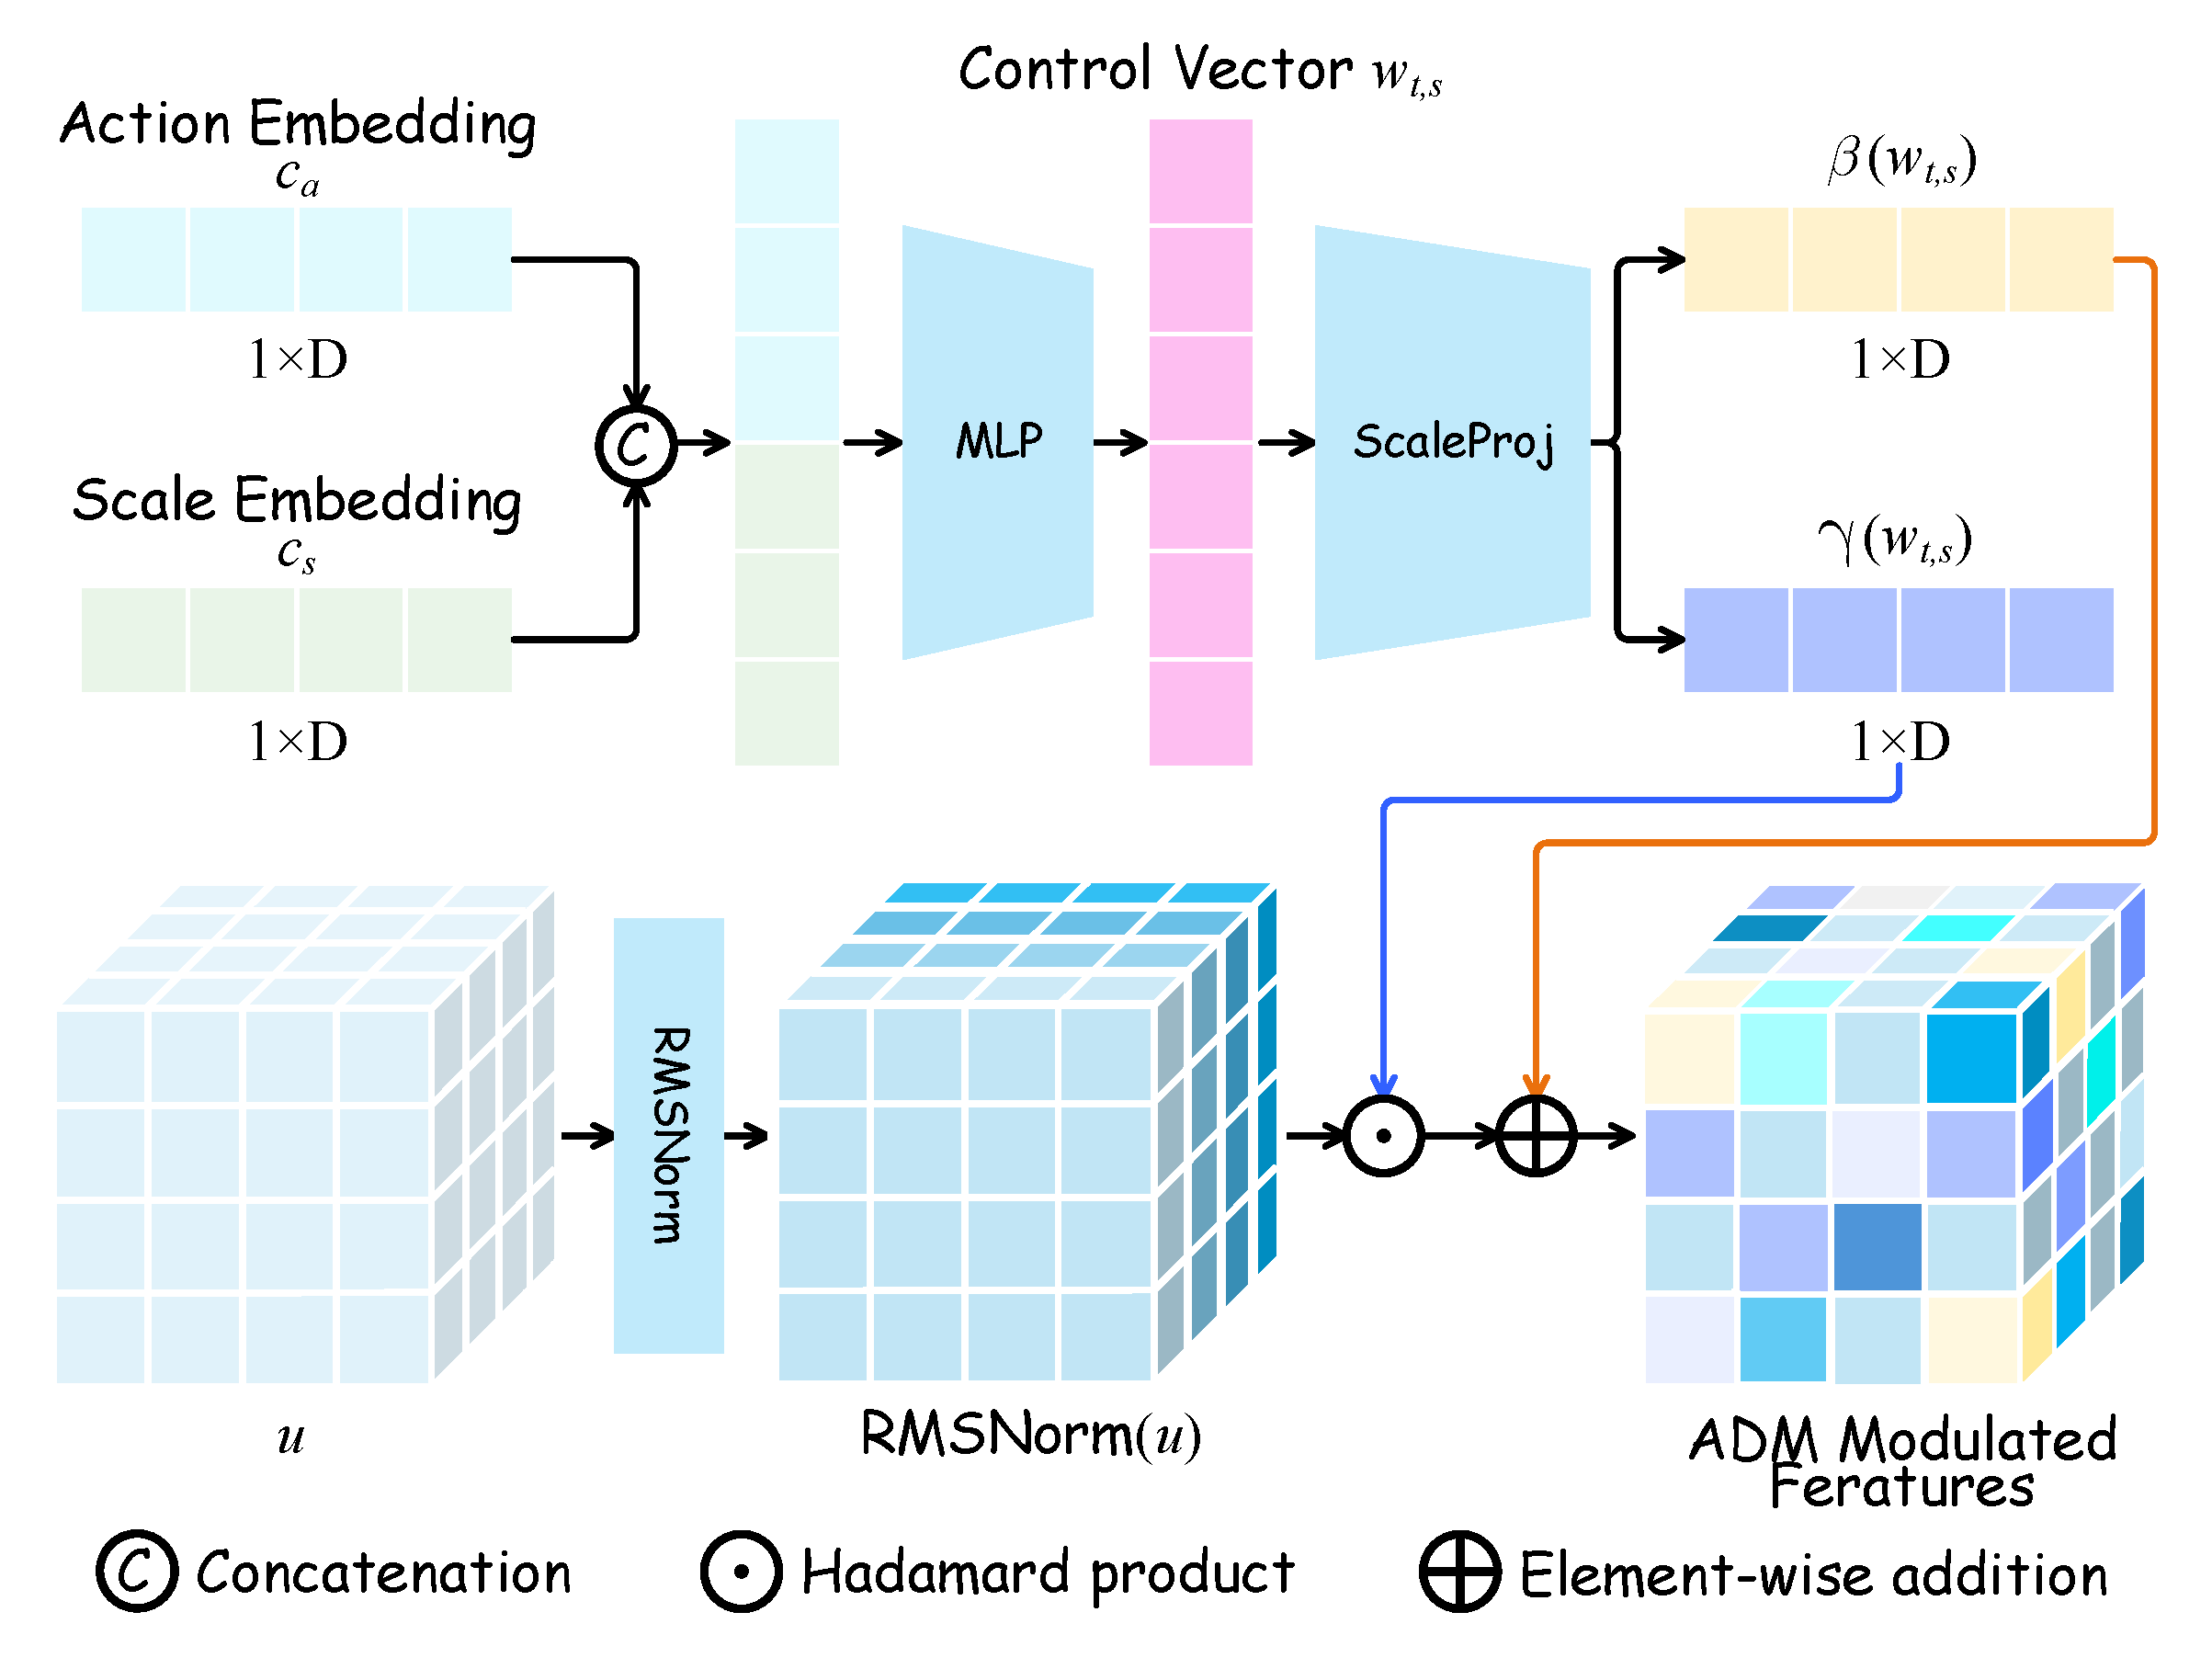
\includegraphics[width=1.0\linewidth]{fig/fig_ADM.pdf}
    \caption{\textbf{Action-adaptive Dynamics Modulation (ADM).} ADM explicitly alters the generative dynamics by modulating intermediate feature statistics. It fuses action and scale embeddings to regress affine parameters ($\boldsymbol{\gamma}$, $\boldsymbol{\beta}$).}
    \label{fig:fig_ADM}
    \vspace{-1ex}
\end{figure}

\subsection{Action-adaptive Dynamics Modulation}
\label{Sec3:ActionModulation}
Existing approaches typically treat actions $\boldsymbol{a}_t$ merely as passive tokens via concatenation or cross-attention~\cite{mou2024t2i, wang2025sampo}. This passive injection is inadequate for physics-based simulation because it fails to explicitly modulate the underlying generative vector field. Furthermore, these signals easily attenuate across deep layers, exacerbating the severe ``action forgetting'' phenomenon.

In response, we propose Action-adaptive Dynamics Modulation (ADM), as illustrated in Figure~\ref{fig:fig_ADM}. This mechanism systematically integrates adaptive normalization principles~\cite{karras2019stylegan2, park2019semantic, yu2025pixeldit} into the flow matching paradigm. Our core insight is that actions should function as global system parameters that actively and directly modulate the intermediate feature statistics of the network. Crucially, we posit that this modulation must be intrinsically scale-aware: microscopic actions (\textit{e.g.}, ``gripper close'') induce localized, high-frequency deformations, whereas macroscopic actions (\textit{e.g.}, ``move forward'') govern low-frequency global displacements. 

We embed ADM directly within the augmented Transformer blocks~\cite{yao2025reconstruction} of our Flow Matching network. For a specific architectural scale $s$ and timestep $t$, we first synthesize a scale-aware control vector $\boldsymbol{w}_{t,s}$ by fusing the time-dependent action embedding $\boldsymbol{c}_a$ with a learnable scale embedding $\boldsymbol{c}_s$:
\begin{equation}
    \boldsymbol{w}_{t,s} = \text{MLP}([ \boldsymbol{c}_a, \boldsymbol{c}_s ]),
\end{equation}
where $[\cdot, \cdot]$ denotes channel-wise concatenation. This intermediate representation is subsequently projected to regress the scale and shift parameters, $\boldsymbol{\gamma}$ and $\boldsymbol{\beta}$, for affine transformation:
\begin{equation}
    \boldsymbol{\gamma}(\boldsymbol{w}_{t,s}), \boldsymbol{\beta}(\boldsymbol{w}_{t,s}) = \text{ScaleProj}(\boldsymbol{w}_{t,s}).
\end{equation}

Within each Transformer block, this active modulation is applied to the intermediate latent feature representation $\boldsymbol{u}$ prior to the self-attention and Feed-Forward Network (FFN) modules. Consistent with our architectural modifications detailed in Section~\ref{Sec3:UnifiedFramework}, we employ RMSNorm to stabilize the continuous flow integration:
\begin{equation}
    \text{ADM}(\boldsymbol{u}, \boldsymbol{a}_t, s) = (\boldsymbol{1} + \boldsymbol{\gamma}_{t,s}) \odot \text{RMSNorm}(\boldsymbol{u}) + \boldsymbol{\beta}_{t,s}.
\end{equation}

Conceptually, this formulation establishes a more mathematically principled integration of control signals into the generation dynamics. In Flow Matching, the neural network parameterizes the velocity field of the probability flow ODE. By modulating the activation statistics via $\boldsymbol{\gamma}$ and $\boldsymbol{\beta}$, ADM continuously applies an action-conditioned affine transformation to the latent manifold. This topological constraint ensures that the action signal imposes a strong, persistent inductive bias along the entire generative trajectory and across all network depths, thereby effectively eradicating action forgetting and yielding superior kinematic control fidelity compared to standard passive conditioning.


\begin{figure}
    \centering
    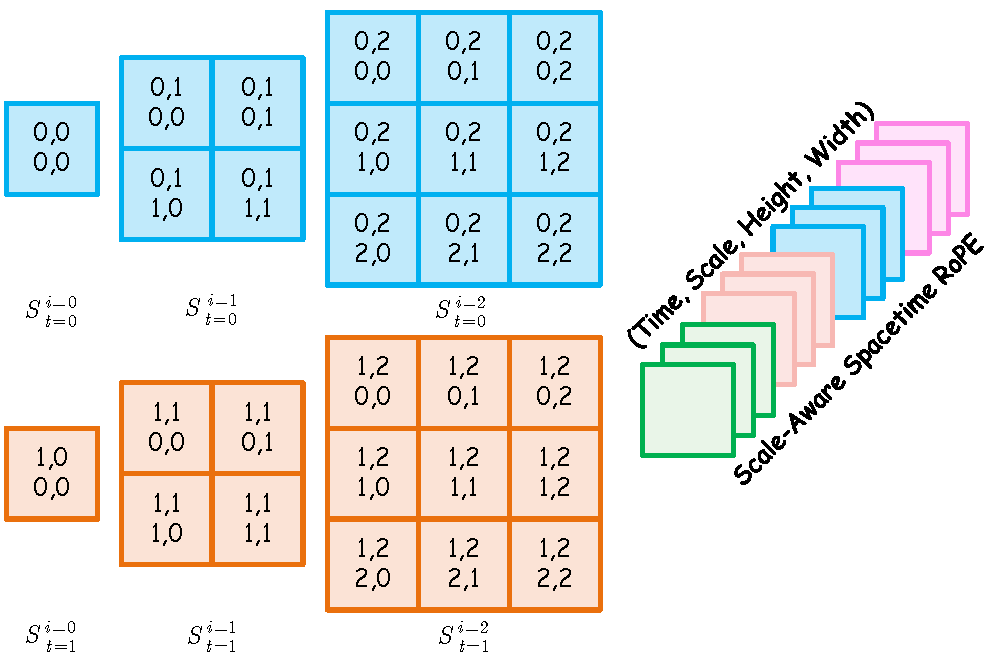
\includegraphics[width=0.95\linewidth]{fig/fig_SAROPE.pdf}
     \caption{\textbf{Scale-Aware spacetime RoPE (SA-RoPE).} To mitigate error accumulation in continuous latent spaces, SA-RoPE factorizes positional information into orthogonal rotational components across time, scale, and spatial dimensions. 
     }
    \label{fig:fig_SAROPE}
    \vspace{-1ex}
\end{figure}


\subsection{Long-horizon Spatiotemporal Consistency Enforcement}
\label{Sec3:Consistency}
Autoregressive models operating within continuous latent spaces are inherently susceptible to error accumulation~\cite{pasini2024continuous}. In this regime, minor deviations in early frames can rapidly propagate and cascade into severe structural degradation over extended horizons. In contrast to discrete representations, which implicitly rectify errors by quantizing latents to the nearest codebook centroid~\cite{van2017neural}, continuous errors can accumulate unboundedly. To mitigate this issue, we incorporate a strong structural inductive bias via SA-RoPE and an inference-time physical constraint known as Flow Rectification~\cite{liuflow}.

While standard RoPE~\cite{su2024roformer} effectively handles 1D sequences or 2D spatial grids, SAMPO++ operates on a more complex 4D manifold defined by coordinates $(t, s, h, w)$ representing time, scale, height, and width. Omitting the scale dimension in positional encoding introduces ambiguity, as the attention mechanism struggles to distinguish between structurally similar features originating from different resolution levels. To address this limitation, we formulate a Scale-Aware spacetime RoPE (SA-RoPE) that factorizes positional information into orthogonal rotational components (see Figure~\ref{fig:fig_SAROPE}). For a query vector $\boldsymbol{q}$ located at $(t, s, h, w)$, the transformed embedding is obtained via the composition of three independent rotations:
\begin{equation}
    \boldsymbol{q}' = \boldsymbol{q} \boldsymbol{R}_{\text{time}}(t) \boldsymbol{R}_{\text{scale}}(s) \boldsymbol{R}_{\text{spatial}}(h, w).
\end{equation}
The term $\boldsymbol{R}_{\text{scale}}(s)$ is critical for our scale-wise generation paradigm as it explicitly encodes the frequency level of the current feature. This enables attention heads to learn specialized behaviors, such as retrieving global structure from coarse scales ($s=1$) versus refining local textures at fine scales ($s=S$). By rigorously anchoring features within this 4D coordinate system, the model preserves superior structural coherence across long temporal windows.

\begin{algorithm}[t]
\caption{SAMPO++ Training (End-to-End)}
\label{algo:training}
\begin{algorithmic}[1]
\REQUIRE Dataset $\mathcal{D}$, Encoder $\mathcal{E}$, Causal Planner $\mathcal{T}$, FlowNet $v_\theta$, Downsample $\mathcal{P}_{\downarrow}$
\STATE $(\boldsymbol{x}, \boldsymbol{a}) \sim \mathcal{D}$; $\boldsymbol{z} = \mathcal{E}(\boldsymbol{x})$; Pyramid $\mathcal{Z} = \{\mathcal{P}_{\downarrow}(\boldsymbol{z}_t)\}_{t=1, s=1}^{T, S}$;
\STATE $\mathcal{L}_{\text{total}} = 0$;
\FOR{$t = 1, \dots, T$}
    \STATE $\hat{\boldsymbol{h}}_t = \mathcal{T}(\boldsymbol{z}_{<t}^S, \boldsymbol{a}_{<t})$; 
    \STATE $\boldsymbol{z}_t^0 = \boldsymbol{0}$; 
    \FOR{$s = 1, \dots, S$}
        \STATE $\tau \sim U(0,1), \ \boldsymbol{\epsilon} \sim \mathcal{N}(\boldsymbol{0}, \boldsymbol{I})$;
        \STATE $\boldsymbol{x}_\tau = (1-\tau)\boldsymbol{\epsilon} + \tau \boldsymbol{z}_t^s$; \ \ $\boldsymbol{c} = [ \text{up}(\boldsymbol{z}_t^{s-1}) , \hat{\boldsymbol{h}}_t ]$;
        \STATE $\boldsymbol{m} = \text{ADM}(\boldsymbol{a}_t, s)$; \ \ $\hat{\boldsymbol{v}} = v_\theta(\boldsymbol{x}_\tau, \tau, \boldsymbol{c}, \boldsymbol{m})$;
        \STATE $\mathcal{L}_{\text{Flow}} = \|\hat{\boldsymbol{v}} - (\boldsymbol{z}_t^s - \boldsymbol{\epsilon})\|_2^2$;
        \STATE $\mathcal{L}_{\text{total}} \leftarrow \mathcal{L}_{\text{total}} + w_s \cdot \mathcal{L}_{\text{Flow}}$;
    \ENDFOR
\ENDFOR
\STATE Update all parameters $(\theta_{\mathcal{T}}, \theta_{v})$ via $\nabla \mathcal{L}_{\text{total}}$;
\end{algorithmic}
\end{algorithm}
\begin{algorithm}[t]
\caption{SAMPO++ Inference}
\label{algo:inference}
\begin{algorithmic}[1]
\REQUIRE Context Frames $\boldsymbol{x}_{\text{ctx}}$, Action Plan $\boldsymbol{a}_{\text{fut}}$, Decoder $\mathcal{D}$
\STATE Initialize history buffer: $\mathcal{H} = \{ \mathcal{E}(\boldsymbol{x}_{\text{ctx}})^S \}$; 
\FOR{$k = 1, \dots, K$}
    \STATE $\hat{\boldsymbol{h}}_k = \mathcal{T}(\mathcal{H}, \boldsymbol{a}_{<k})$;
    \STATE $\boldsymbol{z}_k^0 = \boldsymbol{0}$; 
    \FOR{$s = 1, \dots, S$}
        \STATE $\boldsymbol{c} = [ \text{up}(\boldsymbol{z}_k^{s-1}), \hat{\boldsymbol{h}}_k ]$;
        \STATE $\boldsymbol{m} = \text{ADM}(\boldsymbol{a}_k, s)$; 
        \STATE $\boldsymbol{z}_k^s = \text{ODESolve}\big(\mathcal{N}(\boldsymbol{0}, \boldsymbol{I}), v_\theta(\cdot, \tau, \boldsymbol{c}, \boldsymbol{m}), \text{Rectify}\big)$; 
    \ENDFOR
    \STATE $\mathcal{H} \leftarrow \mathcal{H} \cup \{\boldsymbol{z}_k^S\}$; 
\ENDFOR
\RETURN $\hat{\boldsymbol{x}}_{\text{fut}} = \mathcal{D}(\mathcal{H}_{\text{fut}})$;
\end{algorithmic}
\end{algorithm}

Although SA-RoPE imparts structural awareness during the training phase, it does not actively mitigate latent drift during the inference process. To enforce strict physical consistency, we introduce a flow trajectory rectification strategy that operates as an energy-based guidance mechanism during sampling. We postulate that the temporal evolution of latent features must maintain consistency with the estimated optical flow. Let $\boldsymbol{F}_{t-1 \to t}$ denote the dense optical flow field predicted by a lightweight estimator, such as RAFT~\cite{teed2020raft}. We define a consistency energy function $E(\boldsymbol{z}_t^s)$ to measure the discrepancy between the generated latent and the warped state of the previous frame:
\begin{equation}
    E(\boldsymbol{z}_t^s) = \frac{1}{2} \| \boldsymbol{z}_t^s - \mathcal{W}(\boldsymbol{z}_{t-1}^s, \boldsymbol{F}_{t-1 \to t}) \|_2^2,
\end{equation}
where $\mathcal{W}$ denotes the warping operator. Given that Flow Matching generation entails solving the probability flow ODE~\cite{lipman2023flow, albergo2025stochastic}, we rectify the trajectory by augmenting the velocity field $v_\theta$ at each integration step. This is achieved by injecting the negative gradient of the consistency energy:
\begin{equation}
    v_{\text{rectified}}(\boldsymbol{z}_\tau, \tau) = v_\theta(\boldsymbol{z}_\tau, \tau) - \lambda(\tau) \nabla_{\boldsymbol{z}_\tau} E(\boldsymbol{z}_\tau),
\end{equation}
where $\lambda(\tau)$ is a time-dependent guidance scale. This operation effectively steers the generative trajectory towards physically plausible states that respect optical flow continuity equations, thereby significantly extending the stable rollout horizon without requiring retraining of the base model.

The complete training and inference procedures of SAMPO++ are summarized in Algorithm~\ref{algo:training} and Algorithm~\ref{algo:inference}, respectively. Notably, during the inference phase, we utilize the KV cache~\cite{pope2023efficiently} within the autoregressive causal planner to efficiently generate each temporal context $\boldsymbol{h}_t$ without redundant historical computation.
\section{Experiments and Analysis}
\label{Sec4:Experiments}


\subsection{Experimental Setup}

\textbf{Datasets.} 
To rigorously substantiate the efficacy and scalability of SAMPO++ as a foundational world model, we construct a comprehensive evaluation protocol spanning three distinct and highly challenging domains:
\textbf{(1) Robotic Manipulation.} Serving as our primary testbed for embodied physical interactions, we leverage the BAIR Robot Pushing dataset~\cite{ebert2017selfBAIR} to evaluate fundamental kinematic consistency. Characterized by its severe inherent stochasticity, this benchmark encompasses over 40K video sequences paired with end-effector actions, rigorously testing the model's capacity to handle uncertain environmental dynamics. To systematically assess cross-embodiment and cross-viewpoint generalization, we employ RoboNet~\cite{dasari2019robonet}, a massive-scale repository comprising 15M video frames aggregated from seven disparate robotic platforms. Furthermore, to push the limits of high-fidelity synthesis in visually complex scenarios, we incorporate the 1X World Model Dataset~\cite{1X_Technologies_1X_World_Model_2024}. Featuring long-horizon teleoperation of EVE humanoid androids in highly cluttered, unstructured environments, this dataset imposes a stringent stress test on fine-grained textural generation and long-term spatiotemporal coherence.
\textbf{(2) Embodied Control and Policy Learning.} Transcending passive video prediction, we rigorously evaluate the generative model's viability as a reactive, dynamic simulator for closed-loop action execution across two distinct paradigms. First, for Visual Planning, we utilize the $\text{VP}^2$ benchmark~\cite{tian2023control} to explicitly assess the model's capacity to serve as a forward dynamics oracle for Model Predictive Control (MPC) within the complex RoboDesk suite. Second, for Model-Based Reinforcement Learning (MBRL), we employ the Meta-World benchmark~\cite{yu2020meta} to evaluate performance across diverse manipulation skills. By quantifying the zero-shot transfer success rate of downstream agents—trained exclusively within the world model's synthesized latent environments and evaluated in the ground-truth physics simulator—we definitively verify the physical reliability and actionable utility of our generated dynamics.
\textbf{(3) Autonomous Driving.} To demonstrate the paradigm's scalability to highly dynamic, ego-centric outdoor environments, we extend our evaluation to the autonomous driving domain utilizing Cityscapes~\cite{Cityscapes} and a curated subset of OpenDV-YouTube~\cite{yang2024genad}. In stark contrast to static robotic setups, these datasets introduce severe visual challenges such as high-speed ego-motion, complex lighting variations, and unpredictable multi-agent traffic dynamics. Evaluated primarily under an action-free future prediction setting, this domain isolates and validates SAMPO++'s capacity for open-world visual dynamics modeling, underscoring its potential as a robust foundational prior for next-generation neural driving simulators.

\textbf{Baselines.} We benchmark SAMPO++ against a representative set of state-of-the-art architectures that span the two dominant paradigms in generative world modeling. Within the discrete autoregressive regime, we compare against iVideoGPT~\cite{wu2024ivideogpt} and our conference predecessor, SAMPO~\cite{wang2025sampo}. This axis of comparison explicitly isolates the architectural gains achieved by supplanting discrete vector quantization with our continuous scale-wise flow matching formulation. Conversely, within the continuous generative regime, we evaluate against SyncVP~\cite{Pallotta_2025_CVPR} and STDiff~\cite{STDiff} as strong baselines. SyncVP represents recent advancements in multi-modal synchronous prediction, whereas STDiff leverages stochastic differential equations (SDEs) for continuous temporal modeling, thereby providing a robust comparative foundation for evaluating our ODE-based optimal transport trajectories.

\textbf{Metrics.} Our evaluation protocol assesses the world model across three complementary perspectives. First, for Visual Fidelity, we report Fréchet Video Distance (FVD)~\cite{FVDunterthiner2018towards} as the primary metric for temporal coherence, complemented by PSNR~\cite{PSNRhuynh2008scope}, SSIM~\cite{SSIMwang2004image}, and LPIPS~\cite{LPIPSzhang2018unreasonable} for perceptual frame quality. Second, for Visual Planning, we evaluate the model's capacity to serve as a forward dynamics oracle for Model Predictive Control (MPC) and report the task success rate on manipulation tasks. Third, for Model-Based Reinforcement Learning (MBRL), we train agents entirely inside the imagined world and evaluate their zero-shot transfer success rate and average reward in the ground-truth physics simulator.


\textbf{Implementation Details.} 
(1) Continuous Multi-Scale Tokenizer.
We employ the VA-VAE~\cite{yao2025reconstruction} architecture to serve as our asymmetric continuous tokenizer. To ensure robust spatial representation and cross-domain feature extraction, our tokenizer is comprehensively pre-trained on both the Open X-Embodiment~\cite{o2024open} and Cityscapes~\cite{Cityscapes} using a combination of reconstruction and commitment losses.
(2) Decoupled Continuous-Flow Transformer.
We employ a decoupled two-stage architecture for temporal dynamics and visual synthesis. An autoregressive decoder-only backbone models macroscopic semantic transitions~\cite{wang2025sampo}, while a LightningDiT-based network~\cite{yao2025reconstruction}, equipped with RMSNorm and SwiGLU activations, renders these representations into fine-grained visual details via flow matching. To facilitate continuous autoregressive training, a learnable start embedding is prepended to each sequence, allowing the model to unroll future states conditioned on ground-truth history. Following~\cite{wang2025sampo}, our backbones are pre-trained on Open X-Embodiment~\cite{o2024open} and Cityscapes~\cite{Cityscapes}.
(3) Optimization and Training Setup.
The training pipeline is unified across all environments and resolutions, executed on 8 NVIDIA A800 GPUs. Both the autoregressive temporal planner and the scale-wise flow network are optimized using the AdamW optimizer with a base learning rate of $1 \times 10^{-4}$ and momentum parameters $\beta_1=0.9$ and $\beta_2=0.999$. To stabilize the early training dynamics of the deep continuous vector fields, we apply a cosine learning rate scheduler with a linear warmup period of 5,000 steps. Weight decay is uniformly set to $0.01$ across the Transformer backbones to prevent overfitting while preserving representation capacity. 
Furthermore, all models are trained in \texttt{bfloat16} mixed precision to significantly accelerate computation and reduce memory footprints.


\subsection{High-Fidelity Video Prediction}
\begin{table*}[t]
\caption{\textbf{Video prediction results on BAIR and RoboNet datasets.} Following standard evaluation protocols, models are tasked with predicting 15 future frames conditioned on a single context frame for the BAIR ($1 \rightarrow 15$ frames), and 10 future frames conditioned on two context frames for the RoboNet ($2 \rightarrow 10$ frames). We evaluate the generation fidelity on both datasets across 3 random seeds and report the mean and standard deviation. ``-'' indicates values not reported in the original papers. Note that LPIPS and SSIM are scaled by 100 for better readability. 
}
\label{tab:video_pred}
\centering
\scalebox{1.1}{ 
    \begin{tabular}{lcccc|lcccc}
        \toprule
        \textbf{BAIR}~\cite{ebert2017selfBAIR}     & \multicolumn{1}{l}{FVD↓} & \multicolumn{1}{l}{PSNR↑} & \multicolumn{1}{l}{SSIM↑} & \multicolumn{1}{l|}{LPIPS↓} & \textbf{RoboNet}~\cite{dasari2019robonet}   & \multicolumn{1}{l}{FVD↓} & \multicolumn{1}{l}{PSNR↑} & \multicolumn{1}{l}{SSIM↑} & \multicolumn{1}{l}{LPIPS↓} \\ \midrule
        \rowcolor{grey}
        \multicolumn{5}{c|}{\textit{action-free \& 64×64 resolution}}                                                           & \multicolumn{5}{c}{\textit{action-conditioned \& 64×64 resolution}}                                                   \\
        MaskViT~\cite{gupta2022maskvit}   & 93.7                    & -                        & -                        & -                          & MaskViT~\cite{gupta2022maskvit}   & 133.5                   & 23.2                     & 80.5                     & 4.2                       \\
        FitVid~\cite{babaeizadeh2021fitvid}    & 93.6                    & -                        & -                        & -                          & FitVid~\cite{babaeizadeh2021fitvid}    & 62.5                    & 28.2                     & 89.3                     &\textbf{2.4}                       \\
        MCVD~\cite{voleti2022mcvd}      & 89.5                    & 16.9                     & 78.0                     & -                          & SVG~\cite{villegas2019high}       & 123.2                   & 23.9                     & 87.8                     & 6.0                       \\
        MAGVIT~\cite{yu2023magvit}    & 62.0                    & 19.3                     & 78.7                     & 12.3                       & GHVAE~\cite{wu2021greedy}     & 95.2                    & 24.7                     & 89.1                     & 3.6                       \\
        iVideoGPT~\cite{wu2024ivideogpt} & 75.0                    & 20.4                     & 82.3                     & 9.5                        & iVideoGPT~\cite{wu2024ivideogpt} & 63.2                    & 27.8                     & 90.6                     & 4.9                       \\ 
        SAMPO~\cite{wang2025sampo} & 65.7 & 22.3 & 86.7 & 8.4 & SAMPO~\cite{wang2025sampo} & 57.1 & 29.3 & 94.1 & 3.3 \\
        \midrule
        \rowcolor{lightblue}
        SAMPO++ (Ours) & \textbf{59.4}$^{\pm 1.5}$ & \textbf{23.1}$^{\pm 0.2}$ & \textbf{88.5}$^{\pm 0.4}$ & \textbf{7.2}$^{\pm 0.1}$ & SAMPO++ (Ours) & \textbf{49.8}$^{\pm 1.2}$ & \textbf{30.5}$^{\pm 0.1}$ & \textbf{95.2}$^{\pm 0.2}$ & 2.6$^{\pm 0.1}$ \\

        \midrule
        \rowcolor{grey}
        \multicolumn{5}{c|}{\textit{action-conditioned \& 64×64 resolution}}                                                    & \multicolumn{5}{c}{\textit{action-conditioned \& 256×256 resolution}}                                                 \\
        MaskViT~\cite{gupta2022maskvit}   & 70.5                    & -                        & -                        & -                          & MaskViT~\cite{gupta2022maskvit}   & 211.7                   & 20.4                     & 67.1                     & 17.0                      \\
        iVideoGPT~\cite{wu2024ivideogpt} & 60.8                    & 24.5                     & 90.2                     & 5.0                        & iVideoGPT~\cite{wu2024ivideogpt} & 197.9                   & 23.8                     & 80.8                     & 14.7                      \\
        SAMPO~\cite{wang2025sampo}     & \multicolumn{1}{c}{55.5}    & \multicolumn{1}{c}{26.7}     & \multicolumn{1}{c}{94.7}     & \multicolumn{1}{c|}{3.7}      & SAMPO-L~\cite{wang2025sampo}    & \multicolumn{1}{c}{175.3}    & \multicolumn{1}{c}{25.3}     & \multicolumn{1}{c}{84.7}     & \multicolumn{1}{c}{12.3}      \\ 
    
        \midrule
        \rowcolor{lightblue}
        SAMPO++ (Ours) & \textbf{47.6}$^{\pm 1.8}$ & \textbf{27.9}$^{\pm 0.3}$ & \textbf{96.1}$^{\pm 0.3}$ & \textbf{3.1}$^{\pm 0.1}$ & SAMPO++ (Ours) & \textbf{152.4}$^{\pm 3.5}$ & \textbf{26.8}$^{\pm 0.2}$ & \textbf{87.5}$^{\pm 0.5}$ & \textbf{9.8}$^{\pm 0.3}$ \\
    
        \bottomrule
    \vspace{-3ex}
    \end{tabular}
}
\end{table*}
\textbf{Short-term Prediction.}
We first evaluate short-term video prediction capabilities across diverse robotic datasets. Quantitative results on the BAIR and RoboNet benchmarks are summarized in Table~\ref{tab:video_pred}, while performance on the visually complex 1X World Model dataset is detailed in Table~\ref{tab:1X}.
\begin{table}[t]
\centering
\caption{\textbf{Video prediction results on the 1X dataset.} We predict 10 future frames from 2 context frames.}
\label{tab:1X}

\scalebox{1.1}{
\begin{tabular}{lcccc}
\toprule
\textbf{1X WM}~\cite{1X_Technologies_1X_World_Model_2024} & FVD$\downarrow$ & PSNR$\uparrow$ & SSIM$\uparrow$ & LPIPS$\downarrow$ \\
\midrule
\rowcolor{gray!20} \multicolumn{5}{c}{\textit{Action-Conditioned ($256\times256$)}} \\
iVideoGPT~\cite{wu2024ivideogpt} & 251.8 & 24.1 & 78.3 & 20.3 \\
SAMPO~\cite{wang2025sampo}       & 227.1 & 25.7 & 80.3 & 18.7 \\
\midrule
\rowcolor{blue!10} SAMPO++ (Ours) & \textbf{188.5} & \textbf{26.8} & \textbf{83.1} & \textbf{16.4} \\
\bottomrule
\vspace{-4ex}
\end{tabular}
}
\end{table} 

As evidenced in Table~\ref{tab:video_pred}, SAMPO++ achieves state-of-the-art performance across all metrics. Specifically, on the RoboNet dataset ($256 \times 256$), SAMPO++ yields an FVD of \textbf{152.4}, significantly outperforming the discrete baseline SAMPO (175.3) and iVideoGPT (197.9). We attribute this substantial performance leap to our fundamental paradigm shift from a discrete codebook to a continuous latent manifold. Discrete autoregressive models inevitably suffer from quantization noise, which manifests as high-frequency flickering and loss of fine textures in the generated video. By employing scale-wise flow matching, SAMPO++ effectively models the continuous probability density of visual features, thereby recovering intricate spatial details lost by vector quantization.
On the 1X World Model dataset—which features complex humanoid manipulations in cluttered environments and serves as a rigorous stress test for fine-grained generation—SAMPO++ achieves an FVD of \textbf{198.5} and an LPIPS of \textbf{16.4}, substantially surpassing iVideoGPT (FVD 251.8). While discrete tokens struggle to encode the subtle finger movements of the EVE robot, our continuous approach, enhanced by Action-adaptive Dynamics Modulation (ADM), precisely captures these micro-dynamics, resulting in sharper and physically more plausible motion.


\textbf{Long-term Generation.}
\begin{table}[t]
\centering
\caption{\textcolor{blue}{\textbf{Long-term video prediction on BAIR datasets.} We report results under two rigorous settings: standard long-horizon prediction ($2 \rightarrow 28$ frames) and extended long-horizon prediction ($2 \rightarrow 48$ frames). The results of SyncVP for 48 frames are reproduced using their official checkpoints. $\#$T denotes the number of sampled trajectories used for evaluation.
$\dagger$: Model utilizes depth information for multi-modal prediction.}}
\label{tab:bairbenchmark}
\scalebox{1.2}{ 
    \begin{tabular}{lcccc}
    \toprule
    \textbf{BAIR}~\cite{ebert2017selfBAIR} & \#T & FVD $\downarrow$ & SSIM $\uparrow$ & LPIPS $\downarrow$ \\
    \midrule
    \rowcolor{gray!20} \multicolumn{5}{c}{\textit{Standard Prediction: 2 $\rightarrow$ 28 frames}} \\
    NPVP~\cite{ye2023unified}            & 100 & 923.6 & 84.2 & 5.7 \\
    STM-FANet~\cite{stmfanet}            & -   & 159.6 & 84.4 & 9.4 \\
    VPTR-NAR~\cite{ye2022vptr}           & -   & -     & 81.3 & 7.0 \\
    Hier-VRNN~\cite{Castrejon_2019_ICCV}& 100 & 143.4 & 82.9 & 5.5 \\
    MCVD~\cite{MCVD}                     & 10  & 120.6 & 78.5 & 7.1 \\
    SAVP~\cite{lee2018savp}              & 100 & 116.4 & 78.9 & 6.3 \\
    ExtDM-K4~\cite{ExtDM}                & 100 & 102.8 & 81.4 & 6.9 \\
    STDiff~\cite{STDiff}                 & 10  & 88.1  & 81.8 & 6.9 \\
    SyncVP~\cite{Pallotta_2025_CVPR}     & 10  & 70.5  & 79.5 & 7.9 \\
    SyncVP$^{\dagger}$                   & 10  & 63.6  & 80.5 & 7.5 \\
    SAMPO~\cite{wang2025sampo}           & 10   & 65.7  & 86.7 & 5.9 \\
    \midrule
    \rowcolor{blue!10} SAMPO++ (Ours)    & 10   & \textbf{52.5} & \textbf{88.5} & \textbf{4.6} \\
    
    \midrule
    \rowcolor{gray!20} \multicolumn{5}{c}{\textit{Long-Horizon Prediction: 2 $\rightarrow$ 48 frames}} \\
    SyncVP~\cite{Pallotta_2025_CVPR}     & 10  & 105.3 & 72.4 & 8.8 \\
    SyncVP$^{\dagger}$                   & 10  & 92.1  & 74.8 & 8.4 \\
    SAMPO~\cite{wang2025sampo}           & 10   & 81.3  & 83.2 & 6.7 \\
    \midrule
    \rowcolor{blue!10} SAMPO++ (Ours)    & 10   & \textbf{64.8} & \textbf{86.1} & \textbf{5.4} \\
    \bottomrule
    \vspace{-4ex}
    \end{tabular}
}
\end{table}
Sustained spatiotemporal consistency over extended horizons is a critical requirement for a robust world model. However, conventional autoregressive and diffusion-based paradigms are inherently susceptible to rapid structural degradation during prolonged temporal rollouts. As evidenced in Table~\ref{tab:bairbenchmark}, the strong diffusion baseline, SyncVP, experiences significant performance degradation, with its FVD deteriorating from 70.49 ($T=28$) to 105.32 ($T=48$). This vulnerability fundamentally stems from the stochastic nature of iterative diffusion sampling, which compounds microscopic structural errors—frequently manifesting as visual hallucinations—across recursive generation steps.
In contrast, SAMPO++ exhibits exceptional predictive stability, sustaining a low FVD of \textbf{64.8} even at 48 frames. This sustained fidelity rigorously corroborates the efficacy of our proposed flow trajectory rectification strategy and Scale-Aware spacetime RoPE. Specifically, the rectification mechanism actively constrains the continuous latent trajectory within the physically plausible manifold during inference, effectively circumventing the unbounded latent drift endemic to naive autoregressive or diffusion approaches. Most notably, the long-term predictive performance of SAMPO++ (FVD 64.8) surpasses even the short-term performance of the prior discrete state-of-the-art, SAMPO (FVD 65.7). This result decisively demonstrates that our unified continuous-flow paradigm fundamentally mitigates the pervasive challenge of long-horizon structural degradation.

\subsection{Generalization to Autonomous Driving}
\begin{table}[t]
\centering
\caption{\textcolor{blue}{\textbf{Lone-term video prediction on Cityscapes dataset.} We report results under two rigorous horizons: standard prediction ($2 \rightarrow 28$ frames) and extended long-horizon prediction ($2 \rightarrow 48$ frames). The $\dagger$ symbol indicates baseline results rigorously reproduced locally utilizing the authors' official pre-trained checkpoints. The best and second-best results are highlighted in \textbf{bold} and \underline{underline}, respectively.}}
\label{tab:video_AD}

\scalebox{1.15}{
\begin{tabular}{lcccc}
    \toprule
    \textbf{Cityscapes}~\cite{Cityscapes} & \#T & FVD $\downarrow$ & SSIM $\uparrow$ & LPIPS $\downarrow$ \\
    \midrule
    \rowcolor{gray!20} \multicolumn{5}{c}{\textit{Standard Prediction: Cityscapes, 2 $\rightarrow$ 28 frames}} \\
    SVG-LP~\cite{svg-lp}                & 100 & 1300.26 & 0.574 & 549.0 \\
    NPVP~\cite{ye2023unified}           & 100 & 768.04  & 0.744 & 183.2 \\
    VRNN 1L~\cite{Castrejon_2019_ICCV}  & 100 & 682.08  & 0.609 & 304.0 \\
    Hier-VRNN~\cite{Castrejon_2019_ICCV}& 100 & 567.51  & 0.628 & 264.0 \\
    GHVAEs~\cite{ghvaes}                & -   & 418.00  & 0.740 & 194.0 \\
    VDT~\cite{VDT}                      & -   & 142.3   & \textbf{0.880} & - \\
    MCVD~\cite{MCVD}                    & 10  & 141.31  & 0.690 & 112.0 \\
    ExtDM-K4~\cite{ExtDM}               & 100 & 121.3   & 0.745 & 108.0 \\
    STDiff~\cite{STDiff}                & 10  & 107.31  & 0.658 & 136.2 \\
    SyncVP~\cite{Pallotta_2025_CVPR}    & 10  & 97.31   & 0.652 & 161.1 \\
    SyncVP$^{\dagger}$~\cite{Pallotta_2025_CVPR} & 10 & 84.00 & 0.649 & 159.7 \\
    SAMPO~\cite{wang2025sampo}          & 10  & 92.50   & 0.765 & 124.5 \\ 
    \midrule
    \rowcolor{blue!10} SAMPO++ (Ours)   & 10  & \textbf{73.45} & \underline{0.788} & \textbf{94.5} \\ 
    
    \midrule
    \rowcolor{gray!20} \multicolumn{5}{c}{\textit{Long-Horizon Prediction: Cityscapes, 2 $\rightarrow$ 48 frames}} \\
    SyncVP~\cite{STDiff}                & 10  & 184.20  & 0.542 & 188.4 \\
    SyncVP$^{\dagger}$     & 10  & 165.80  & 0.565 & 192.1 \\
    SAMPO~\cite{wang2025sampo}          & 10  & 145.60  & 0.680 & 156.0 \\
    \midrule
    \rowcolor{blue!10} SAMPO++ (Ours)   & 10  & \textbf{118.42} & \textbf{0.715} & \textbf{135.2} \\
    \bottomrule
    \vspace{-4ex}
    \end{tabular}
    }
\end{table}


To systematically demonstrate that SAMPO++ transcends robotic manipulation to function as a general-purpose neural world simulator, we extend our evaluation to the Cityscapes dataset. This domain inherently introduces severe challenges, including high-speed ego-motion and complex multi-agent traffic dynamics. Quantitative results are detailed in Table~\ref{tab:video_AD}.

A notable observation from Table~\ref{tab:video_AD} is that SAMPO++ (FVD \textbf{73.45}) consistently outperforms the strong continuous baseline, SyncVP$^{\dagger}$ (FVD 84.00). Notably, while SyncVP$^{\dagger}$ relies on auxiliary ground-truth depth maps during training to guide its geometric learning, SAMPO++ operates exclusively on raw RGB video streams. This superiority strongly suggests that our ``Predict-then-Refine'' paradigm implicitly acquires robust 3D geometric awareness and scene depth estimation derived entirely from scale-wise structural priors, thereby circumventing the need for explicit geometric supervision.


% \begin{table}[t]
    \centering
    \resizebox{\linewidth}{!}{%
    \begin{tabular}{lccc} %
        \toprule
        \textbf{OpenDV-YouTube} & \multicolumn{3}{c}{256x256 resolution, 2 $\rightarrow$ 14} \\ % 
        \cmidrule(lr){2-4}
        Model & FVD$\downarrow$ & SSIM$\uparrow$ & LPIPS$\downarrow$ \\ % 
        \midrule
        SyncVP~\cite{Pallotta_2025_CVPR} & 238.7 & 0.653 & 247.1 \\ SyncVP$^{\dagger}$~\cite{Pallotta_2025_CVPR} & 225.4 & 0.675 & 230.5 \\ 
        Open-Sora~\cite{opensora} & 184.7 & 0.693 & 210.2 \\ 
        \midrule 
        \rowcolor{lightblue}TriFlow-S & 198.6 & 0.737 & 195.4 
        \bottomrule
    \end{tabular}
    }
    \caption{\textbf{Quantitative results on OpenDV-YouTube.} 
    We evaluate generation fidelity at a higher spatial resolution.
    For a fair comparison, we retrained Open-Sora with its parameter count adjusted to match TriFlow-B model (detailed in Appendix~\ref{A:Architecture}). TriFlow demonstrates robust scalability across varying model capacities.
    % We evaluate generation fidelity at a higher spatial resolution. TriFlow demonstrates robust scalability across varying model capacities. 
    }
    \label{tab:opendv}
    \vspace{-4ex}
\end{table}
Autonomous driving scenarios are characterized by massive pixel displacements and rapid viewpoint transformations, which historically confound both pixel-level autoregressive architectures (\textit{e.g.}, MCVD, FVD 141.31) and standard diffusion models. SAMPO++ effectively navigates these topological challenges by hierarchically decoupling motion synthesis into macroscopic structural evolution (governed by the Temporal Planner) and microscopic textural integration (parameterized by Flow Matching). This rigorous scale-wise decoupling enables the model to preserve the structural integrity of high-frequency elements (\textit{e.g.}, poles, traffic signs) even under aggressive ego-motion, ultimately achieving highly competitive structural similarity (SSIM \underline{0.788}) among generative baselines.

Furthermore, under the highly demanding long-horizon setting ($2 \rightarrow 48$ frames), SAMPO++ significantly surpasses the reproduced SyncVP$^{\dagger}$ (FVD 118.42 vs. 165.80). This sustained spatiotemporal fidelity strongly validates SAMPO++'s potential as a robust forward dynamics engine for autonomous driving planning and closed-loop simulation.

\subsection{Embodied Control \& Policy Learning.}
\begin{table*}[t]
\small
\caption{\textbf{Quantitative evaluation of visual planning efficacy on the control-centric VP\(^2\) benchmark.} We report the downstream Task Success Rate (\%) across eight distinct robotic manipulation tasks. Following standard protocol~\cite{wang2025sampo,wu2024ivideogpt}, the aggregated average performance (\textit{Avg. Success}) explicitly excludes the ``Flat Block'' task due to its inherently low simulator upper bound. All metrics represent the mean and standard deviation computed across 3 independent random seeds.
}
\label{tab:vp2}
    \centering
    \resizebox{1.0\linewidth}{!}{
    \setlength{\tabcolsep}{0.5em}%
    \begin{tabular}{lcccccccc|c}
        \toprule
        \rowcolor{grey} \multicolumn{1}{l}{Method / Task} & \begin{tabular}[c]{@{}c@{}}Robosuite \\ Push\end{tabular} & \begin{tabular}[c]{@{}c@{}}Flat \\ Block\end{tabular} & \begin{tabular}[c]{@{}c@{}}Open\\ Drawer\end{tabular} & \begin{tabular}[c]{@{}c@{}}Open\\ Slide\end{tabular} & \begin{tabular}[c]{@{}c@{}}Blue\\ Button\end{tabular} & \begin{tabular}[c]{@{}c@{}}Green\\ Button\end{tabular} & \begin{tabular}[c]{@{}c@{}}Red\\ Button\end{tabular} & \begin{tabular}[c]{@{}c@{}}Upright\\ Block\end{tabular} & \begin{tabular}[c]{@{}c@{}}Avg.\\Success$\uparrow$\end{tabular}  \\
         \midrule
        Simulator & 93.5$^{\pm 1.2}$ & 13.3$^{\pm 0.0}$ & 76.7$^{\pm 0.0}$ & 71.7$^{\pm 1.4}$ & 100.0$^{\pm 0.0}$ & 96.7$^{\pm 0.0}$ & 90.0$^{\pm 0.0}$ & 90.0$^{\pm 0.0}$ & 100.0 \\
        \midrule
        FitVid~\cite{babaeizadeh2021fitvid} & 67.7$^{\pm 6.4}$ & \textbf{9.2$^{\pm 2.8}$} & 25.3$^{\pm 8.2}$ & \underline{35.3}$^{\pm 5.5}$ & 94.0$^{\pm 4.2}$ & 84.0$^{\pm 5.5}$ & 58.7$^{\pm 5.5}$ & 51.3$^{\pm 2.9}$ & 65.6 \\
        SVG'~\cite{villegas2019high} & 79.8$^{\pm 3.3}$  & 2.0$^{\pm 1.4}$ & 16.7$^{\pm 8.2}$ & \textbf{57.3}$^{\pm 11.0}$ & 97.3$^{\pm 2.7}$ & 81.3$^{\pm 5.5}$ & 76.0$^{\pm 9.5}$ & \underline{48.7}$^{\pm 11.1}$ & \underline{72.5} \\
        MCVD~\cite{voleti2022mcvd} & 77.3$^{\pm 2.1}$ & 4.0$^{\pm 1.4}$ & 11.7$^{\pm 1.4}$ & 18.3$^{\pm 1.4}$ & 95.0$^{\pm 4.1}$ & 83.3$^{\pm 0.0}$ & 73.3$^{\pm 2.7}$ & 56.7$^{\pm 2.7}$ & 64.3 \\
        MaskViT~\cite{gupta2022maskvit} & 82.6$^{\pm 2.5}$ & 4.0$^{\pm 4.1}$ & 4.0$^{\pm 4.1}$ & 8.7$^{\pm 5.5}$ & 94.7$^{\pm 1.4}$ & 64.0$^{\pm 4.1}$ & 24.0$^{\pm 8.2}$ & 62.2$^{\pm 9.5}$ & 52.1 \\
        Struct-VRNN~\cite{minderer2019unsupervised} & 55.4$^{\pm 4.1}$ & 4.7$^{\pm 5.5}$ & 2.7$^{\pm 4.2}$ & 12.7$^{\pm 6.9}$ & 86.7$^{\pm 4.2}$ & 68.0$^{\pm 9.5}$ & 30.7$^{\pm 4.2}$ & 33.3$^{\pm 2.7}$ & 44.2 \\
        iVideoGPT~\cite{wu2024ivideogpt} & 78.3$^{\pm 0.8}$ & 3.3$^{\pm 0.7}$ & 37.5$^{\pm 1.7}$ & 16.1$^{\pm 2.7}$ & 95.6$^{\pm 2.1}$ & 82.5$^{\pm 3.4}$ & 92.2$^{\pm 1.4}$ & 44.7$^{\pm 1.7}$ & 70.1 \\
        
        SAMPO~\cite{wang2025sampo} & \multicolumn{1}{c}{\underline{80.7}$^{\pm 1.4}$} & \multicolumn{1}{c}{5.5$^{\pm 1.2}$} & \multicolumn{1}{c}{\underline{40.3}$^{\pm 2.3}$} & \multicolumn{1}{c}{18.3$^{\pm 3.3}$} & \multicolumn{1}{c}{\underline{97.3}$^{\pm 1.7}$} & \multicolumn{1}{c}{\underline{85.3}$^{\pm 3.3}$} & \multicolumn{1}{c}{\underline{94.7}$^{\pm 2.1}$} & \multicolumn{1}{c|}{46.1$^{\pm 2.7}$} & \multicolumn{1}{c}{72.2} \\ 
        \midrule
        \rowcolor{blue!10} SAMPO++ (Ours) & \multicolumn{1}{c}{\textbf{86.2}$^{\pm 1.1}$} & \multicolumn{1}{c}{\underline{6.8}$^{\pm 0.9}$} & \multicolumn{1}{c}{\textbf{48.5}$^{\pm 1.5}$} & \multicolumn{1}{c}{32.4$^{\pm 2.1}$} & \multicolumn{1}{c}{\textbf{98.5}$^{\pm 0.5}$} & \multicolumn{1}{c}{\textbf{91.5}$^{\pm 1.2}$} & \multicolumn{1}{c}{\textbf{96.0}$^{\pm 1.1}$} & \multicolumn{1}{c|}{\textbf{64.5}$^{\pm 2.4}$} & \multicolumn{1}{c}{\textbf{75.4}} \\ \bottomrule

    \end{tabular}
    }
    \vspace{-3ex}
\end{table*}
\textbf{Visual Planning with Action-Conditioned Rollouts.}
To rigorously validate SAMPO++'s utility as a robust forward dynamics engine for closed-loop control, we employ the $\text{VP}^2$ benchmark~\cite{tian2023control}. Specifically, we evaluate the model on the RoboDesk suite~\cite{kannan2021robodesk}, a control-centric benchmark comprising complex, multi-stage manipulation tasks. Following standard evaluation protocols, the world models are trained on 35k noisy, scripted interaction trajectories. During the inference phase, we deploy a sampling-based Model Predictive Control (MPC) planner. This planner leverages the learned world model to simulate future visual trajectories conditioned on various candidate action sequences, ultimately executing the sequence that maximizes the predicted task reward. 

The quantitative success rates across eight distinct RoboDesk manipulation tasks are summarized in Table~\ref{tab:vp2}. SAMPO++ establishes a new state-of-the-art with an aggregate success rate of \textbf{75.4\%}, significantly outperforming the recent transformer-based baseline iVideoGPT (70.1\%) and our discrete predecessor SAMPO (72.2\%). 

A granular analysis of the task-specific performance reveals that our architectural advantage is most pronounced in kinematically dense tasks governed by continuous contact and friction, such as ``Open Slide'' and ``Open Drawer''. For instance, in the ``Open Slide'' task, SAMPO++ elevates the success rate from a mere 18.3\% (SAMPO) to \textbf{32.4\%}. This substantial performance delta exposes a fundamental limitation of discrete autoregressive models: the non-differentiable quantization of latent tokens induces ``jumpy'' or discretized dynamics. Subtle, continuous spatial displacements (\textit{e.g.}, sliding) are frequently snapped to the nearest codebook centroid, yielding physically inconsistent trajectories that ultimately misguide the MPC planner. By contrast, SAMPO++'s continuous flow matching formulation parameterizes smooth velocity fields, enabling the precise integration of friction-induced micro-motions.

Furthermore, in spatially targeted tasks such as the ``Red Button'' actuations, SAMPO++ consistently achieves near-perfect success rates ($>91\%$). This robust performance empirically corroborates the efficacy of our proposed Action-adaptive Dynamics Modulation (ADM). By actively injecting control signals directly into the normalization layers of the continuous flow network, ADM ensures that the generative dynamics remain strictly anchored to fine-grained action commands (\textit{e.g.}, targeted button pressing). This scale-aware structural conditioning effectively mitigates the ``control drift'' commonly observed in passive-conditioning baselines like FitVid~\cite{babaeizadeh2021fitvid}, thereby yielding a reliable visual simulator for interactive planning.


\begin{figure*}[ht]
    \centering
    \begin{minipage}{0.3\linewidth}
        \centering
        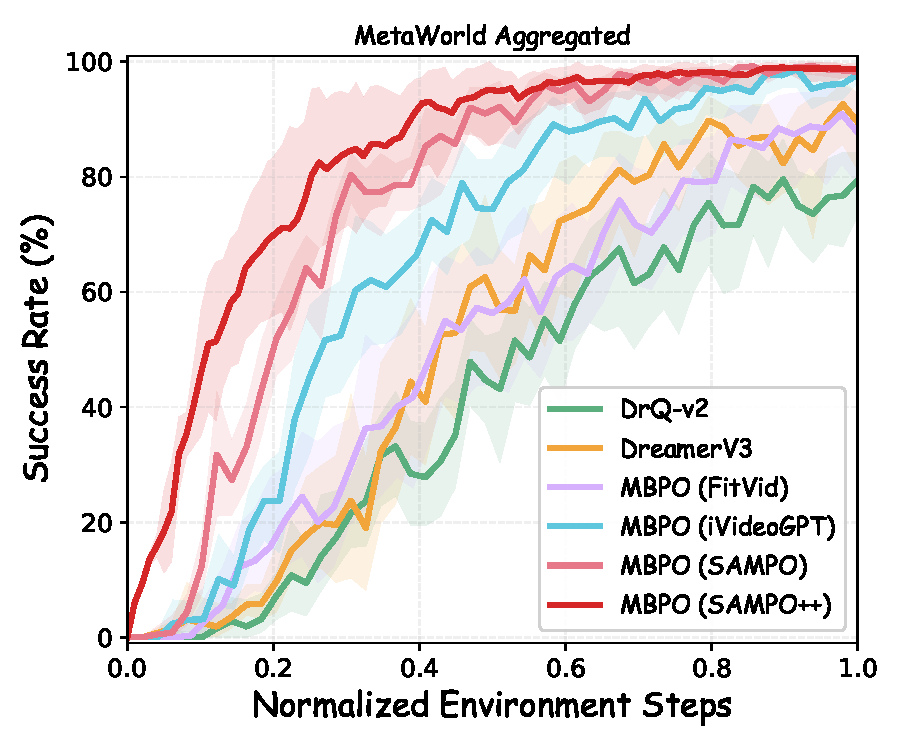
\includegraphics[width=\linewidth]{fig/metaworld_aggregate.pdf}
    \end{minipage}
    \begin{minipage}{0.65\linewidth}
        \centering
        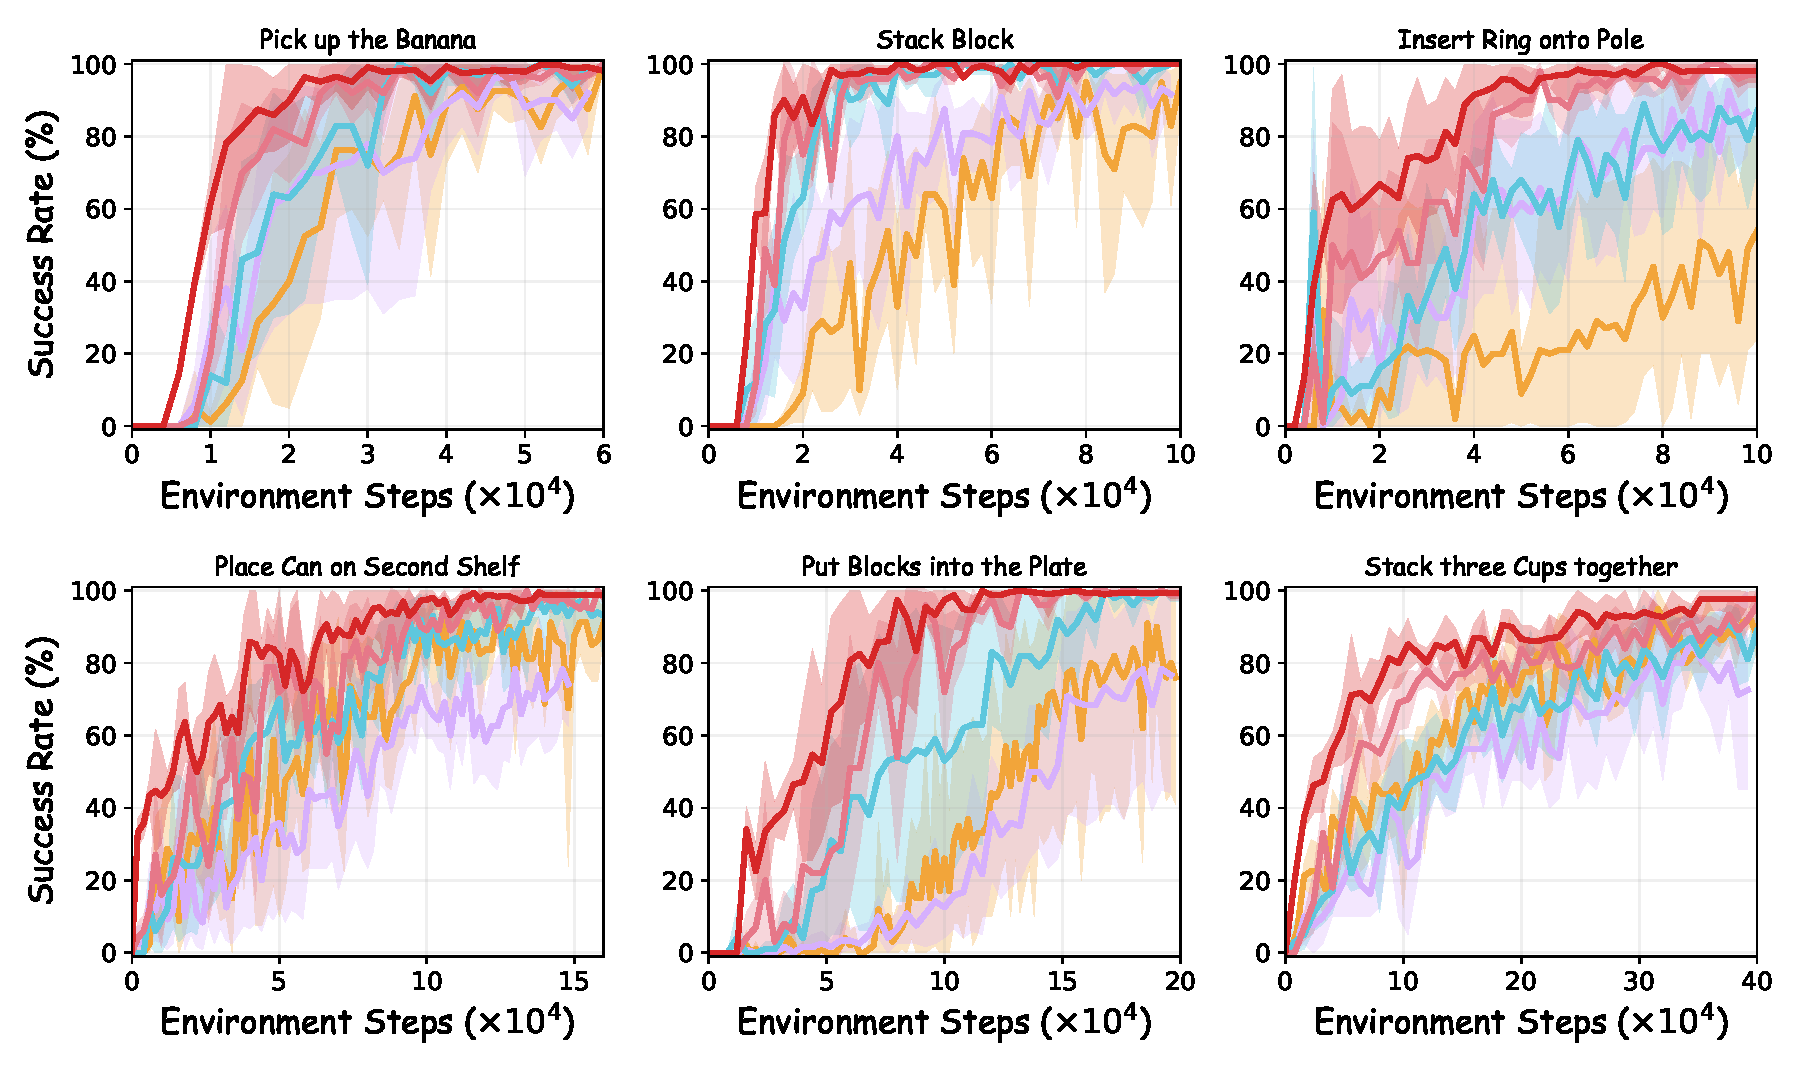
\includegraphics[width=\linewidth]{fig/metaworld_single.pdf}
    \end{minipage}\hspace{0.01\linewidth}
    \caption{\textbf{Model-based RL on Meta-world with SAMPO++.} \textbf{(Left)} Aggregated performance report the Interquartile Mean (IQM) and 95\% confidence intervals (CI) over 30 runs (5 seeds $\times$ 6 tasks). \textbf{(Right)} Task-specific learning curves showing the mean success rate (\%) and 95\% CI across 5 random seeds. Success rates are evaluated over 20 independent episodes per training checkpoint. All generative baselines act as pre-trained world models~\cite{seo2022reinforcement}.
    }% , supplying synthetic interactive rollouts for downstream policy optimization.}
    \label{fig:RL}
    \vspace{-2ex}
\end{figure*}

\textbf{Model-Based Reinforcement Learning Utility.}
Moving beyond open-loop planning, we rigorously assess SAMPO++'s capacity to serve as a dynamic, closed-loop interactive environment for downstream policy learning. We adapt the Model-Based Policy Optimization (MBPO)~\cite{janner2019trust} framework to the visual domain, training a Soft Actor-Critic (SAC) agent (via DrQ-v2~\cite{yarats2022mastering}) primarily using synthetic rollouts generated by our world model. We benchmark performance across six kinematically diverse, hard-exploration manipulation tasks from the Meta-World suite~\cite{yu2020meta} (\textit{e.g.}, Hammer, Coffee Push). To stabilize policy optimization and rectify the inherent misalignment in dense continuous rewards, we apply a sparse reward shaping mechanism (defined in Eq.~\ref{eq:reward}) and initialize the replay buffer with a minimal set of five expert demonstrations per task~\cite{hester2018deep}:
\begin{equation}
\label{eq:reward}
    r = r_{\text{task}} + 10.0 \cdot \mathbb{I}_{\text{task success}}.
\end{equation}
The evaluations are comprehensively compared against model-free DrQ-v2, contemporary video-centric MBPO variants, and DreamerV3~\cite{hafner2023mastering}. Notably, to guarantee strictly fair comparisons, DreamerV3 is augmented with the APV framework~\cite{seo2022reinforcement}, enabling identical action-free visual pre-training.

The aggregated Interquartile Mean (IQM) performance and task-specific learning curves are presented in Figure~\ref{fig:RL}. Agents trained within the SAMPO++ latent environment consistently exhibit significantly superior sample efficiency and asymptotic success rates across individual environments (Figure~\ref{fig:RL}, Right). For instance, in the complex ``Coffee Push'' task, SAMPO++ is the sole world model enabling the agent to reliably solve the environment ($>90\%$ success), whereas discrete generative baselines prematurely plateau. We attribute this leap in policy learning to our continuous latent manifold; unlike discrete codebooks that artificially fragment state transitions, our formulation preserves the underlying Lipschitz continuity of the environment's dynamics, which is strictly necessary for stable critic value estimation.

Furthermore, the aggregated IQM results (Figure~\ref{fig:RL}, Left) highlight a statistically significant performance margin for SAMPO++, exposing the critical vulnerability of discrete world models to compounding errors. Within models like SAMPO and iVideoGPT, imagined trajectories rapidly decouple from physical reality, severely misleading actor-critic updates. By contrast, SAMPO++ leverages its Scale-Aware RoPE and inference-time flow trajectory rectification to rigorously enforce long-term kinematic consistency. This structural inductive bias effectively bounds latent drift, enabling the RL agent to exploit exceptionally long and reliable imagined rollouts for multi-stage reasoning.


\begin{table*}[t]
\centering
\caption{\textcolor{blue}{\textbf{Comprehensive ablation studies on the BAIR and VP\(^2\) benchmarks.} We investigate the contribution of each component by systematically removing or replacing them. The default configuration represents our full SAMPO++ model. We report visual quality metrics, including short-term fidelity (FVD, SSIM at $T=16$) and long-term stability (FVD at $T=48$) on BAIR. Downstream control performance (Average Success Rate) is evaluated on the VP\(^2\) RoboDesk suite.}}
\label{tab:ablation}
\resizebox{0.95\linewidth}{!}{
    \begin{tabular}{l|ccc|ccc|c}
    \toprule
    \multirow{2}{*}{\textbf{Configuration}} & \textbf{Latent} & \textbf{Action} & \textbf{Position} & \multicolumn{3}{c|}{\textbf{Visual Quality}} & \multicolumn{1}{c}{\textbf{Control}} \\
     & \textbf{Space} & \textbf{Injection} & \textbf{Encoding} & FVD $\downarrow$ & SSIM $\uparrow$ & \begin{tabular}[c]{@{}c@{}}FVD$\downarrow$\\(T=48) \end{tabular} & \begin{tabular}[c]{@{}c@{}}Avg.\\ Success $\uparrow$\end{tabular} \\ \midrule
    
    \rowcolor{blue!10} \textbf{SAMPO++ (Full)} & \textbf{Continuous} & \textbf{ADM} & \textbf{SA-RoPE} & \textbf{52.45} & \textbf{0.885} & \textbf{64.80} & \textbf{75.4\%} \\ \midrule

    % (a) 
    \rowcolor{gray!20} \multicolumn{8}{c}{\textit{(a) Impact of Generative Paradigm}} \\
    A1: Discrete Tokenizer (VQ-VAE) & Discrete & ADM & SA-RoPE & 65.70 & 0.867 & 81.25 & 72.2\% \\ \midrule

    % (b)
    \rowcolor{gray!20} \multicolumn{8}{c}{\textit{(b) Impact of Action Modulation Mechanism}} \\
    B1: Concatenation & Continuous & Concat & SA-RoPE & 63.20 & 0.852 & 75.60 & 64.5\% \\
    B2: Cross-Attention & Continuous & X-Attn & SA-RoPE & 58.90 & 0.865 & 71.30 & 68.8\% \\
    B3: AdaLN (Standard) & Continuous & AdaLN & SA-RoPE & 55.40 & 0.878 & 68.10 & 73.1\% \\ \midrule

    % (c)
    \rowcolor{gray!20} \multicolumn{8}{c}{\textit{(c) Impact of Structural Components}} \\
    C1: w/o SA-RoPE (Learned Pos) & Continuous & ADM & Learned & 59.80 & 0.845 & 115.4 & 71.5\% \\
    C2: w/o Flow Rectification & Continuous & ADM & SA-RoPE & 53.10 & 0.882 & 92.50 & 73.8\% \\ 
    \bottomrule
    \end{tabular}
}
\vspace{-2ex}
\end{table*}
\subsection{Comprehensive Ablation Studies}

To empirically isolate the contribution of each proposed mechanism, Table~\ref{tab:ablation} summarizes our systematic ablation analysis across both visual synthesis and downstream interactive control. We dissect the performance of our architectural variants along three fundamental dimensions:

\textbf{Continuous Manifold vs. Discrete Tokens (Row A1).} A fundamental premise of SAMPO++ is that transitioning from discrete latent codes to a continuous probability manifold is imperative for high-fidelity physical simulation. As evidenced by Row A1, reverting the core generative engine to a discrete VQ-tokenizer (functionally equivalent to our preliminary SAMPO framework) yields a severe degradation in both short-term visual fidelity (FVD increasing from 52.45 to 65.70) and downstream planning success (dropping from 75.4\% to 72.2\%). This corroborates our hypothesis that the non-differentiable quantization inherent in discrete autoregressive models induces ``jumpy'', physically inconsistent dynamics. By contrast, our continuous flow matching paradigm parameterizes a smooth, differentiable vector field, thereby providing a well-behaved, continuous optimization landscape crucial for reliable MPC trajectory planning. 

\textbf{Efficacy of Action-adaptive Dynamics Modulation (Rows B1-B3).} Injecting high-frequency control signals into a highly expressive visual generative model is a non-trivial architectural challenge. Rows B1 through B3 compare our proposed ADM against standard conditioning paradigms. We observe that passive injection strategies, such as simple concatenation (Row B1) or cross-attention (Row B2), yield substantially sub-optimal control performance (64.5\% and 68.8\%, respectively). This performance gap is primarily attributable to ``signal dilution'', wherein lightweight action tokens are overwhelmingly marginalized by the dominant visual prior during the generation process. Conversely, ADM actively modulates the affine parameters of the normalization layers, enforcing a rigorous structural constraint that ensures the generated visual flow strictly adheres to the mandated physical actions (\textit{e.g.}, ``move right''). The superiority of ADM over standard AdaLN (Row B3, 73.1\%) further validates that our scale-aware frequency decomposition is indispensable for precise hierarchical control.

\textbf{Spatiotemporal Structural Constraints (Rows C1-C2).} Finally, we investigate the necessity of our core structural components, Scale-Aware spacetime RoPE and flow trajectory rectification, in maintaining robust spatiotemporal consistency. Given that SAMPO++ operates across a multi-scale latent pyramid, explicitly preserving spatial invariance is paramount. Replacing our SA-RoPE with standard learnable positional embeddings (Row C1) precipitates a sharp decline in fine-grained structural alignment, with SSIM deteriorating to 0.845. Without explicit scale-aware rotational constraints, the model struggles to geometrically align macroscopic planning features with microscopic textural details. This spatial misalignment not only confuses the MPC planner (success rate dropping to 71.5\%) but also severely compounds over time, causing the long-horizon FVD ($T=48$) to surge to 115.40. Complementary to spatial alignment, temporal stability necessitates rigorous continuous trajectory constraints. Row C2 isolates the impact of our inference-time flow trajectory rectification. While its ablation exerts a negligible impact on short-term predictive fidelity (FVD 53.10 vs. 52.45), its absence proves highly detrimental for extended temporal rollouts, with the FVD at $T=48$ severely deteriorating to 92.50.  This stark contrast empirically validates that standard ODE solvers inevitably suffer from cumulative numerical discretization errors. Our rectification strategy serves as a critical stabilizing anchor, continuously projecting the drifting latent trajectory back onto the physically valid data manifold at each integration step.


%%%%%%%%%%%%%%%%%%%%%%%%%%%%%%%%%%%%%%%%%% 
\begin{figure*}[ht]
    \centering
    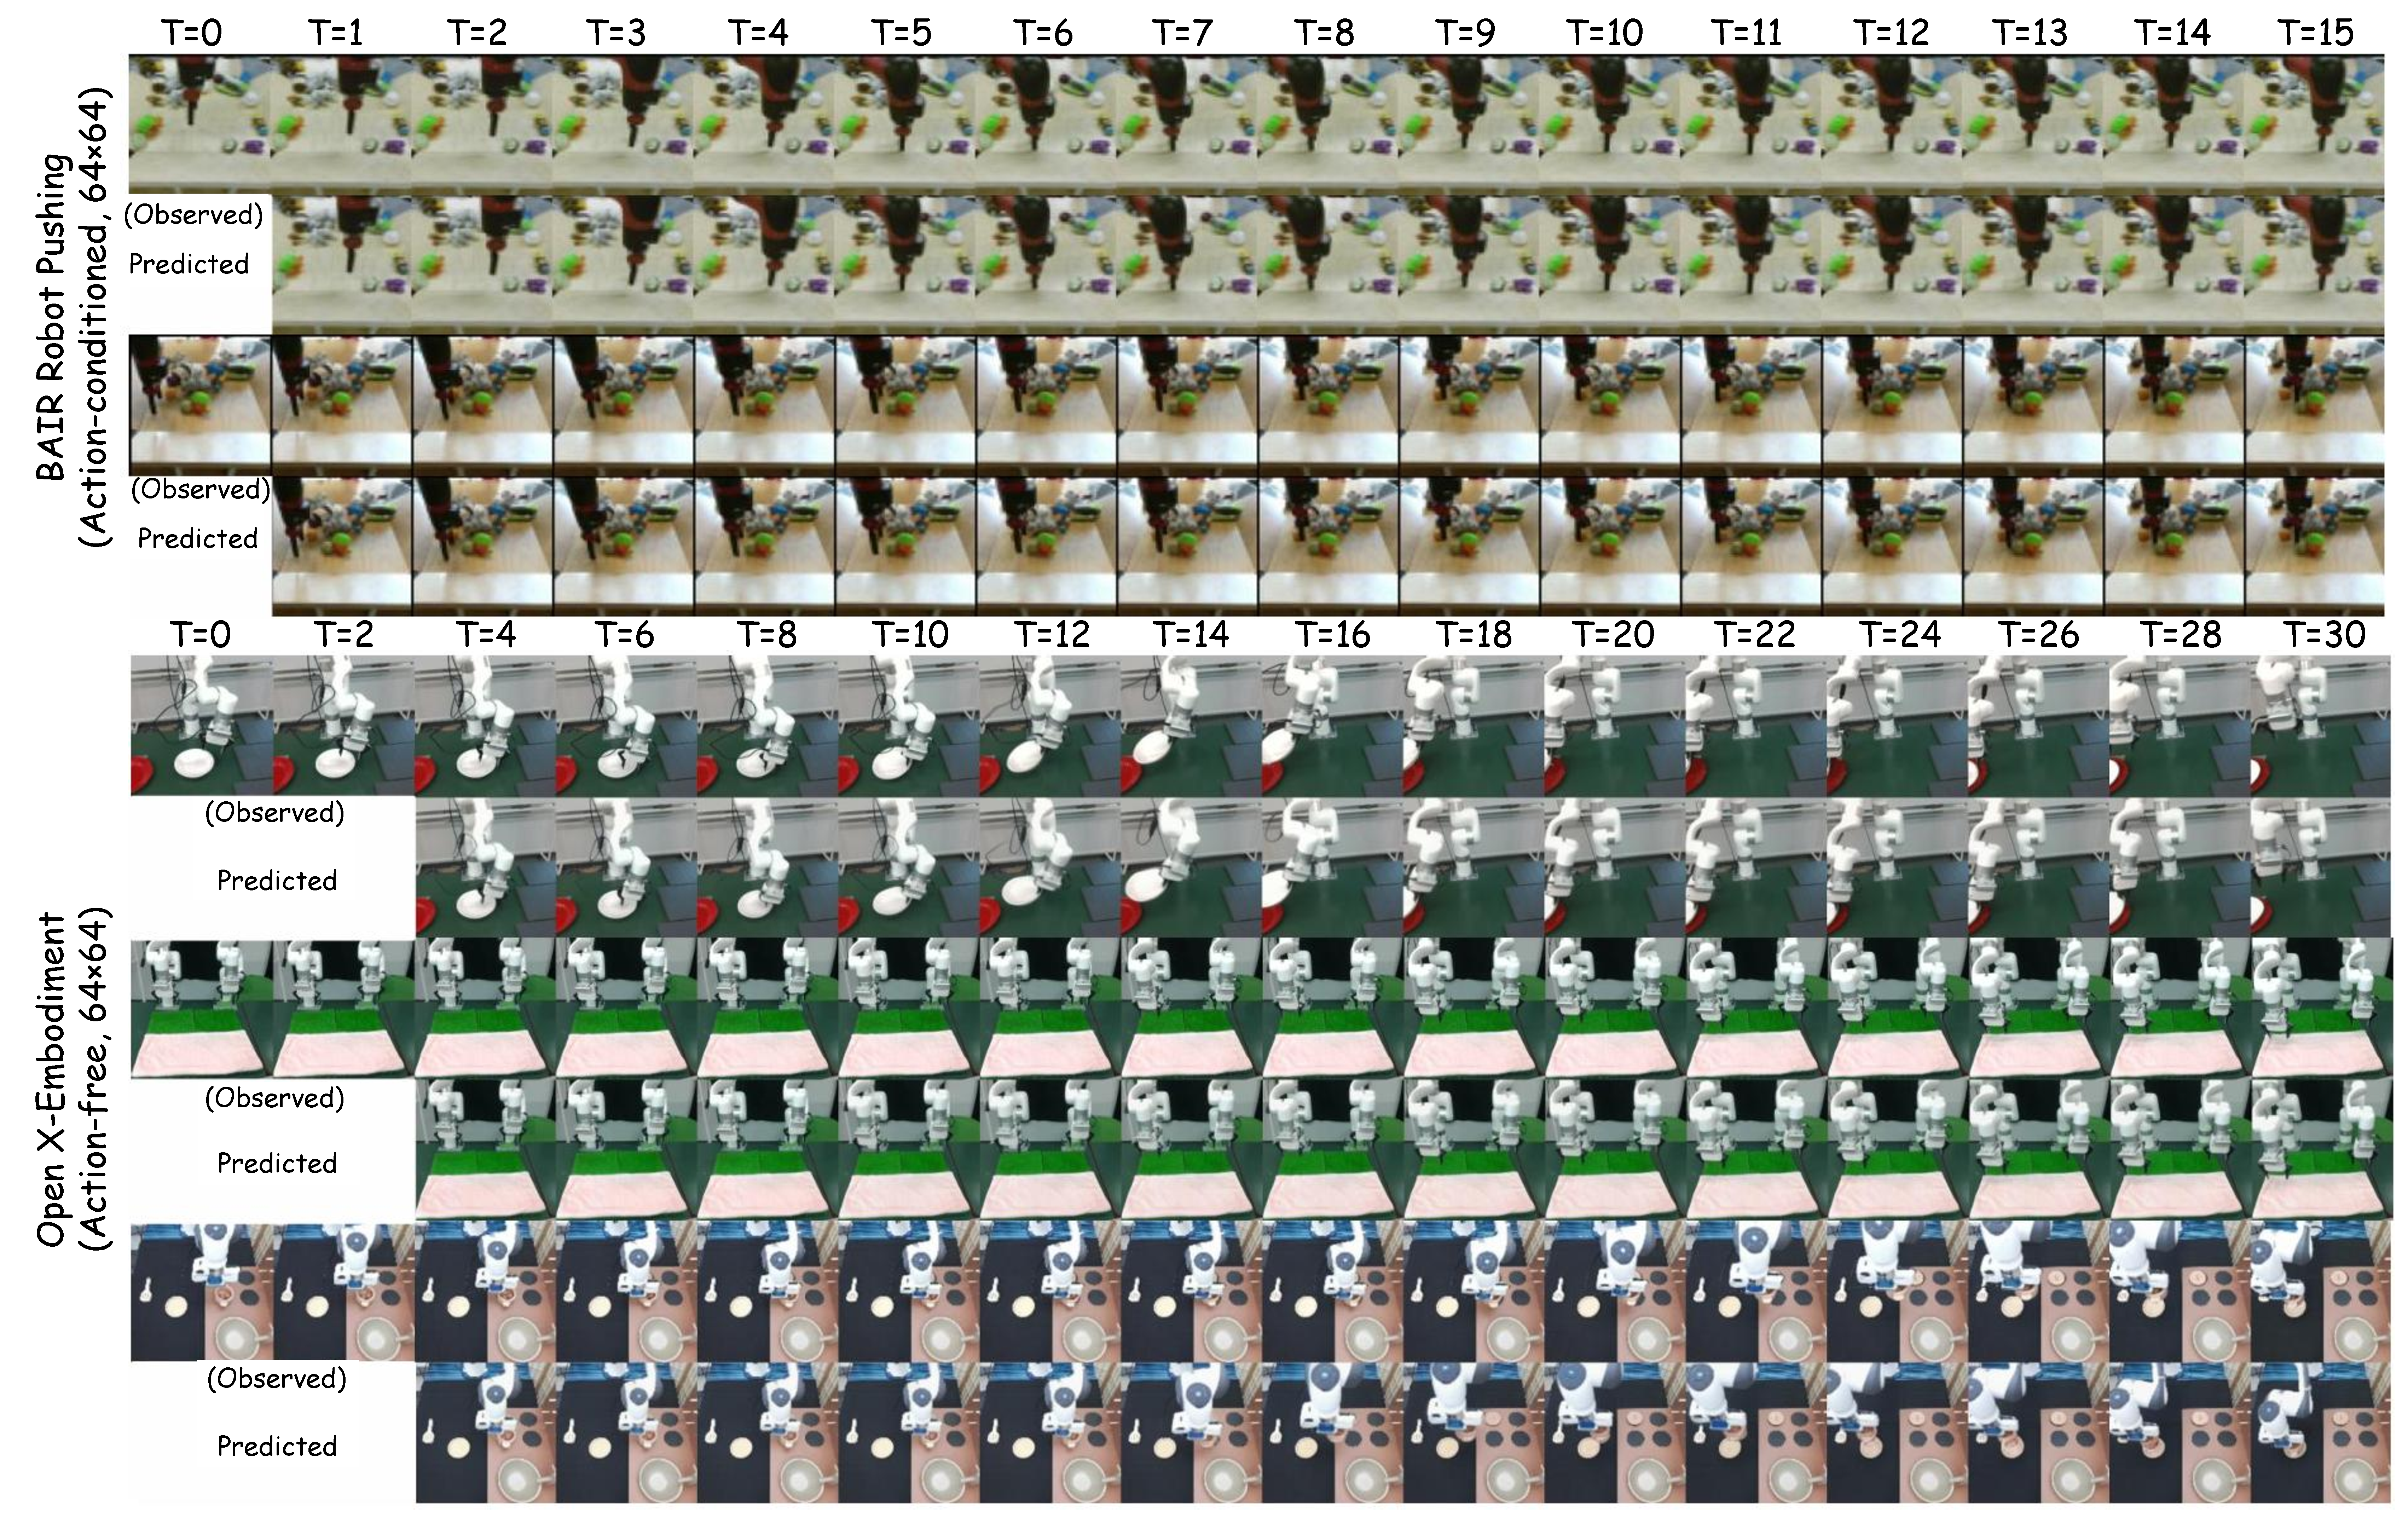
\includegraphics[width=1.0\linewidth]{fig_exp/fig64.pdf}
    \caption{\textbf{Visualization on BAIR and OpenX-Embodiment datasets.}}
    \label{fig_64}
    \vspace{-3ex}
\end{figure*}

\begin{figure*}[t]
    \centering
    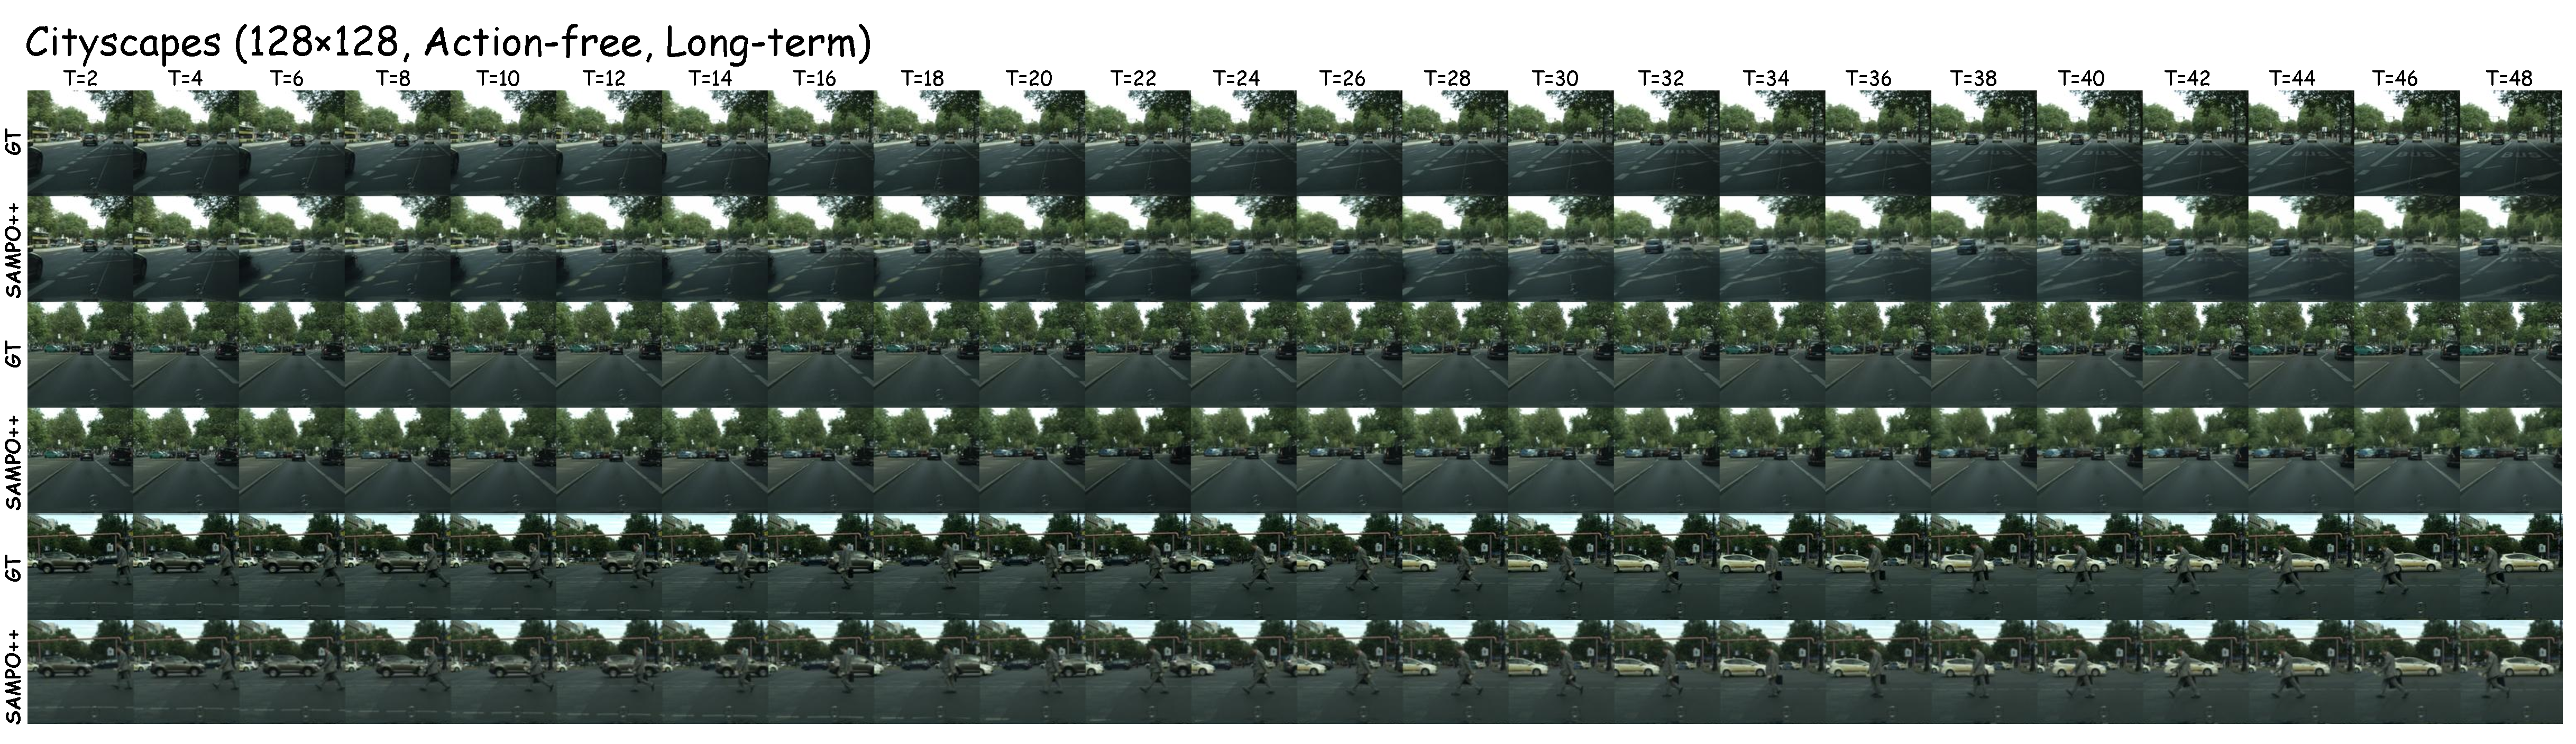
\includegraphics[width=1.0\linewidth]{fig_exp/fig_city.pdf}
    \caption{\textbf{Long-term video prediction on the Cityscapes dataset.} We visualize three distinct driving scenarios. Even over long-horizon generation, SAMPO++ excels at sustaining realistic scene dynamics and maintaining high spatiotemporal coherence without structural degradation. Zoom in for a better view.}
    \label{fig_city}
    \vspace{-3ex}
\end{figure*}

\begin{figure*}[t]
    \centering
    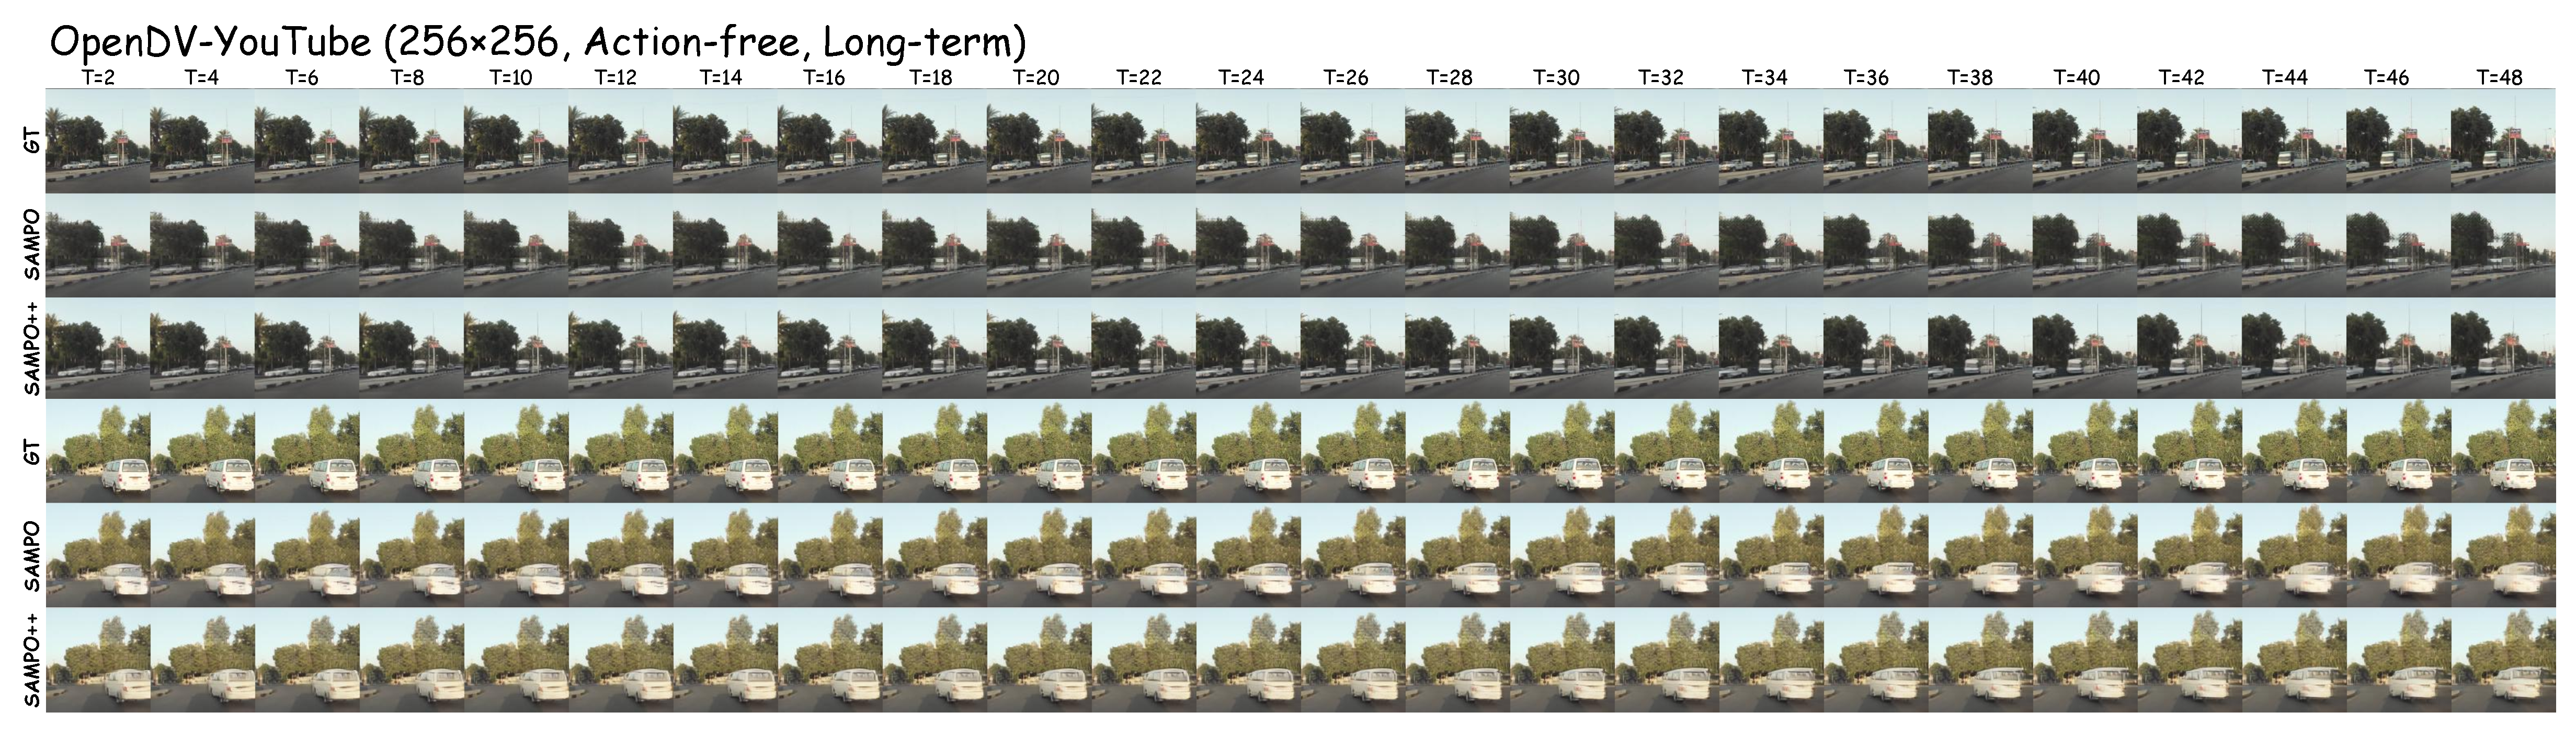
\includegraphics[width=1.0\linewidth]{fig_exp/figopendv.pdf}
    \caption{\textbf{High-resolution long-term video prediction on OpenDV-YouTube dataset.} We visualize highly complex, in-the-wild driving scenarios. While SAMPO suffers from severe temporal degradation in unconstrained driving scenarios, SAMPO++ effectively maintains robust dynamic modeling and strongly resists visual artifacts.}
    \label{fig_opendv}
    \vspace{-4ex}
\end{figure*}

\begin{figure}[t]
    \centering
    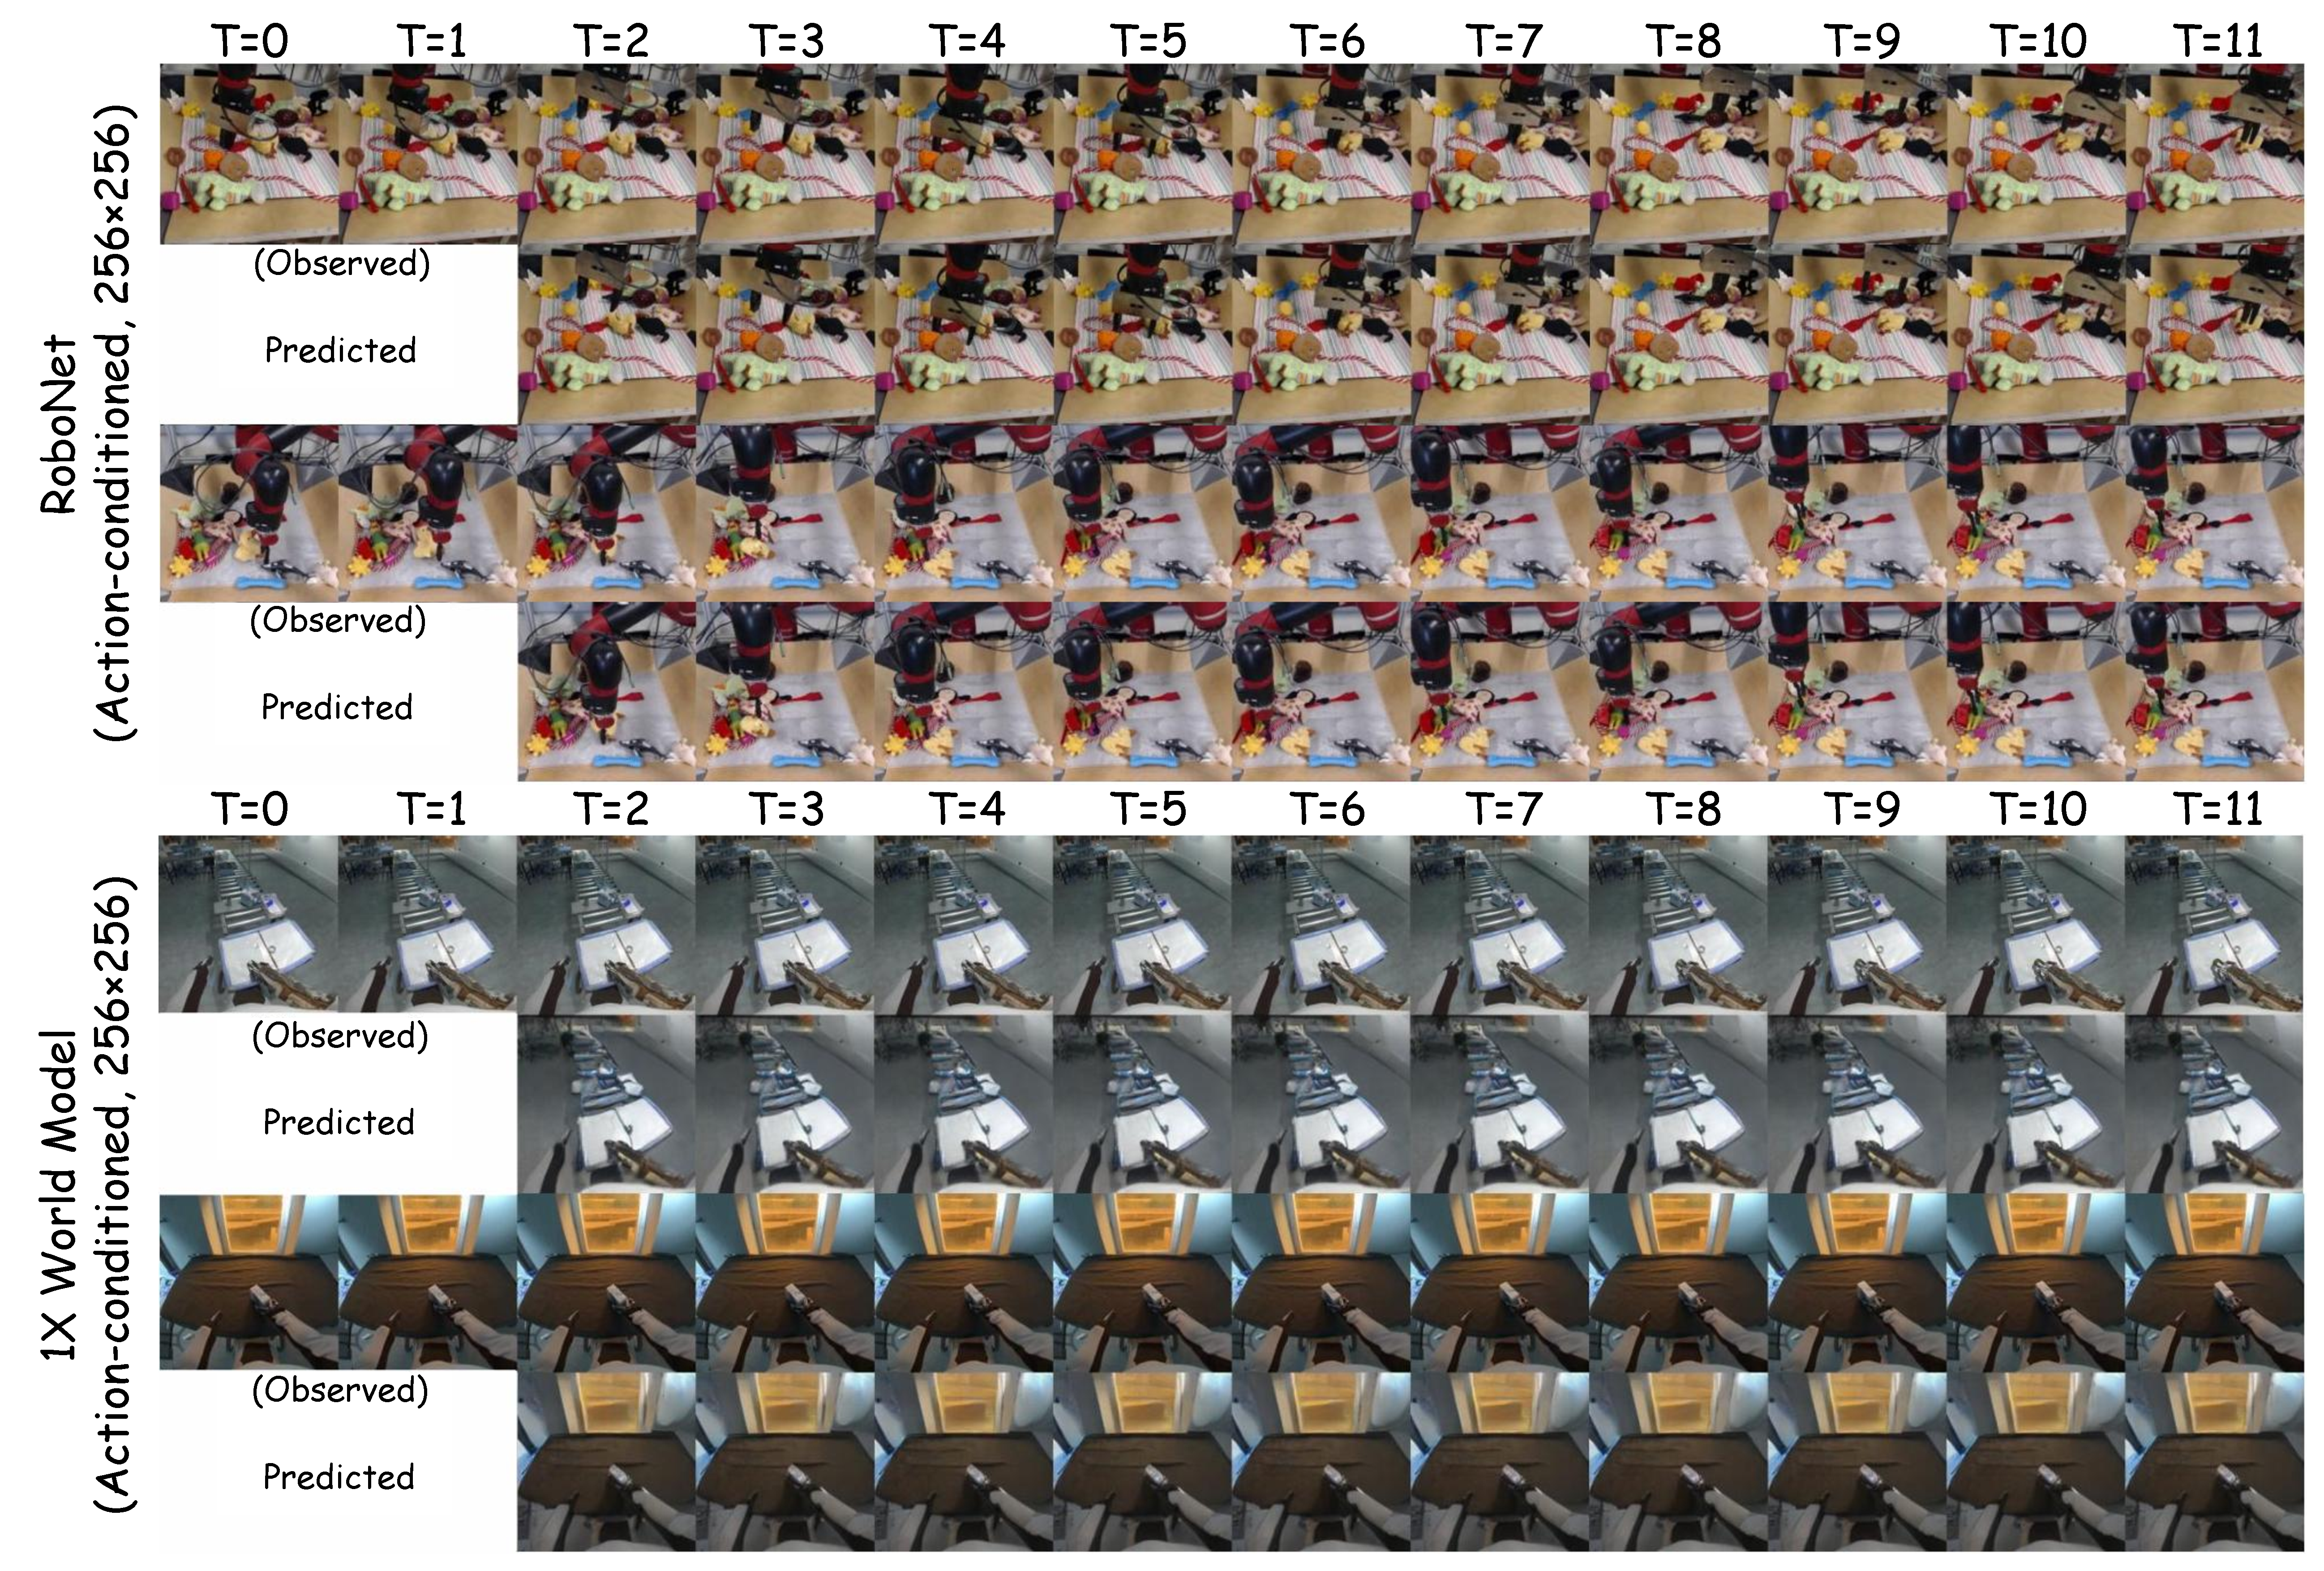
\includegraphics[width=1.0\linewidth]{fig_exp/fig256.pdf}
    \caption{\textbf{Visualization on RoboNet and 1X World Model.}}
    \label{fig_256}
    \vspace{-3ex}
\end{figure}

\begin{figure}[t]
    \centering
    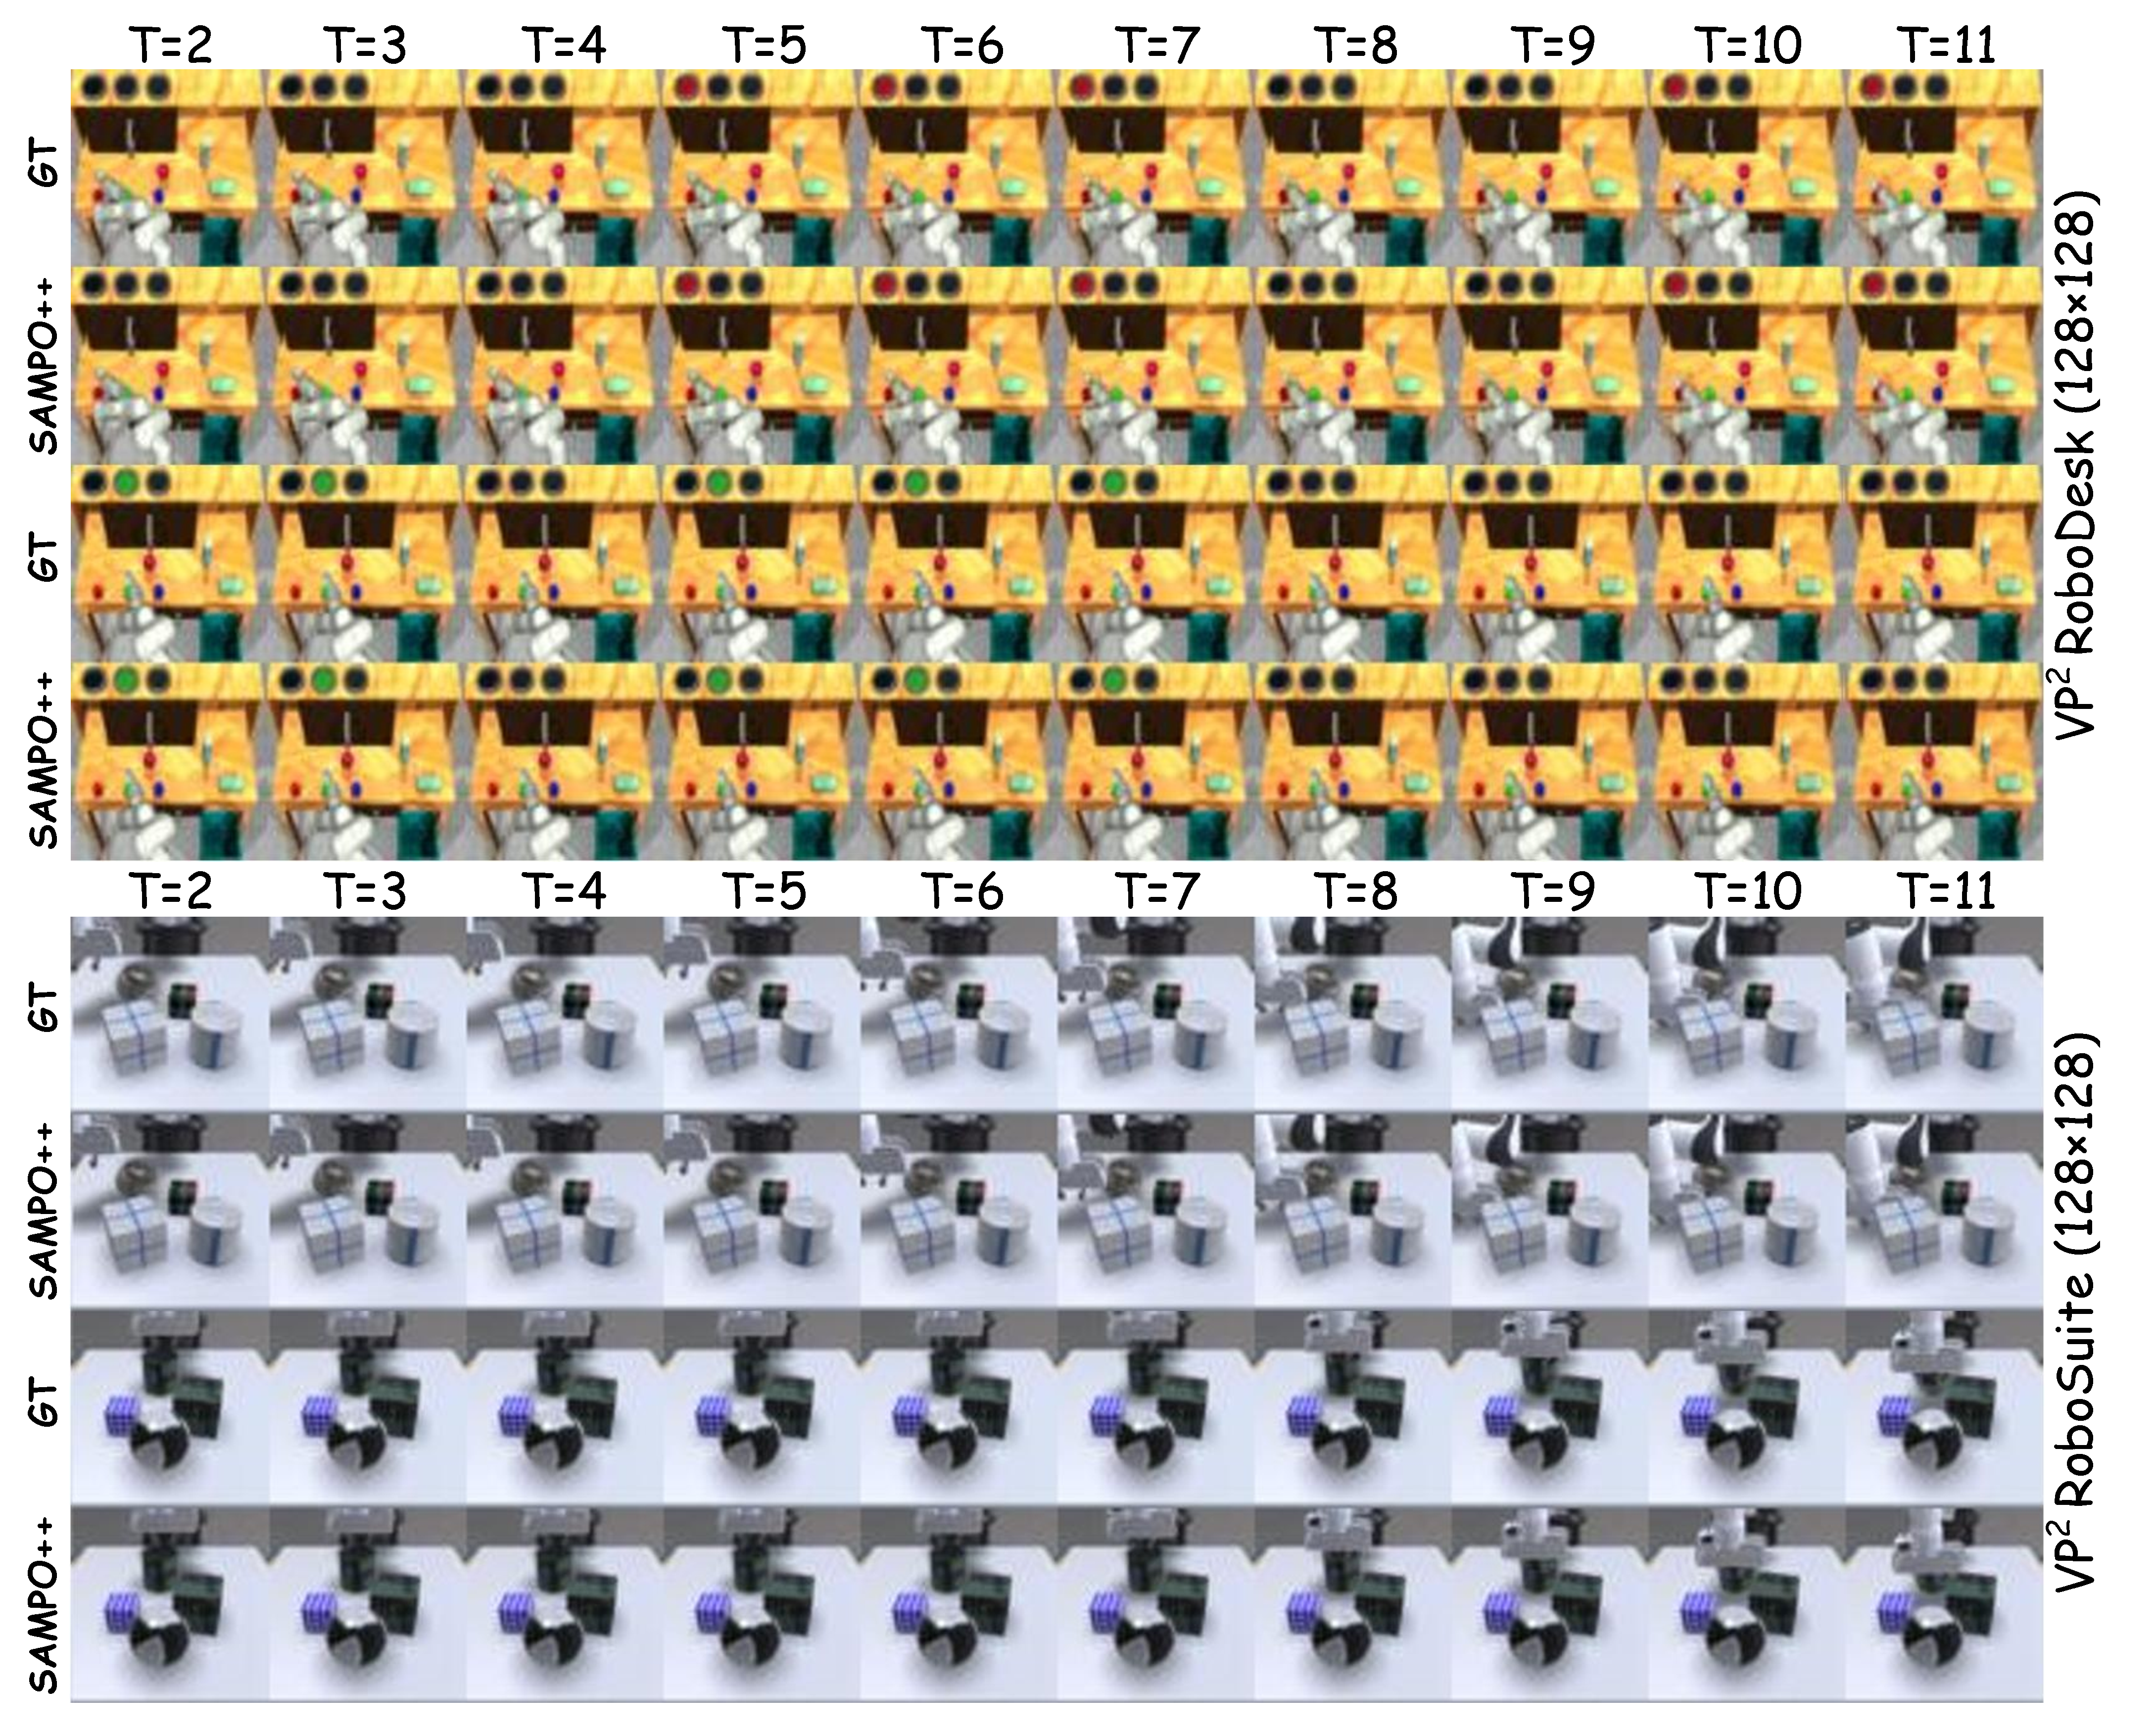
\includegraphics[width=1.0\linewidth]{fig_exp/fig_exp_vp2.pdf}
    \caption{\textbf{Visualization on the VP$^2$ benchmark.} We visualize two manipulation tasks from both the RoboDesk and RoboSuite environments.}
    % For each task, odd rows display the ground-truth observations, while even rows show the future trajectories predicted by SAMPO++.
    \label{fig_exp_vp2}
    \vspace{-3ex}
\end{figure}

\begin{figure}[t]
    \centering
    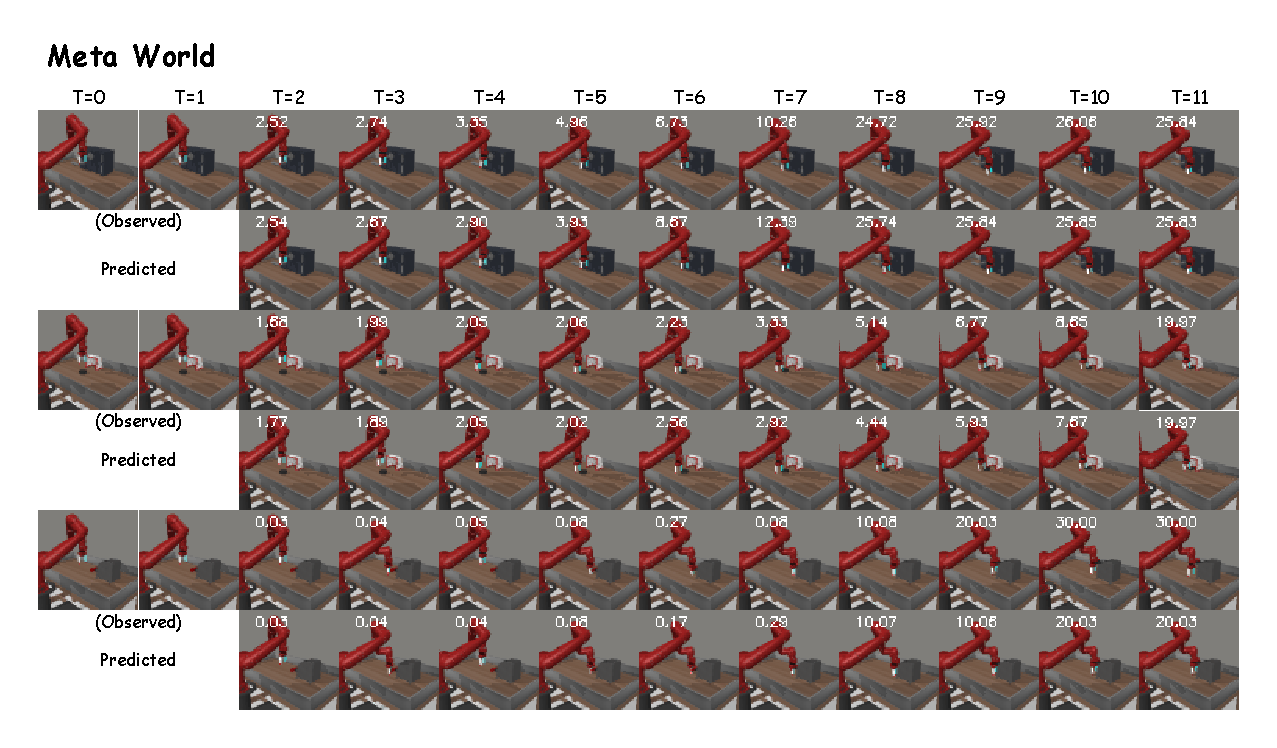
\includegraphics[width=1.0\linewidth]{fig_exp/fig_MW.pdf}
    \caption{\textbf{Visualization on the Meta-World tasks.} Each row corresponds to a different task: \textit{Coffee Push}, \textit{Door Lock}, \textit{Handle Pull Side}. Both actual reward and predicted reward are shown in the upper left corner.}
    \label{fig_MW}
    \vspace{-2ex}
\end{figure}

\subsection{Qualitative Analysis \& Visualization}

To contextualize our quantitative findings, we present a comprehensive qualitative analysis of SAMPO++ across diverse domains. Through a comparative visual assessment against ground-truth observations, we demonstrate the model's visual fidelity, physical plausibility, and strict adherence to action conditioning.

\textbf{Robotic Manipulation across Resolutions.} Figure~\ref{fig_64} showcases sampled rollouts on the BAIR and Open X-Embodiment datasets, illustrating the model's capacity to maintain spatiotemporal coherence across highly diverse manipulation trajectories at standard resolutions. Extending this to high-resolution generation, Figure~\ref{fig_256} presents $256 \times 256$ rollouts on the RoboNet and 1X World Model datasets. Here, SAMPO++ accurately synthesizes fine-grained physical details—such as subtle humanoid articulations—while preserving object permanence over extended horizons.

\textbf{Action-Conditioned Rollouts for Control.} Moving beyond passive video prediction, we examine interactive rollouts conditioned on specific action sequences. Figure~\ref{fig_exp_vp2} illustrates representative tasks from the $\text{VP}^2$ benchmark. By contrasting the predicted trajectories with ground-truth observations, we verify that the generated dynamics strictly obey the injected control signals and accurately simulate continuous physical interactions. Furthermore, Figure~\ref{fig_MW} demonstrates long-term rollouts on Meta-World manipulation tasks. The model reliably predicts both the visual observations and the corresponding task rewards at each step, yielding a robust neural simulator for downstream planning and policy learning.

\textbf{In-the-Wild and Autonomous Driving Generalization.} Finally, we demonstrate the scalability of our continuous-flow framework to complex, unconstrained environments. Figure~\ref{fig_city} displays long-term video prediction on the Cityscapes dataset, where SAMPO++ successfully renders dynamic traffic scenarios and preserves background structural integrity despite rapid viewpoint transformations. To further push these boundaries, Figure~\ref{fig_opendv} visualizes high-resolution ($256 \times 256$) long-horizon rollouts on uncurated internet videos from the OpenDV-YouTube dataset. Even when confronted with massive pixel displacements and unpredictable ego-motion, the model maintains robust spatiotemporal coherence, confirming its strong generalization capabilities in real-world driving scenarios.

\section{Conclusion and Discussion}
\label{Sec5:Conclusion}

In this work, we presented SAMPO++, a unified continuous-flow world modeling framework that reconciles high-resolution scalability, interactive efficiency, and long-horizon spatiotemporal coherence. 
By explicitly decoupling inter-frame causal dynamics from intra-frame detail refinement, we synergize an asymmetric continuous tokenizer, hierarchical flow matching, and Action-adaptive Dynamics Modulation (ADM) for precise physical control.
To overcome error accumulation in continuous state spaces, we proposed a Scale-Aware spacetime RoPE (SA-RoPE) and a rollout-aware consistency learning strategy. By utilizing cross-frame latent correction, this mechanism aligns the training objective with autoregressive inference, effectively mitigating unbounded latent drift. 
Extensive evaluations demonstrate that SAMPO++ achieves unprecedented long-term rollout fidelity, establishing it as a robust neural simulator for visual planning and reinforcement learning.
Ultimately, expanding this continuous latent manifold for cross-embodiment generalization represents a promising frontier for foundational embodied intelligence.



\newpage



% \begin{abstract}

Action-conditioned world models are fundamental for embodied agents to simulate future environments and execute long-horizon planning. Yet, current methodologies struggle with a persistent dichotomy: discrete autoregressive models offer robust causal reasoning but suffer from quantization artifacts and resolution bottlenecks, while continuous generative models yield high perceptual fidelity but lack the structured temporal consistency necessary for reliable planning. 
To bridge this divide, we propose SAMPO++, a unified framework that seamlessly integrates temporal autoregressive modeling with scale-wise flow matching within a fully continuous latent space. 
\textcolor{blue}{At its core, SAMPO++ introduces a novel ``Predict-then-Refine" paradigm: a temporal autoregressive transformer first establishes coarse-grained structural priors for future states, which a scale-wise flow matching generator subsequently refines to synthesize high-fidelity details from noise. 
To achieve precise controllability, we design an Action-adaptive Dynamics Modulation (ADM) mechanism that injects action signals into feature statistics via scale-aware affine transformations. 
Moreover, we mitigate long-term structural degradation by incorporating Scale-Aware spacetime Rotary Position Embeddings (SA-RoPE) alongside a flow trajectory rectification strategy, thereby enforcing rigorous spatiotemporal coherence. }
Extensive empirical evaluations demonstrate that SAMPO++ significantly surpasses state-of-the-art discrete and continuous baselines in video prediction quality, dynamic consistency, and control responsiveness, setting a new benchmark for high-fidelity continuous world modeling.

\end{abstract}

\begin{IEEEkeywords}
Generalizable Robot Manipulation, Average Velocity Field, Region-Aware Perception.
\end{IEEEkeywords}
% \input{sec/Blue1intro}
% \input{sec/Blue2related}
% \input{sec/Blue3method}
% \input{sec/Blue4experiment}
% \input{sec/Blue5conclusion}

\ifCLASSOPTIONcaptionsoff
  \newpage
\fi

\bibliography{egbib}
\bibliographystyle{IEEEtran}

\begin{IEEEbiography}[{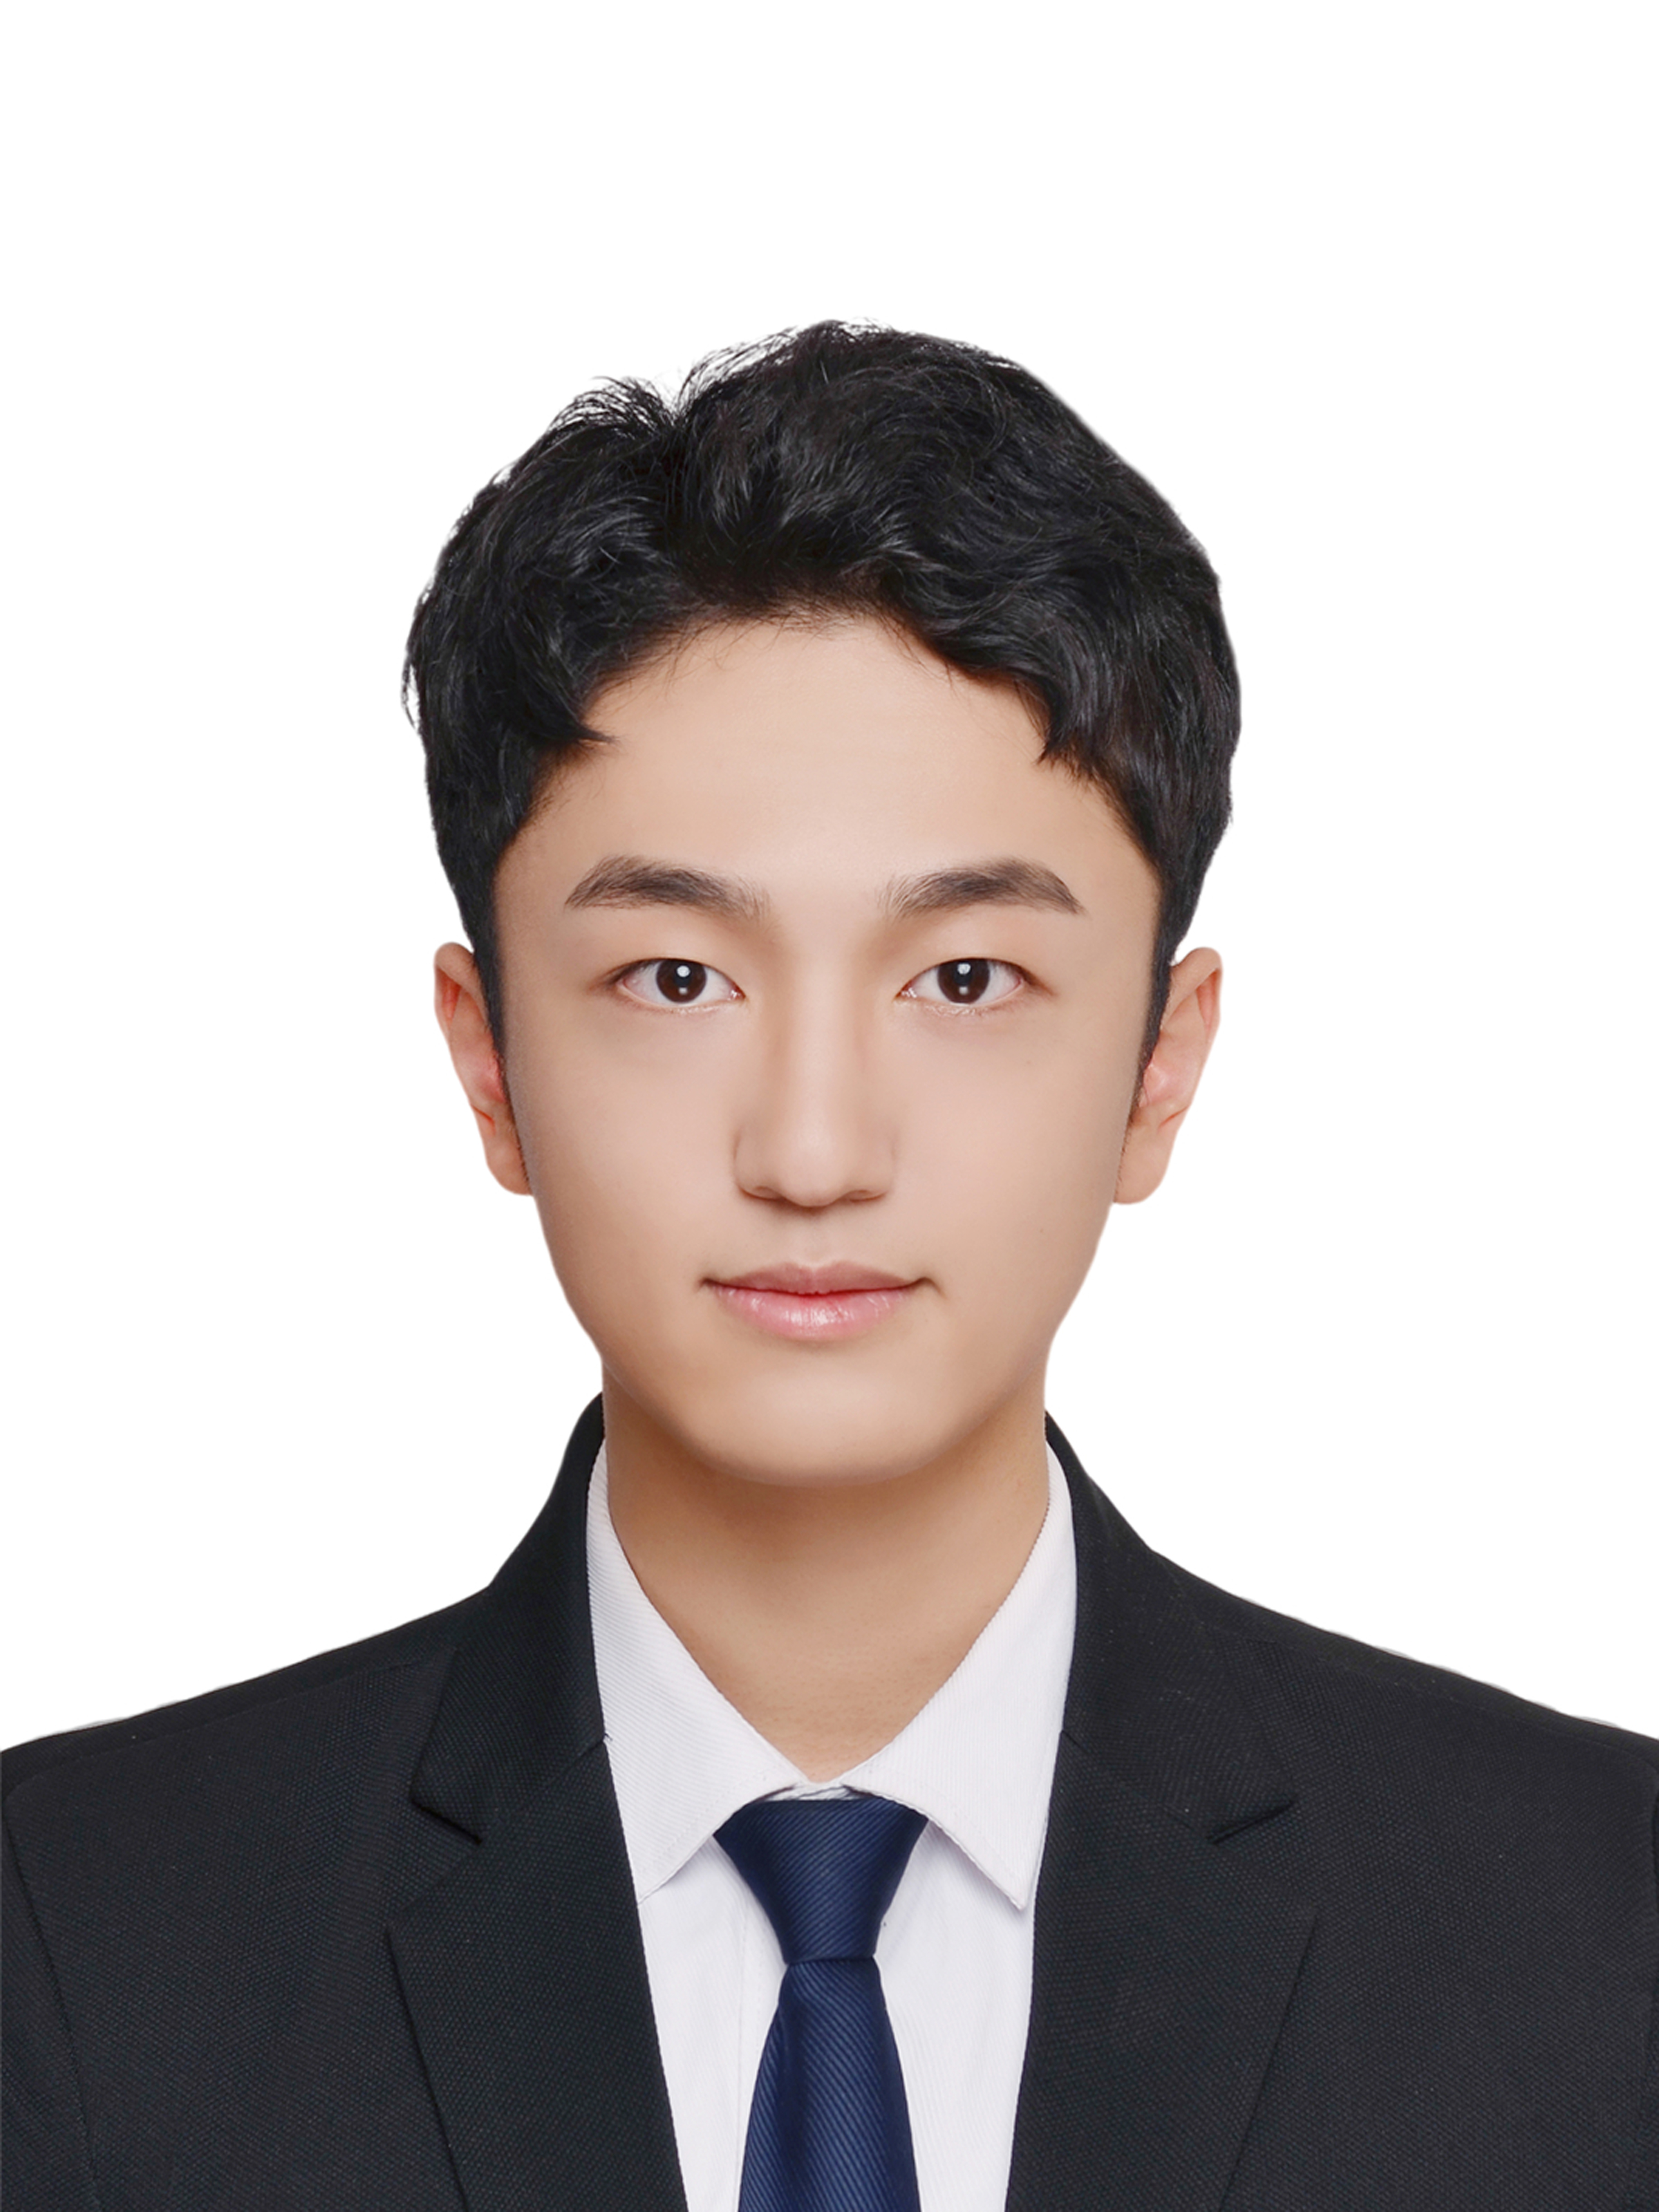
\includegraphics[width=1in,height=1.25in,clip,keepaspectratio]{fig/author/senwang.jpg}}]{Sen Wang} received the B.E. degree in Control Science and Engineering from Jilin University, Changchun, China, in 2023.
He is currently a third-year Ph.D. candidate in the Institute of Artificial Intelligence and Robotics at Xi’an Jiaotong University. His research interests include embodied computer vision, robotic manipulation and interactive world model. 
% He has published four papers in CVPR and NIPS.
\end{IEEEbiography}


\begin{IEEEbiography}[{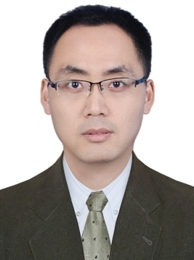
\includegraphics[width=1in,height=1.25in,clip,keepaspectratio]{fig/author/sanpingzhou.png}}]{Sanping Zhou} (Member, IEEE) received the Ph.D.
 degree in control science and engineering from Xi'an Jiaotong University, Xi’an, China, in 2020. From 2018 to 2019, he was a visiting Ph.D. student with
 Robotics Institute, Carnegie Mellon University. He is currently a professor with the Institute of Artificial Intelligence and Robotics, Xi'an Jiaotong University.
 His research interests include machine learning, deep learning, computer vision, and embodied AI, with a focus on person re-identification, salient object detection, medical image segmentation, image classification, and visual tracking.
\end{IEEEbiography}



% \begin{IEEEbiography}[{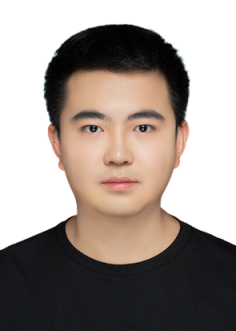
\includegraphics[width=1in,height=1.25in,clip,keepaspectratio]{fig/author/hch.png}}]{Hongcheng Huo} is an undergraduate student in Computer Science and Mathematics at the University of Toronto. His research experience includes work on multi-armed bandit algorithms in reinforcement learning, numerical analysis with a focus on high-performance computing and numerical optimization, and data-driven modeling using machine learning and deep learning. His academic interests focus on machine learning, deep learning, and efficient algorithmic modeling.
% \end{IEEEbiography}

\begin{IEEEbiography}[{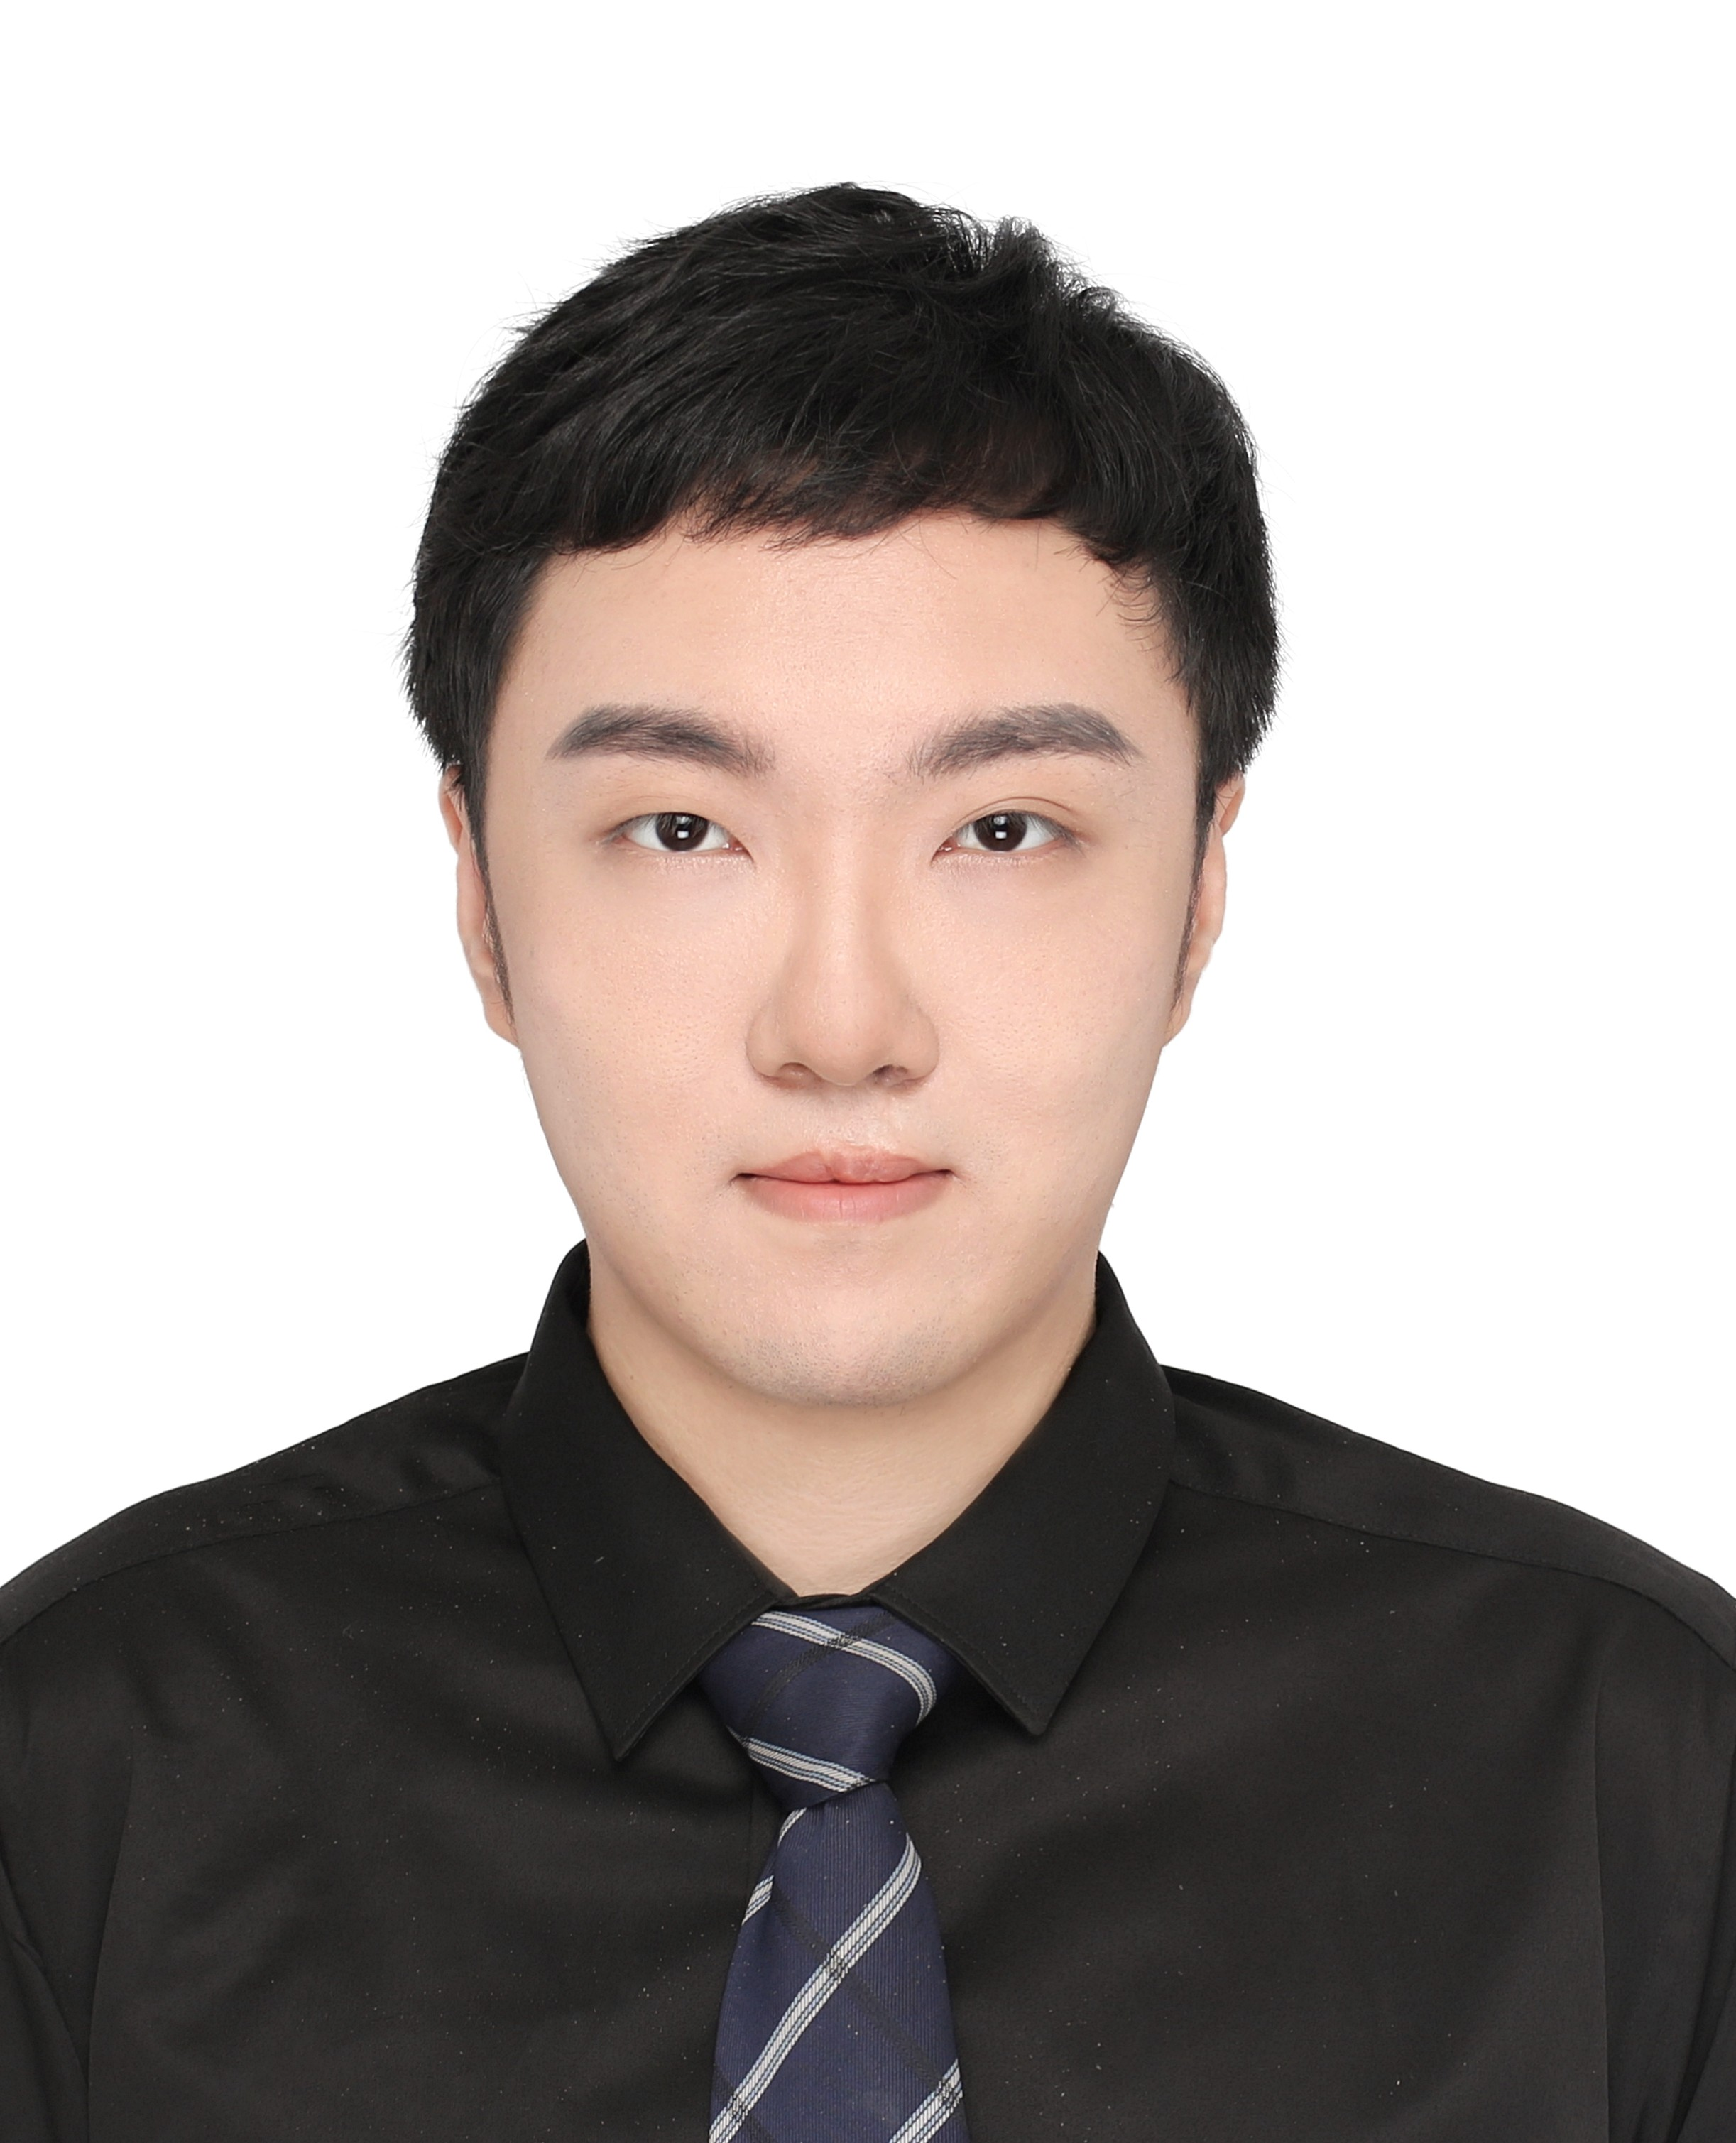
\includegraphics[width=1in,height=1.25in,clip,keepaspectratio]{fig/author/dhy.jpg}}]{Huaiyi Dong} received the B.E. degree in Software Engineering from China University of Geosciences,  wuhan, China, in 2023. He is currently a Ph.D. candidate in the Institute of Artificial Intelligence and Robotics at Xi’an Jiaotong University. His research interests include embodied computer vision and robotic manipulation. 
% He has published four papers in CVPR and NIPS.
\end{IEEEbiography}
\vspace{-6ex}

\begin{IEEEbiography}[{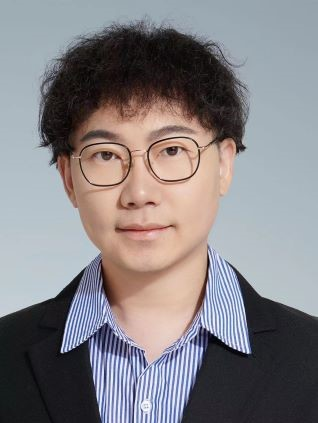
\includegraphics[width=1in,height=1.25in,clip,keepaspectratio]{fig/author/Kun-Xia.jpg}}]{Kun Xia} received the Ph.D. degree in Control Science and Engineering from Xi'an Jiaotong University, Xi'an, China, in 2024. From 2022 to 2023, he was a visiting Ph.D. student with University of Illinois Chicago, IL, USA. He is currently an Assistant Professor with the School of Computer Science and Technology, Xi'an Jiaotong University, Xi'an, China. His research interests include computer vision, image/video processing, analysis and understanding.
\end{IEEEbiography}
\vspace{-6ex}

\begin{IEEEbiography}[{\includegraphics[width=1in,height=1.25in,clip,keepaspectratio]{fig/author/Gang-Hua1.pdf}}]{Gang Hua}
(Fellow, IEEE) received the B.S. and M.S. degrees in automatic control engineering from Xi’an Jiaotong University, Xi’an, China, in 1999 and 2002, respectively, and the Ph.D. degree in electrical engineering and computer science from Northwestern University, Evanston, IL, USA, in 2006. He was a senior scientist with Microsoft Live labs Research from 2006 to 2009, a senior researcher with Nokia Research Center Hollywood from 2009 to 2010, a research staff member with IBM Research T. J. Watson Center from 2010 to 2011, and a visiting researcher from 2011 to 2014. During 2014–15, he took a leave and worked on the Amazon-Go project. He was an associate professor with the Stevens Institute of Technology from 2011 to 2015. He was also with Microsoft from 2015 to 2018 as the Science/Technical adviser to the CVP of the Computer Vision Group, director of Computer Vision Science Team in Redmond, Taipei ATL, and senior principal researcher/research manager with Microsoft Research. He was the CTO with Convenience Bee, and the managing director and chief scientist of its research branch in US, Wormpex AI Research, from 2018 to 2024. He was the vice president with Multimodal Experiences Research Lab, Dolby Laboratories from 2024 to 2025. He is currently the director of applied science with Amazon Alexa AI. His research interests include computer vision, pattern recognition, machine learning, robotics, towards general artificial intelligence, with primary applications in cloud and edge intelligence. He is an associate editor for TPAMI and MVA. He is a general chair of ICCV’2027 and a program chair of CVPR’2019 \& 2022. He is the recipient of the 2015 IAPR Young Biometrics Investigator Award. He is an IAPR Fellow and an ACM distinguished scientist.
\end{IEEEbiography}
\vspace{-6ex}

\begin{IEEEbiography}[{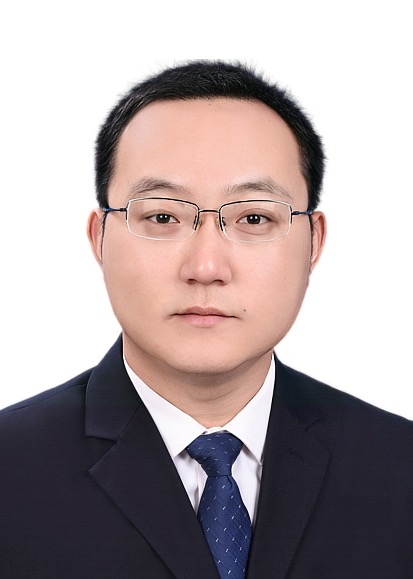
\includegraphics[width=1in,height=1.25in,clip,keepaspectratio]{fig/author/lewang.jpg}}]{Le Wang}(Senior Member, IEEE) received the B.S. and Ph.D. degrees in control science and engineering from Xi’an Jiaotong University, Xi’an, China, in 2008 and 2014, respectively. From 2013 to 2014, he was a visiting Ph.D. student with the Stevens Institute of Technology, Hoboken, NJ, USA. From 2016 to 2017, he was a visiting scholar with Northwestern University, Evanston, IL, USA. He is currently a professor with the Institute of Artificial Intelligence and Robotics, Xi’an Jiaotong University. His research interests include computer vision, pattern recognition, machine learning, and robotic manipulation. He is an associate editor for PR, MVA, and PRL.
\end{IEEEbiography}




\end{document}
